%\documentclass[11pt]{scrbook} % use larger type; default would be 10pt

% WITH BLEED
% US Trade => 6x9, with a 0.125 bleed
% Adjust images size and gutter so tabs bleed by .125
% See https://www.createspace.com/Products/Book/InteriorPDF.jsp
\documentclass[paper=6.14in:9.21in,pagesize=pdftex,11pt,twoside,openright]{scrbook}
%openright
% Paper width
% W = 6.125in (6+0.125 --- bleed)
% Paper height
% H = 9.25in (9+2*.125 --- bleed)
% Paper gutter
% BCOR = 0.375in (0.5+0.5-0.625 --- margin with bleed)
% Margin (0.5in imposed on lulu, recommended on createspace)
% m = 0.625in (0.5+0.125 --- bleed)
% Text height
% h = H - 2m = 8in
% Text width
% w = W - 2m - BCOR = 4.5in
\areaset[0.375in]{4.5in}{8in}
\usepackage[utf8]{inputenc} % set input encoding (not needed with XeLaTeX)

%%% Examples of Article customizations
% These packages are optional, depending whether you want the features they provide.
% See the LaTeX Companion or other references for full information.

%\usepackage{mitpress}
\usepackage{framed}

\usepackage[top=1in, bottom=1in, left=1in, right=1in]{geometry}

\usepackage{graphicx} % support the \includegraphics command and options
%\usepackage{wrapfig}

% \usepackage[parfill]{parskip} % Activate to begin paragraphs with an empty line rather than an indent

%%% PACKAGES
\usepackage{booktabs} % for much better looking tables
\usepackage{array} % for better arrays (eg matrices) in maths
\usepackage{paralist} % very flexible & customisable lists (eg. enumerate/itemize, etc.)
\usepackage{verbatim} % adds environment for commenting out blocks of text & for better verbatim
\usepackage{subfig} % make it possible to include more than one captioned figure/table in a single float
% These packages are all incorporated in the memoir class to one degree or another...
\usepackage{makeidx}
\usepackage{amsmath}
\usepackage{amsfonts}
\usepackage[font={small,it}]{caption}
\usepackage{url}
\usepackage{hyperref}
\usepackage{harvard}
\usepackage{marginnote}

%%% HEADERS & FOOTERS
%\usepackage{fancyhdr} % This should be set AFTER setting up the page geometry
%\pagestyle{fancy} % options: empty , plain , fancy
%\renewcommand{\headrulewidth}{0pt} % customise the layout...
%\lhead{}\chead{}\rhead{}
%\lfoot{}\cfoot{\thepage}\rfoot{}

%%% SECTION TITLE APPEARANCE
\usepackage{sectsty}
\allsectionsfont{\sffamily\mdseries\upshape} % (See the fntguide.pdf for font help)
% (This matches ConTeXt defaults)

%%% ToC (table of contents) APPEARANCE
\usepackage[nottoc,notlof,notlot]{tocbibind} % Put the bibliography in the ToC
\usepackage[titles,subfigure]{tocloft} % Alter the style of the Table of Contents
\renewcommand{\cftsecfont}{\rmfamily\mdseries\upshape}
\renewcommand{\cftsecpagefont}{\rmfamily\mdseries\upshape} % No bold!

\newcommand{\screencast}[2]{
  \marginnote{\href{#1}{\includegraphics[width=1.5cm]{figs/youtube/#2}}}}


%%% END Article customizations

%%% The ``real'' document content comes below...
\makeindex

%\title{Introduction to Autonomous Robots}
%\author{Nikolaus Correll}
%\date{} % Activate to display a given date or no date (if empty),
         % otherwise the current date is printed 

\begin{document}
%\maketitle

\thispagestyle{empty}
\begin{flushleft}
Nikolaus Correll\\
Introduction to Autonomous Robots, 1st edition, \today\\
ISBN-13: 978-1493773077
\end{flushleft}

\vfill

\begin{figure}[!h]

\includegraphics[width=1in]{figs/by-nc-nd}
\end{figure}

This book is licensed under a Creative Commons Attribution-NonCommercial-NoDerivs 3.0 Unported License. You are free to share, i.e., copy, distribute and transmit the work under the following conditions: You must attribute the work to its main author, you may not use this work for commercial purposes, and you may not alter, transform, or create derivatives of this work, except for written permission by the author. For more information, please consult \url{http://creativecommons.org/licenses/by-nc-nd/3.0/deed.en_US}.


\cleardoublepage
\thispagestyle{empty}
\topskip0pt
\vspace*{\fill}
\begin{center}
For Arthur, Tatiana, Benedict and Silvester\\
future robot users
\end{center}
\vspace*{\fill}

\tableofcontents

\chapter*{Preface}
This book provides an algorithmic perspective to autonomous robotics to students with a sophomore-level of linear algebra and probability theory. Robotics is an emerging field at the intersection of mechanical and electrical engineering with computer science. With computers becoming more powerful, making robots smart is getting more and more into the focus of attention and robotics research most challenging frontier. While there are a large number of textbooks on the mechanics and dynamics of robots that address sophomore-level undergraduates available, books that provide a broad algorithmic perspective are mostly limited to the graduate level. This book has therefore been developed not to create ``yet another textbook, but better than the others'', but to allow me to teach robotics to the 3rd and 4th year undergraduates at the Department of Computer Science at the University of Colorado. 

Although falling under the umbrella of ``Artificial Intelligence'', standard AI techniques are not sufficient to tackle problems that involve uncertainty, such as a robot's interaction in the real world. This book uses simple trigonometry to develop the kinematic equations of simple manipulators and mobile robots, then introduces path planning, sensing, and hence uncertainty. The robot localization problem is introduced by formally introducing error propagation, which leads to Markov localization, the Particle filter and finally the Extended Kalman Filter, and Simultaneous Localization and Mapping. 

Instead of focusing on the state-of-the-art solutions to a particular sub-problem, emphasis of the book is on a concise step-by-step development and recurrent examples that capture the essence of a problem, but might not necessarily be the best solution. For example, odometry and line-fitting are used to explain forward kinematics and least-squares solutions, respectively, and later serve as motivating examples for error propagation and the Kalman filter in a localization context.

Also, the book is explicitely robot-agnostic, reflecting the timeliness of fundamental concepts. Instead, a series of possible project-based curricula are described in an Appendix and available online, ranging from a maze-solving competition that can be realized with most miniature differential-wheel robots that include a camera to manipulation experiments with the Baxter robot, all of which can be entirely conducted in simulation. 

This book is released under a Creative Commons license, which allows anyone to copy and share this book, although not for commercial purposes and not to create derivatives of these works. This license comes very close to the ``copyright'' of a standard textbook, except that you are free to copy it for non-commercial purposes. I have chosen this format as it seems to maintain the best trade-off between a freely available textbook resource that others hopefully contribute to and maintaining a consistent curriculum that others can refer to. 

Writing this book would not have been possible without the excellent work of others before me, most notably ``Introduction to Robotics: Mechanics and Control'' by John Craig and ``Introduction to Autonomous Mobile Robots'' by Roland Siegwart, Illah Nourbakhsh and David Scaramuzza, and innumerable other books and websites from which I learned and borrowed examples and notation.

\begin{flushright}
Nikolaus Correll\\
Boulder, Colorado, \today
\end{flushright}

\chapter{Introduction}\label{chap:introduction}
Robotics celebrated its 50th birthday in 2011, dating back to the first commercial robot in 1961 (the Unimate). In a ``Tonight Show'' from the time, this robot did amazing things: it opens a bottle of beer, pours it, puts a golf ball into the hole, and even conducts an orchestra. This robot does all what we expect a good robot to do: it is dexterous, it is accurate, and even creative. Since this robot's appearance on the Tonight show, more than 50 years have passed --- so how incredible must be the capabilities of today's robots and what must they be able to do?

Interestingly, we just recently learned doing all the things demonstrated by Unimate autonomously. Unimate indeed did what was shown on TV, but all motions have been preprogrammed and the environment has been carefully staged.  Only the advent of cheap and powerful sensors and computation has recently enabled robots to detect an object by themselves, plan motions to it and grasp it. Yet, robotics is still far away from doing these tasks with human-like performance.

This book introduces you to the computational fundamentals of autonomous robots. Robots are \emph{autonomous} when they make decisions in response to their environment vs.\ simply following a pre-programmed set of motions. They achieve this using techniques from signal processing, control theory, and artificial intelligence, among others. These techniques are coupled with the mechanics, the sensors, and the actuators of the robot. Designing a robot therefore requires a deep understanding of both algorithms and its interfaces to the physical world.

The goals of this introductory chapter are to introduce the kind of problems roboticists deal with and how they solve it.

\section{Intelligence and embodiment}
Our notion of ``intelligent behavior'' is strongly biased by our understanding of the brain and how computers work: intelligence is located in our heads. In fact, however, a lot of behavior that looks intelligent can be achieved by very simple means. For example, mechanical wind-up toys can avoid falling of an edge simply by using a fly-wheel that rotates at a right angle to their direction of motion and a caster wheel. Once the caster wheel looses contact with the ground---that is the robot has reached the edge---the fly-wheel kicks in and pulls the robot to the right (Figure \ref{fig:winduptoy}). 

\begin{figure}
	\centering
		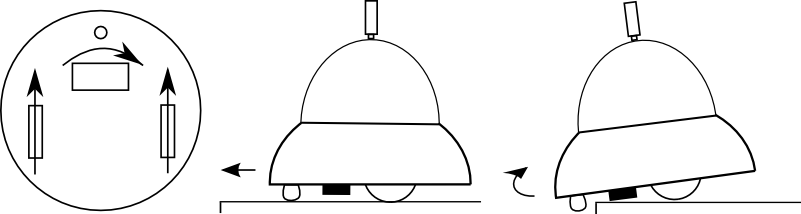
\includegraphics[width=\textwidth]{figs/winduptoysketch.png}
	\caption{A wind-up toy that does not fall of the table using purely mechanical control. A fly-wheel that turns orthogonal to the robot's motion induces a right turn as soon as it hits the ground once the front caster wheel goes off the edge.}
	\label{fig:winduptoy}
\end{figure}

A robot vacuum cleaner might solves the same problem very differently: it employs infrared sensors that are pointed downwards to detect edges such as stairs and then issues a command to make an avoiding turn. Once electronics are on-board, this is a much more efficient, albeit much more complex, approach.

Whereas the above examples provide different approaches to implement intelligent behaviors, similar trade-offs exist for robotic planning. For example, ants can find the shortest path between their nest and a food source by simply choosing the trail that already has more pheromones, the chemicals ants communicate with, on it. As shorter paths will have ants not only go faster to the food, but also return faster, its pheromone trail builds up much quicker (Figure \ref{fig:ants}). But ants are not stuck to this solution. Every now and then, ants give the longer path another shot, eventually finding new food sources. What looks like intelligent behavior at the swarm level, is essentially achieved by a pheromone sensor that occasionally fails. A modern industrial robot would solve the problem completely different: it would first acquire some representation of the environment in form of a map populated with obstacles, and then plan a path using an algorithm.

\begin{figure}
	\centering
		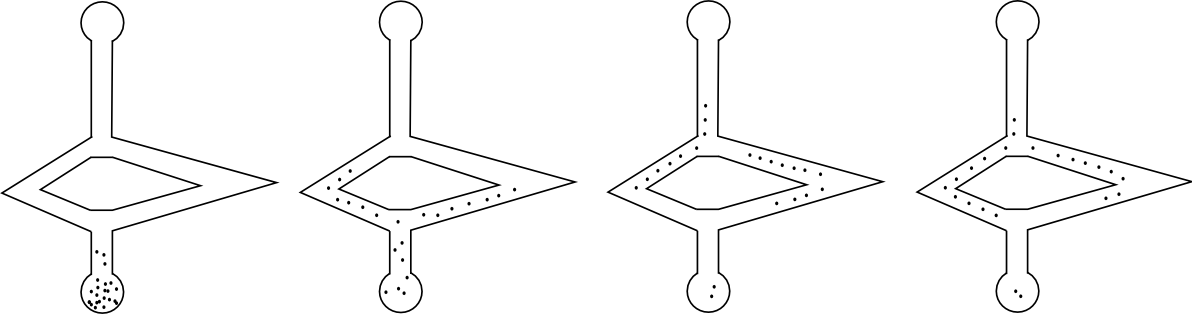
\includegraphics[width=\textwidth]{figs/ants.png}
	\caption{Ants finding the shortest path from their nest (bottom) to a food source (top). From left to right: The ants initially have equal preference for the left and the right branch, both going back and forth. As ants return faster on the shorter branch there will be more pheromones present on the short branch once a new ant arrives from the nest.}
	\label{fig:ants}
\end{figure}

Which solution to achieve a certain desired behavior is best depends on the resources that are available to the designer. We will now study a more elaborate problem for which many, more or less efficient, solutions exist.

\section{A roboticists' problem}
Imagine the following scenario. You are a robot in a maze-like environment such as a cluttered warehouse, hospital or office building. There is a chest full of gold coins hidden somewhere inside. Unfortunately, you don't have a map of the maze. In case you find the chest, you can only take a couple of coins at the time, and bring them to the exit door where your car is parked.

\begin{framed}
Think about a strategy that will allow you to harvest as many coins in the shortest time possible. Think about the cognitive and perception capabilities you would make use of. Now discuss alternative strategies, if you would not have these capabilities, i.e., what if you were blind, had no memory?
\end{framed}

These are exactly the same problems a robot would have. A robot is a mobile machine that has sensors and computation, which allows it to reason about its environment. Current robots are far from the capabilities that humans have, therefore it makes a lot of sense to think about what strategies \emph{you} would employ to solve a problem, if you were lacking important perception or computational capabilities.

Before we move forward discussing potential strategies for robots with impeded sensory systems, lets quickly consider an optimal strategy. You will need to explore the maze without entering any branch twice. You can use a technique known as \emph{depth-first search} to do this, but will need to be able to not only map, but also localize in the environment, e.g., by recognizing places and dead-reckoning on the map. Once you found the gold, you will need to plan the shortest path back to the exit, which you can then use to go back and forth until all the gold is harvested.

\section{Ratslife}\label{sec:ratslife}
Ratslife is a miniature robot maze competition developed by Olivier Michel from Cyberbotics S.A. The Ratslife environment can easily be created from LEGO bricks, card board or wood and the game can be played with any two mobile robots, preferably ones with the ability to identify markers in the environment. These include simple differential-wheel educational platforms with onboard cameras or even a smart-phone driven robot. Figure \ref{fig:ratslife} shows a simple sample environment that can be constructed from craft materials and can be used to teach the practical aspects of mobile robots and/or for competitions.


\begin{figure}
	\centering
		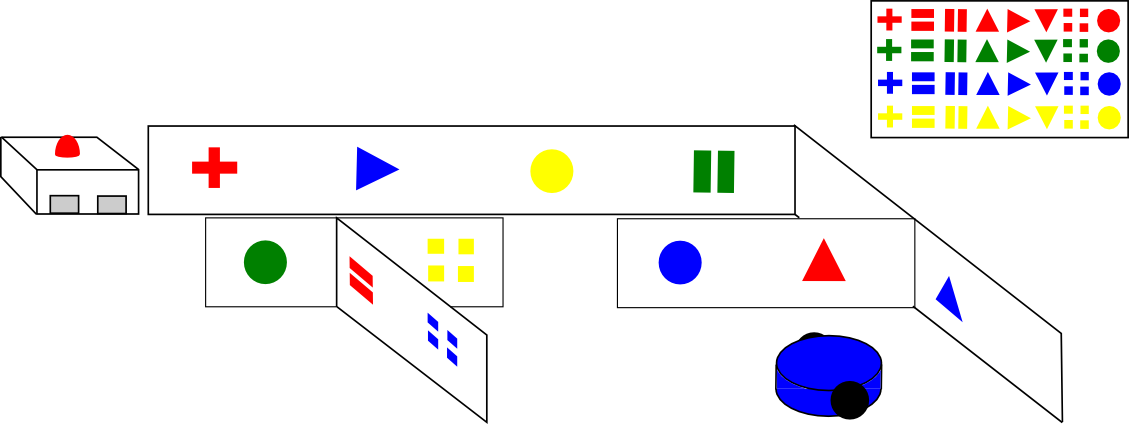
\includegraphics[width=\textwidth]{figs/ratslife.png}
	\caption{A simple maze made from cardboard, wood or Lego bricks with one ore more charging stations. Locations in the maze are marked with unique markers that can be recognized by a simple robot.}
	\label{fig:ratslife}
\end{figure}



In RatsLife, two miniature robots  compete on searching for four ``feeders'' that are hidden in  a maze. Once a robot reaches a feeder, it receives ``energy'' to go on for another 60s, and the feeder becomes temporarily unavailable. After a short while, the feeder becomes available again. The feeders can be either controlled by a referee who also takes care of time-keeping or constructed as part of a simple curriculum on electronics or mechatronics. 

It should be clear by now, how YOU would solve this tasks using your abilities, and you should also have thought about fall-back strategies in case some of your sensors are unavailable. Here are some possible algorithms for a robot, ordered after the capabilities that it provides:
\begin{itemize}
\item Imagine you have a robot that can only drive (actuation) and bounce of a wall. The resulting random walk will eventually let the robot reach a feeder. As the allowed time to do so is limited, it is likely that the robot's energy will soon deplete.
\item Now imagine a robot that has a sensor that let it estimate the distance from a wall. This could be a whisker, an infrared distance sensor, an ultra-sound distance sensor, or a laser range finder. The robot could now use this sensor to keep following a wall to its right. Using this strategy for solving the maze, it will eventually explore the entire maze except for islands inside of it.
\item Finally, think about a robot that could identify simple patterns using vision, has distance sensors to avoid walls, and an ``odometer'' to keep track of its wheel rotations. Using these capabilities, a potential winning strategy would be to explore the environment, identify markers in the environment using vision and use them to create a map of all feeder locations, calculate the shortest path from feeder to feeder and keep going back and forth between them. Strategy-wise, it might make sense to wait just in front of feeder and approach it only shortly before a robot runs out of power.
\end{itemize}

\section{Challenges of Mobile Autonomous Robots}

Being able to stitch sensor information together to a map of the environment just by counting your own steps and orienting yourselves using distinct features of the environment is known as Simultaneous Localization and Mapping (SLAM). The key challenge here is that the length of the steps you take are uncertain (a wheeled robot might slip or have slightly differently sized wheels, e.g.) and it is not possible to recognize places with 100\% accuracy (not even for a human). In order to be able to implement something like the last algorithm on a real robot, we will therefore need to understand

\begin{itemize}
\item How does a robot move? How does rotation of its wheels affects its position and speed in the world?
\item How do we have to control the wheel-speed in order to reach a desired position?
\item What sensors exist for a robot to perceive its own status and its environment?
\item How can we extract structured information from a vast amount of sensor data?
\item How can we localize in the world?
\item How can error be represented and how can we reason in the face of uncertainty?
\end{itemize}

In order to answer these questions, we will rely on trigonometry, linear algebra, and probability theory. Specific concepts that will be used throughout this book are basic trigonometry, matrix notation, Bayes' formula, and the concept of probability distributions. You will see that robotics is actually a great vehicle to add meaning to these concepts!


\section{Challenges of Autonomous Manipulation}
Think about the last time you worked with your hands. This includes typing on your keyboard, writing on a piece of paper, sewing a button onto a shirt, and using a hammer or a screwdriver. You will notice that these activities require a wide range of dexterity, that is the ability to manipulate objects with precision, a wide range of forces, and a wide range of sensorial capabilities. You will also notice that some tasks go beyond your capabilities, such as putting yarn through a hole in fabric, grasping a screw, or driving a nail into a piece of wood, but can be easily solved with the right tool.

So far, robotic hands are far from reaching the dexterity of a human hand. Yet, with the right tool (called ``end-effector'' in robotics speech) \index{End-effector} some tasks can be solved even better, that is faster and more precise, than by humans. As for solving a mobile robotics problem, manipulation problems require you to think about the right mix of reasoning and mechanism design. For example, grasping tiny parts might be impossible with tweezers, but really easy when using a sucking mechanism. Or, picking up a test tube that is hardly visible with the robots' sensors can be picked up almost blindly when using a funnel-like mechanism at your end-effector. Unfortunately, these tricks will most likely limit the versatility of your robot, requiring you to think about the problem and the users's need as a whole.

%\section{The first industrial robot ``Unimate"}
%Since the introduction of the first industrial robot ``Unimate'' in 1961, the robotics industry classically consists of static manipulators that perform repetitive tasks such as welding or part placement, as well as of remote controlled machines for exploring hazardous areas. Recent advances in sensor technology and artificial intelligence are quickly enabling a new kind of robotic system: robots that can take autonomous decisions. Most prominent example of this class of robots is iRobots ``Roomba'' vacuum cleaner that was introduced in 2002 and that uses a variation of algorithm \#1 above to solve the floor cleaning problem due to the lack of sophisticated sensors and computation. More recently, SLAM has found its ways into cars, university teams winning the DARPA Grand Challenge, Google's cars logging more than 140,000 miles, and Volkswagen presenting the first assisted driving system in 2011. Similarly, KIVA systems  successfully distributes mobile robots for automatic warehouses. These robots are still remote controlled and operate in constrained environments that provide them the ability to localize and reason on a simplified representation of the world - all items in the KIVA world are living on a grid. Novel sensors such as the xBox Kinect that provide 3D depth measurements at unprecedented low cost, increasingly capable and cheap computers, and a better understanding on how to reason about uncertainty will enable a large number of applications raising from autonomous warehouse helpers, home and elderly care, robotic toys and many other gimmicks straight from the Jetsons very soon.



\section*{Take-home lessons}
\begin{itemize}
\item How to best solve a problem is a function of the available sensing, actuation, computation and communication abilities of the available platform. Usually, there exist trade-offs that allow you to solve a problem using a minimal set of resources, but compromise performance such as speed, accuracy or reliability.
\item Robotics problems are different from problems in pure Artificial Intelligence, that do not deal with unreliable sensing or actuation.
\item The unreliability of sensors, actuators and communication links require a probabilistic notion of the system and reason with uncertainty.
\end{itemize}

\section*{Exercises}\small
\begin{enumerate}
\item What kind of sensors do you need to solve the ``Ratslife'' game? Think both about trivial and close-to-optimal approaches.
\item What devices in your home could be considered robots? Why and why not?
\item Which industries have been recently revolutionized by robotics? Into which industries were robots introduced first?
\item What sensors are you using when grasping an object? Enumerate them all. Which ones are absolutely necessary for good performance?
\item Think about robots vacuuming your floor or mowing your lawn? Do they use any planning? Why or why not?
\item What kind of sensors would you need in a car that drives completely autonomous? Think first about the kind of information that the car needs to be aware of and then discuss possible sensors that could capture this information.
\item Implement a simple line-following using a robot of your choice. How does the thickness of the line affect the sensor placement on the robot? How does its curvature affect the robot's speed?
\item Implement a maze solving algorithm that uses simple wall-following using a robot of your choice. How does the sensor geometry affect the robot's performance? What are the parameters that you find yourself tuning? 
\end{enumerate}\normalsize

%Robotics celebrated its 50th birthday in 2011, dating back to the first commercial robot in 1961 (the Unimate). In a ``Tonight show'' from the time, this robot did amazing things: its opening a bottle of beer, pouring it, putting a golf ball into the hole, and even conducting an orchestra. This robot does all what we expect a good robot to do: its dexterous, its accurate, and even creative. Since this robots appearance on the Tonight show more than 50 years have passed --- so how incredible must be the capabilities of today's robots and what must they be able to do?
%
%Interestingly, we just recently learned doing all the things demonstrated by Unimate autonomously. Unimate indeed did what was shown on TV, but all motions have been pre-programmed and the environment has been carefully staged.  Only the advent of cheap and powerful sensors and computation has recently enabled robots to detect an object by themselves, plan motions to it and grasp it. Yet, robotics is still far away from doing these tasks with human-like performance. Environments still need to be heavily staged for a robot to operate, and some objects are easier to work with than others. For example, ``Rollin' Justin'' is demonstrating skills very similar to those shown by the Unimate, but is able to perceive and reason about its environment:
%
%This works as follows: the robot perceives its environment with a sensor that generates 3D range data, such as stereo-vision, a sweeping laser scanner or an xbox Kinect. The robot creates a 3D representation of its environment that is relative to its own coordinate system. The robot now plans its motion using this 3D representation. This can be seen in the inset to the top right when the robot is manipulating items on the table. Detecting objects in the environment, matching them to their 3D model, and finding feasible grasp points are still major research challenges.
%
%The ``sense-plan-act'' paradigm, that is obtaining a 3D model of the world, planning therein, and consequently executing actions is not the final solution, however. Do humans really do this when performing complex manipulations? Rather not. Instead, we are relying on vision feedback or the sense of touch when performing a grasp. (Try to grasp an object after putting your hand on an ice block, temporarily impeding your sense of touch.)
%
%This class builds up on ``Introduction to Robotics'' and introduces current solutions to these problems. We will learn advanced concepts in robotic kinematics, such as car-like steering and inverse kinematics of high-DOF manipulators, feature recognition, RGB-D perception, visual servoing and SLAM. We will also learn to use state-of-the-art tools that allow you to model, visualize and control your robot. You will work with a 7-DOF manipulator arm both in simulation and using real hardware. The development environment consists of Ubuntu Linux, ROS and OpenCV that are available as VirtualBox. The real manipulator arm is available for experimentation in the lab. We will perform laboratory experiments - that can be mostly prepared and executed in simulation - that will introduce the tools and methods we are using and guide you toward an independent project.
%
%The class consists of homework assignments (experiments) and a team project. The final deliverable for the team project is a 3 page (5 pages) for undergraduates (graduate students). Your team project needs to articulate a hypothesis (what do you want to show?) that is validated experimentally on physical hardware. In order to prepare you for this, each laboratory exercise will require analys of experimental data rather than submission of code.
\chapter{Locomotion and Manipulation}\label{chap:locomotion}
Autonomous robots are systems that sense, actuate, compute, and communicate. Actuation, the focus of this chapter, is the ability of the robot to move and to manipulate the world. Specifically, we differentiate between locomotion\index{Locomotion} as the ability of the robot to move and manipulation\index{Manipulation} as the ability to move objects in the environment of the robot. Both activities are closely related: during locomotion the robot uses its motors to exert forces on its environment (ground, water or air) to move itself; during manipulation it uses motors to exert forces on objects to move them relative to the environment. This might not even require different motors. Insects are good examples for this: both can use their 6 legs not only for locomotion, but also for picking up and manipulating objects. The goals of this chapter are
\begin{itemize}
\item introduce the concepts of locomotion, manipulation and their duality
\item explain static vs.\ dynamic stability
\item introduce the concept of reference frames and ``degrees-of-freedom''
\item and introduce forward kinematics of static arms.
\end{itemize}

\section{Locomotion and Manipulation Examples}
Locomotion includes very different concepts of motion including rolling, walking, running, jumping, sliding (undulatory locomotion), crawling, climbing, swimming, and flying. Although walking, running, jumping, crawling and climbing seem to be very similar concepts at first sight, they are drastically different in terms of energy consumption, kinematics, stability, and capabilities required by the robot that implements them. The way in which the individual parts of a robot can move with respect to each other and the environment is called the \emph{kinematics}\index{Kinematics} of the robot. Kinematics are only concerned with the position and speed (first derivative of position) of those parts, but not its \emph{dynamics}, which include acceleration (second derivative of position) and jerk (third derivative of position).
%Examples include:
%
%\begin{itemize}
%\item Walking: Honda's ASIMO (2-legged) and Sony's AIBO.
%\item Running: Boston Dynamics' Athlete robot (2-legged) Big Dog (4-legged).
%\item Jumping: EPFL's Micro-gliders
%\item Sliding:  EPFL's Salamandra robot
%\item Crawling: Harvard's mesh worm
%\item Climbing: Stanford's StickyBot
%\item Swimming: FESTO's AquaJelly, MIT's AMOUR robot, and various robotic fish.
%\end{itemize}

Although the above taxonomy serves as an initial rough classification, the definitions are loose and ambiguous: for example, ``swimming'' can be done using many different forms of propulsion systems. Similarly, a sliding motion on the ground might result into swimming with only few modifications. Commercially, the most dominant form of locomotion is rolling. This is due to the fact that rolling provides by far the most efficient energy-speed ratio (Figure \ref{fig:todd}), making the invention of the wheel one of the greatest technological breakthroughs in history. Consequently, humans have modified their environment to have smooth surfaces of large extent such as the road network, but also warehouse and residential floors. In contrast, evolution has not evolved a single animal with wheel-like actuators.

\begin{figure}
	\centering
		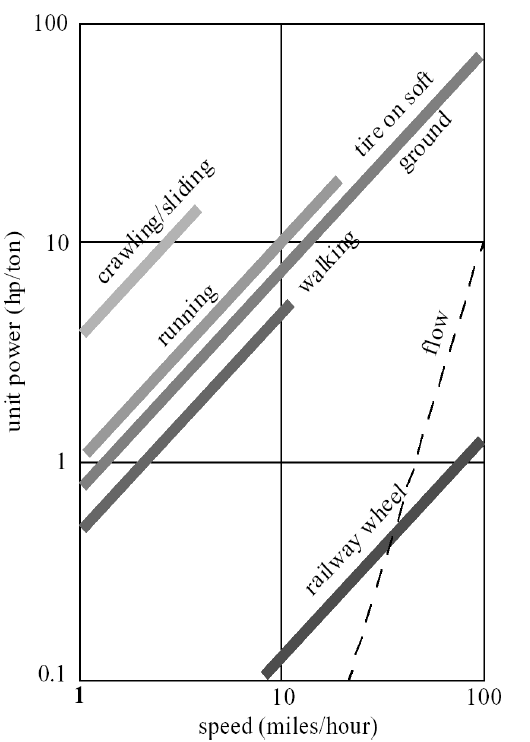
\includegraphics[width=0.8\textwidth]{figs/todd85.png}
	\caption{Power consumption vs.\ speed for various means of locomotion. From: Todd, D.J. Walking Machines: An Introduction to Legged robots. London, Kogan Page Ltd., 1985}
	\label{fig:todd}
\end{figure}


\begin{framed}Can you find examples of robots from the above categories? Identify the different types of actuators that are used in them.
\end{framed}

Due to the dominance of rolling robots, the electric motor is among the most popular actuators. Except for the stepper motor, which uses large electromagnets to rotate an internal spindle by a few degrees every time, the physics of the electrical motor requires it to revolve at very high speeds (multiple thousand rotations per minute). Therefore, motors are almost always used in conjunction with gears to reduce the speed and increase the torque, that is the force that the motor can exert to rotate an axis. In order to be able to measure the number of revolutions and the axis' position, motors are also often combined with rotary encoders. Motors that combine an electric motor with a gear-box, encoder, and controller to move toward desired position are known as servo motors, and are popular among hobbyists. Another popular class of actuator, in particular for legged robots, are linear actuators, that might exist in electric, pneumatic or hydraulic form. Finally, there exist a wide array of specialty actuators such as Shape-Memory Alloys, Electroactive Polymers or Piezo-elements, which often allow for extreme miniaturization, but do not provide attractive energy-to-force ratios and are difficult to control.

Most actuators (and mechanisms) capable of locomotion can also be used for manipulation with only minor modifications. Most industrial manipulators consist of a chain of rotary actuators that are connected by links. Most industrial robots have six or more independently rotating axes. We will see why further down below. Modern industrial manipulators have the ability to not only control the position of each of its joints, but precisely control the torque and force at each individual joint, making the arm arbitrary compliant, which is the inverse of stiffness in a mechanical sense. For dexterous manipulation a robot does not only need an arm, but also a gripper or hand. Grasping is a hard problem and deserves its own chapter. 

%This lecture focuses on the kinematics of simple mechanisms. Understanding the duality between locomotion and manipulation is important, however, to better introduce (and understand) concepts such as reference frames and forward kinematics.

\section{Static and Dynamic Stability}\label{sec:stability}
A fundamental difference between locomotion mechanisms is whether they are statically or dynamically stable\index{Static stability}\index{Dynamic Stability}. A statically stable mechanism will not fall even when all of its joints freeze (Figure \ref{fig:stability}, left). A dynamically stable robot instead requires constant motion to prevent it from falling. Technically, stability requires the robot to keep it's center of mass to fall within the polygon spanned by its ground-contact points. For example a quadruped robot's feet span a rectangle. Once such a robot lifts one of its feet, this rectangle becomes a triangle. If the projection of the center of mass of the robot along the direction of gravity is outside of this triangle, the robot will fall. A dynamically stable robot can overcome this problem by changing its configuration so rapidly that a fall is prevented. An example of a purely dynamically stable robot is an inverted pendulum on a cart  (Figure \ref{fig:stability}, middle). Such a robot has no statically stable configurations and needs to keep moving all the time to keep the pendulum upright. While dynamic stability is desirable for high-speed, agile motions, robots should be designed so that they can easily switch into a statically stable configuration (Figure \ref{fig:stability}, right). 

\begin{figure}
	\centering
		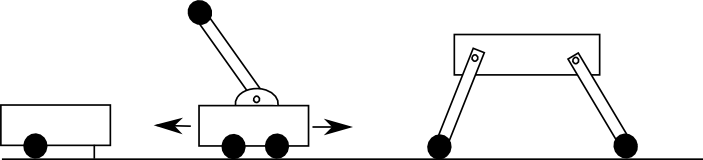
\includegraphics[width=\textwidth]{figs/stability.png}
	\caption{From left to right: statically stable robot. Dynamically stable inverted pendulum robot. Static and dynamically stable robot (depending on configuration).}
	\label{fig:stability}
\end{figure}

An example of a robot that has both statically and dynamically stable configurations is a quadruped (``four legs'') runner. Unlike walking, a running robot will always have two legs in the air and alternate between them faster than the robot could fall in either direction. Although statically stable walking is possible with only 4 legs, most animals (and robots) require 6 legs for statically stable walking and use dynamically stable gaits (such as galloping) when they have four legs. Six legs allow the animal to move three legs at a time while the three other legs maintain a stable pose.


\section{Degrees-of-Freedom}\label{sec:dof}
The concept of \emph{degrees-of-freedom}\index{Degree of freedom}, often abbreviated as DOF, is important for defining the possible positions and orientations a robot can reach. An object in the physical world can have up to six degrees of freedom, namely forward/backward, sideways, and up/down as well as rotations around those axes. How many of those directions a robot can move in is not always intuitive and requires more rigorous mathematical treatment (Chapter \ref{chap:kinematics}). The goal of this chapter is to introduce the degrees of freedom of standard mechanisms that are recurrent in robot design such as wheels or simple arms. For wheeled platforms, the degrees-of-freedom are defined by the types of wheels used and their orientation. Common wheel types are listed in Table \ref{tab:wheels}.

\begin{table}
\begin{tabular}{p{2.8cm}p{3cm}p{4cm}}
\hline
Wheel type & Example & Degrees-of-Freedom\\
\hline
Standard 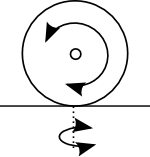
\includegraphics[width=2.5cm]{figs/wheeltype_standard.png} &	Front-wheel of a wheelbarrow	& Two
\begin{compactitem}
\item Rotation around the wheel axle
\item Rotation around its contact point with the ground
\end{compactitem}\\
\hline
Caster wheel	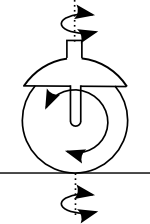
\includegraphics[width=2.5cm]{figs/wheeltype_caster.png}& Office chair & Three
\begin{compactitem}
\item Rotation around the wheel axle
\item Rotation around its contact point with the ground
\item Rotation around the caster axis
\end{compactitem}\\
\hline
Swedish wheel 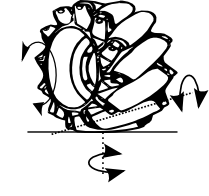
\includegraphics[width=2.5cm]{figs/wheeltype_swedish.png}& Standard wheel with non-actuated rollers around its circumference& Three
\begin{compactitem}
\item Rotation around the wheel axle
\item Rotation around its contact point with the ground
\item Rotation around the roller axles
\end{compactitem}\\
\hline
Spherical wheel 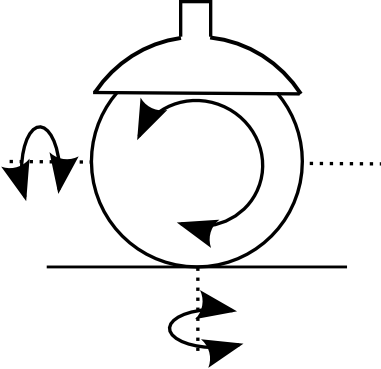
\includegraphics[width=2.5cm]{figs/wheeltype_spherical.png}& Ball Bearing & Three
\begin{compactitem}
\item Rotation in any direction
\item Rotation around its contact point
\end{compactitem}\\
\hline
\end{tabular}
\caption{Different types of wheels and their degrees of freedom.\label{tab:wheels}}
\end{table}

Only robots that use exclusively wheels with three degrees-of-freedom (3-DOF wheels) will be able to freely move on a plane. All other robots will have \emph{kinematic constraints}\index{Kinematic constraints} that prevent them from reaching every possible point at every possible orientation. A good analogue are figures on a chess-board. For example, a knight can reach every cell on a chess-board but might require multiple moves to do so. This is similar to a car, which can parallel park using back-and-forth motions. Instead, a bishop can only reach either black or white fields on the board. This is equivalent to a robot, which has non-steerable standard wheels and can only reach a sub-set of the environment without skidding.

Similar reasoning applies to aerial and underwater robots. Here, the position of the robot is affected by the position and orientation of thrusters, either in the form of jets or propellers, mounted on the robot. Things become complicated quickly, however, as the dynamics of the system are subject to fluid- and aerodynamic effects, which also change as a function of size of the robot. This book will not go into the details of flying and swimming robots, but the general principles of localization and planning will be applicable to them as well.

\begin{framed}Think about possible wheel, propeller and thruster configurations. Don't limit yourself to robots, but consider also street and aerial vehicles and be creative --- if you can think about a setup that makes sense, i.e., allows for reasonable mobility --- somebody will already have built it and analyzed it. What are the advantages and disadvantages of each?
\end{framed}

For manipulating arms, degrees of freedom usually refer to the positions and orientations, i.e., rotations around the primary axes, the end-effector can reach. As a rule of thumb, each joint usually adds a degree of freedom unless they are redundant, that is, moving in the same direction. Figure \ref{fig:basickinematics} shows a series of manipulators operating in the $x-y$-plane. By this, the degrees of freedom of the end-effector are limited to moving along the $x$ and $y$-axis as well as rotating around the $z-$axis. Therefore adding additional joints does not increase the degrees of freedom unless they allow the robot to also rotate around the $x$ and $y$ axis. 

An exact definition of the number of degrees of freedom is tricky and requires deriving analytical expressions for the end-effector position and orientation, which will be subject to Chapter \ref{chap:kinematics}.

\begin{figure}
	\centering
		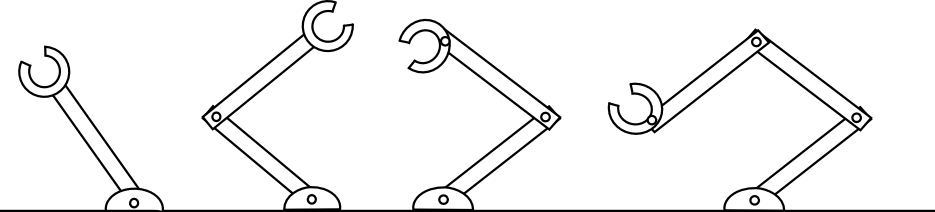
\includegraphics[width=\textwidth]{figs/basickinematics.png}
	\caption{From left to right: Manipulators with one, two, three and three DOF. The degrees of freedom of moving in a plane are $x$ and $y$ position, as well as rotation around the $z$ axis.}
	\label{fig:basickinematics}
\end{figure}

Choosing the ``right'' kinematics is a trade-off between mechanical complexity, maneuverability, achievable precision, cost, and ease of control. The very popular differential-wheel drive consisting of two independently controlled wheels that share a common axis such as on the iRobot Roomba is cheap, highly maneuverable and easy to control, but makes it hard to drive in a straight line. This requires both motors to turn at the exact same speed and both wheels to have the exact same diameter, which is hard to achieve in practice. This problem is solved well by car-like steering mechanisms, but they have poor maneuverability and are difficult to control (think parallel-parking).

\section*{Exercises}
\begin{enumerate}
\item What are the degrees of freedom of a lawnmower? Why are you still able to mow your entire lawn?
\item Is a car statically or dynamically stable? What about a Segway?
\item What are the degrees of freedom of an office chair with all caster-wheels?
\item What are the maximum degrees of freedom for objects driving on the plane?
\item What are the maximum degrees of freedom for objects in a 3D coordinate system?
\end{enumerate}

\section*{Take-home lessons}

\begin{itemize}
\item In order to do planning for a robot, you need to understand how its control parameters map to actions in the physical world.
\item The kinematics of a robot are fully defined by the position and orientation of its wheels, joints and links no matter whether it swims, flys, crawls or drives.
\item Many robotic systems cannot be fully understand by considering kinematics alone, but require you to model their dynamics as well. This book will be limited to modeling kinematics, which is sufficient for low-speed, mobile robots and arms.
\end{itemize} 
\chapter{Forward and Inverse Kinematics}\label{chap:kinematics}
In order to plan a robot's movements, we have to understand the relationship between the actuators that we can control and the robot's resulting position in the environment. For static arms, this is rather straightforward: if we know the position/angle of each joint, we can calculate the position of its end-effectors using trigonometry. This process is known as \emph{forward kinematics}. \index{Forward Kinematics} If we want to calculate the position each joint needs to be at, we need to invert this relationship. This is known as inverse kinematics. \index{Inverse Kinematics}

The goals of this chapter are:

\begin{itemize}
\item introduce coordinate systems and their transformations,
\item to introduce the forward kinematics of mobile robots and simple arms,
\item show how solutions for the inverse kinematics for both static and mobile robots can be derived,
\item provide an intuition on the relationship between inverse kinematics and path-planning.
\end{itemize}

\section{Coordinate Systems and Frames of Reference}\label{sec:coordsystems}
\screencast{http://youtu.be/klBJi-MEeNQ}{coordinatesystem}
Every robot assumes a position in the real world that can be described by its position (x, y and z) and orientation (pitch, yaw and roll) along the three major axes of a Cartesian Coordinate system (See also Section \ref{sec:dof}, ``Degrees of freedom''). Such a coordinate system is shown in Figure \ref{fig:coordinatesystem}. Note that the directions and orientations of the coordinate axes are arbitrary. This books uses the ``right hand rules'', which are illustrated in Figure \ref{fig:coordinatesystem} to determine axes labels and directions throughout.

\begin{figure}
	\centering
		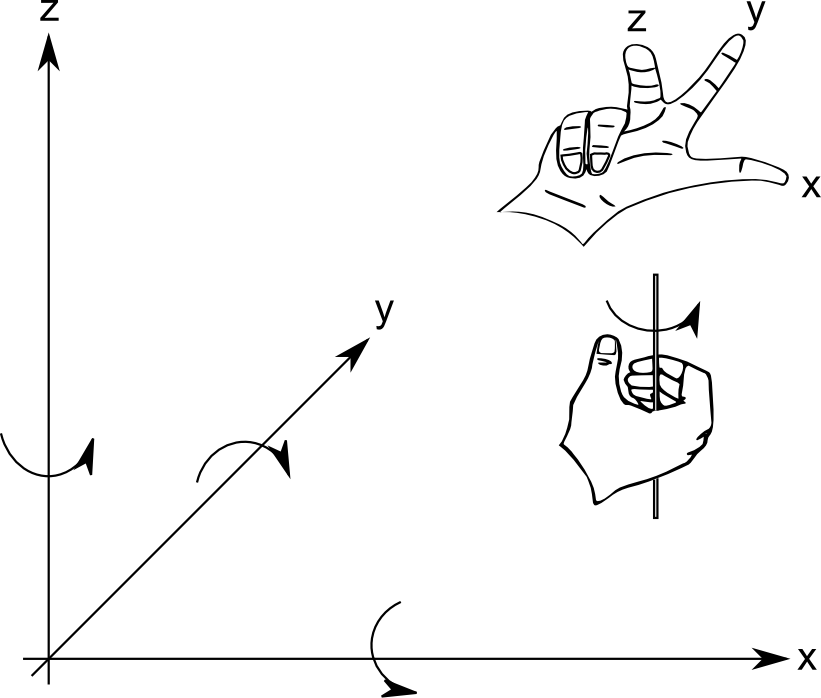
\includegraphics[width=0.8\textwidth]{figs/coordinatesystem}
	\caption{A coordinate system indicating the direction of the coordinate axes and rotation around them. These directions have been derived using the right-hand rules.}
	\label{fig:coordinatesystem}
\end{figure}

Defining all three position axes and orientations might be cumbersome. What level of detail we care about, where the origin of this coordinate system is, and even what kind of coordinate system we chose, depends on the specific application. For example, a simple mobile robot would typically require a representation with respect to a room, a building, or the earth's coordinate system (given by the longitude and latitude of each point on the earth), whereas a static manipulator usually has the origin of its coordinate system at it's base. More complicated systems, such as mobile manipulators or multi-legged robots, make life much easier by defining multiple coordinate systems, e.g.\ one for each leg and one that describes the position of the robot in the world frame. These local coordinate systems are known as \emph{Frames of Reference}\index{Frame of Reference}. 
An example of two nested coordinate systems is shown in Figure \ref{fig:nestedcoords}. In this example, a robot located at the origin of $x',y'$ and $z'$ might plan its motions in its own reference frame, which can then be expressed in the coordinate system $x$, $y$ and $z$ by performing a translation and a rotation as we will later see. 

Depending on it's degrees-of-freedom, that is the number of independent translations and rotations a robot can achieve in Cartesian space, it is also customary to ignore components of position and orientation that remain constant. For example a simple floor-cleaning robot's pose might be completely defined by it's $x$ and $y$ coordinates in a room as well as its orientation, i.e.\ its rotation around the $z$-axis. 


\begin{figure}
	\centering
		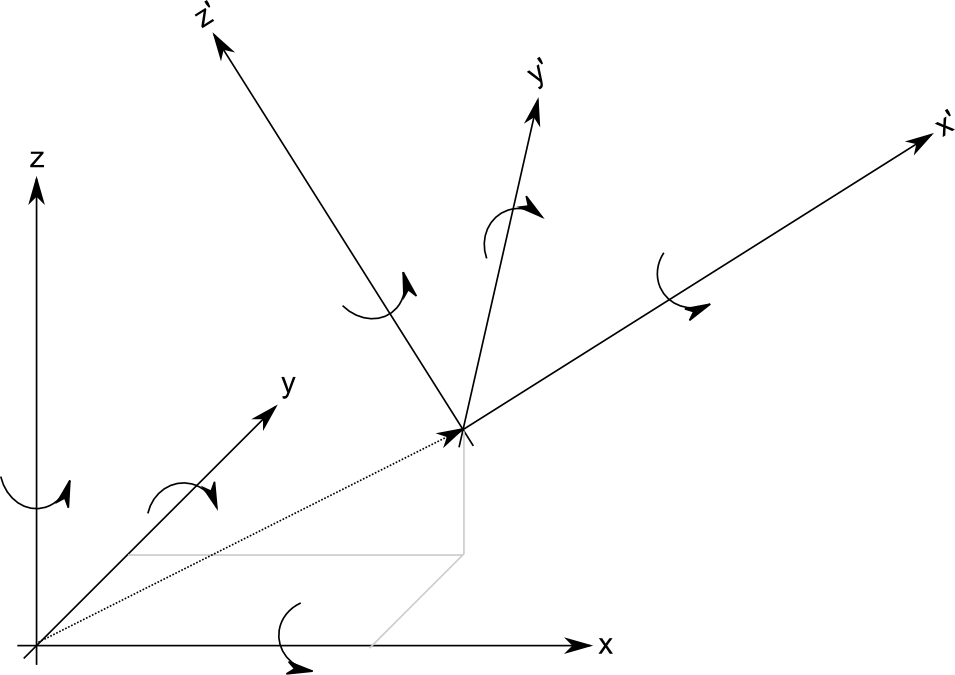
\includegraphics[width=\textwidth]{figs/frameofreference.png}
	\caption{Two nested coordinate systems (frames of reference).}
	\label{fig:nestedcoords}
\end{figure}

\subsection{Matrix notation}
Given some kind of fixed coordinate system, we can describe the \emph{position} of a robot's end-effector by a $3x1$ position vector. As there can be many coordinate systems defined on a robot and the environment, we identify the coordinate system a point relates to by a preceeding super-script, e.g., $ ^AP$ to indicate that point $P$ is in coordinate system $\{A\}$. Each point consists of three elements $ ^AP=[p_x p_y p_z]^T$.


\screencast{http://youtu.be/QdHO_9M8-UI}{frameofreference}
As we know, not only the position of the robot is important, but also its orientation. In order to describe the orientation of a point, we will attach a coordinate system to it. Let $ \hat{X}_B, \hat{Y}_B$ and $ \hat{Z}_B$ be unit vectors that correspond to the principal axes of a coordinate system $\{B\}$. When expressed in coordinate system $\{A\}$, they are denoted $^A\hat{X}_B, ^A\hat{Y}_B$ and $ ^A\hat{Z}_B$. In order to express a vector that is given in one coordinate system in another, we need to project each of its components to the unit vectors that span the target coordinate system. For example

\begin{equation}\label{eq:projection}
^A\hat{X}_B=(\hat{X}_B\cdot\hat{X}_A, \hat{X}_B\cdot\hat{Y}_A,\hat{X}_B\cdot\hat{Z}_A)^T
\end{equation}
consists of the projections of $\hat{X}_B$ onto $\hat{X}_A$, $\hat{Y}_A$ and $\hat{Z}_A$. Here,  $|\cdot|$ denotes the scalar product (also known as dot or inner product).  Note that all vectors in (\ref{eq:projection}) are unit vectors, i.e. their length is one. By definition of the scalar product, $A\cdot B=\|A\|\|B\|\cos \alpha=\cos \alpha$, indeed reduces the projection of $\hat{X}_B$ onto the unit vectors of $\{A\}$. This projection is illustrated in Figure \ref{fig:projection}.

\begin{figure}
	\centering
		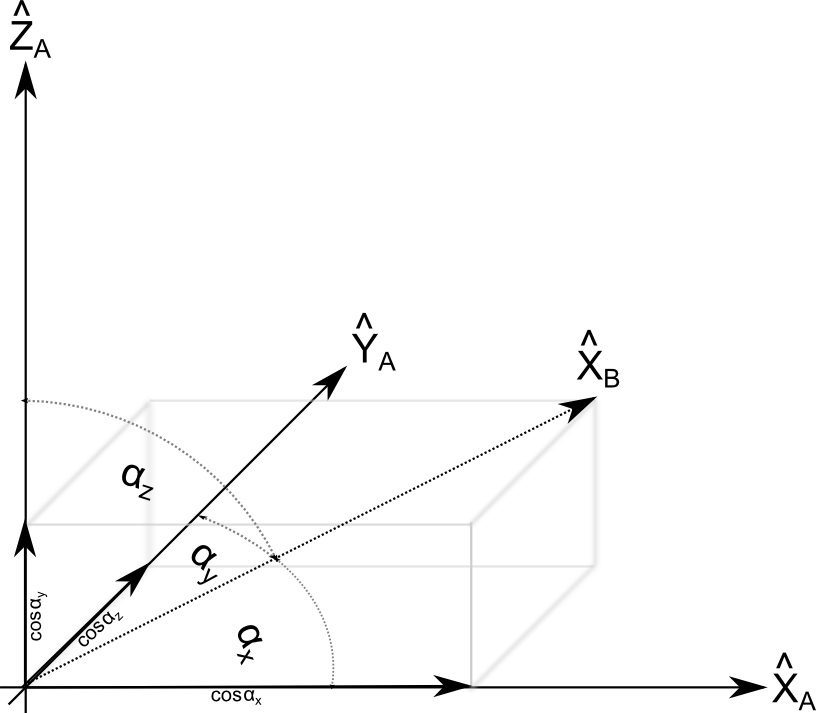
\includegraphics[width=\textwidth]{figs/projection.png}
	\caption{The projection of the unit vector $\hat{X}_B$ onto the unit vectors that span coordinate system $\{A\}$. As all vectors are unit vectors, $A\cdot B=\|A\|\|B\|\cos \alpha=\cos \alpha$. For clarity, only $\hat{X}_B$ of coordinate system $\{B\}$ is shown. }
	\label{fig:projection}
\end{figure}

We can now do this for all three vectors that span coordinate system $\{B\}$ and stack these three vectors together into a 3x3 matrix to obtain the rotation matrix
%
\begin{equation}
^A_BR=[^A\hat{X}_B \quad ^A\hat{Y}_B \quad ^A\hat{Z}_B]
\end{equation}
%
which describes $\{B\}$ relative to $\{A\}$. It is important to note that all columns in $ ^A_BR$ are unit vectors, so that the rotation matrix is orthogonal. This is important as this allows us to easily obtain the inverse of $ ^A_BR$ as $ ^A_BR^T$ or
$ ^B_AR=^A_BR^T$. 

%http://www.youtube.com/watch?v=CxsF2xV78RQ

We have now established how to express the orientation of a coordinate system using a rotation matrix. Usually, coordinate systems don't lie on top of each other, but are also displaced from each other. 
Together, position and orientation is known as a \emph{frame},\index{Frame} which is a set of four vectors, one for the position and three for the orientation, and we can write
%
\begin{equation}
\{B\}=\{^A_BR, ^AP\}
\end{equation}
%
to describe the coordinate frame $\{B\}$ with respect to $\{A\}$ using a vector $^AP$ and a rotation matrix $^A_BR$. Robots usually have many such frames defined along their bodies.

\subsection{Mapping from one frame to another}
\screencast{http://youtu.be/NsiJNvsuO3s}{rotationmatrix}
Having introduced the concept of frames, we need the ability to map coordinates in one frame to coordinates in another frame. For example, lets consider frame $\{B\}$ having the same orientation as frame $\{A\}$ and sitting at location $^AP$ in space. As the orientation of both frames is the same, we can express a point $ ^BQ$ in frame $\{A\}$ as
%
\begin{equation}
^AQ=^BQ+^AP
\end{equation}
%
Actually, adding two vectors that are in different reference frames, i.e., $ ^BQ+^AP$, is only possible if both of them have the same orientation. We can, however, convert from one reference frame to the other using the rotation matrix:

\begin{equation}
^AP=^A_BR^BP
\end{equation}
%
and therefore solve the mapping problem regardless of the orientation of $\{A\}$ to $\{B\}$:
\begin{equation}
^AQ=^A_BR^BQ+^AP
\end{equation}
Using this notation, we can see that leading subscripts cancel the leading superscripts of the following vector/rotation matrix. Whereas we have now a solution to transfer a point from one frame of reference to another by combining a rotation and a translation, it would be more appealing to write something like that:
\begin{equation}
^AQ=^A_BT^BQ
\end{equation}
In order to do this, we need to introduce a 4x1 position vector such that
\begin{equation}
\left[\begin{array}{c}^AQ\\\end{array}\right]=\left[\begin{array}{ccc|c} & ^A_BR & & ^AP \\\hline 0 & 0 & 0 & 1\end{array}\right]\left[\begin{array}{c}^BQ\\1\end{array}\right]
\end{equation}
and $^A_BT$ is a 4x4 matrix.  Note that the added `1`s and $ [0 0 0 1]$ do not affect the other entries in the matrix during matrix multiplication. A 4x4 matrix of this form is called a \emph{homogenous transform}.\index{Homogenous Transform}

The inverse of an homogeneous transform can be constructed by inverting rotation and translation part independently, leading to
\begin{equation}
\left[\begin{array}{ccc|c} & ^A_BR & & ^AP \\\hline 0 & 0 & 0 & 1\end{array}\right]^{-1}=
\left[\begin{array}{ccc|c} & ^A_BR^T & & -^A_B{R^T}{^AP} \\\hline 0 & 0 & 0 & 1\end{array}\right]
\end{equation}

We have now established a convenient notation to convert points from one coordinate system to another. There are many possible ways this can be done, in particular how rotation can be represented (see below), but all can be converted from one into the other. 

\subsection{Transformation arithmetic}
Transformations can be combined: consider for example an arm with two links, reference frame $\{A\}$ at the base, $ \{B\} $ at its first joint, and $\{C\}$ at its end-effector. Given the transforms $ ^B_CT$ and $ ^A_BT$, we can write
\begin{equation}
^AP=^A_BT^B_CT^CP=^A_CT^CP
\end{equation}
to convert a point in the reference frame of the end-effector to that of its base. As this works for rotation and translation operators independently, we can construct $ ^A_CT$ as
\begin{equation}
^A_CT=\left[\begin{array}{ccc|c} & ^A_BR^B_CR & & ^A_BR^BP_C +^AP_B \\\hline 0 & 0 & 0 & 1\end{array}\right]
\end{equation}
%
where $ ^AP_B$ and $ ^BP_C$ are the translations from $\{A\}$ to $\{B\}$ and from $ \{B\}$ to $\{C\}$, respectively.

\subsection{Other representations for orientation}
So far, we have represented orientation by a 3x3 matrix who's column vectors are orthogononal  unit vectors describing the orientation of a coordinate system. Orientation is therefore represented with nine different values. We chose this representation mainly because it is the most intuitive to explain and is derived from simple geometry.

In fact, three values are sufficient. This becomes clear when considering that orthogonality (dot product of all columns is zero) and vector length (each vector must have length 1) impose six constraints on the nine values in the rotation matrix. Indeed, an orientation can be represented about a rotation by certain angles around the $x$, the $y$, and the $z$-axis of the reference coordinate system. This is known as the $X-Y-Z$ fixed angels notation.\index{Fixed angel notation} Mathematically, this can be represented by a rotation matrix of the form
\begin{equation}
\tiny
^A_BR_{XYZ}(\gamma,\beta,\alpha)=\left[\begin{array}{ccc}cos\alpha & -sin\alpha & 0\\sin\alpha & \cos\alpha & 0\\0 & 0 & 1\end{array}\right]\left[\begin{array}{ccc}cos\beta& 0 & sin\beta\\0 & 1 & 0\\-sin\beta & 0 & cos\beta\end{array}\right]\left[\begin{array}{ccc}1 & 0 & 0 \\ 0 & cos\gamma & -sin\gamma\\0 & sin\gamma & cos\gamma\end{array}\right]
\end{equation}

While the $X-Y-Z$ fixed angels approach expresses a coordinate frame using rotations with respect to the original coordinate frame, say $\{A\}$, another possible description is to start with a coordinate frame $\{B\}$ that is coincident with frame $\{A\}$, then rotate around the Z-axis with angle $ \alpha$, then the Y-axis with angle $ \beta$ and finally around the X-axis with angle $ \gamma$. This representation is called Z-Y-X Euler angels.\index{Euler angels}

It is important to know about the subtle differences between the different available transformations as there is no ``right'' or ``wrong'', but different manufacturers use different conventions. Among these, the preferred representation for computational and stability reasons are \emph{Quaternions}\index{Quaternion}. A quaternion is a 4-tuple that extends the complex numbers with very general applications in mathematics and representing orientation and rotation in particular. The basic idea is that each rotation can be represented as a rotation around a single axis (a vector in space) by a specific angle. Given such an axis $ \hat{K}=[k_x k_y k_z]^T$ and an angle $ \theta$, one can calculate the so-called Euler parameters\index{Euler parameters} or unit quaternion\index{unit quaternion}:

\begin{eqnarray}
\epsilon_1=k_x sin \frac{\theta}{2}\\
\epsilon_2=k_y sin \frac{\theta}{2}\\
\epsilon_3=k_z sin \frac{\theta}{2}\\
\epsilon_4=cos\frac{\theta}{2}
\end{eqnarray}

These four quantities are constrained by the relationship
\begin{equation}
\epsilon_1^2+\epsilon_2^2+\epsilon_3^2+\epsilon_4^2=1
\end{equation}
which might be visualized by a point on a unit hyper-sphere. Transformations are represented by \emph{dual quaternions}\index{Dual quaternion}, one for the translation and one for the rotation. Dual quaternions can again easily be converted into homogenous transformation matrices.

\section{Forward kinematics of a Manipulator Arm}

\begin{figure}[!htb]%{L}{0.3\textwidth}
  \begin{center}
    \includegraphics[width=0.27\textwidth]{figs/fwk2dofarm}
  \end{center}
  \caption{A simple 2-DOF arm.\label{fig:fwk2dofarm}}
\end{figure}

Imagine you have a robot arm made out of two links and two joints that is mounted to a table. Let the length of the first link be $l_1$ and the length of the second link be $ l_2$. You could specify the position of the link closer to the table by the angle $ \alpha$ and the angle of the second link relative to the first link using the angle $ \beta$. Suitable conventions and coordinate systems are shown in Figure \ref{fig:fwk2dofarm}

We can now calculate the position of the joint between the first and the second link using simple trigonometry:

\begin{eqnarray}\label{eq:cosxl1}
x_1 &=&\cos \alpha l_1\\
y_1 &=&\sin \alpha l_1
\end{eqnarray}

Similarly, the position of the end-effector is given by

\begin{eqnarray}
x_2&=&\cos(\alpha+\beta)l_2+x_1\\
y_2&=&\sin(\alpha+\beta)l_2+z_1
\end{eqnarray}
%
or together, the position of the end-effector $(x,y)$ is given by

\begin{eqnarray}\label{eq:cosx}
x&=&\cos(\alpha+\beta)l_2+\cos\alpha l_1\\
y&=&\sin(\alpha+\beta)l_2+\sin\alpha l_1
\end{eqnarray}

The above equations are the kinematic equations of this robot as they relate its control parameters $ \alpha$ and $ \beta$ to the position of its end-effector given in the local coordinate system spanned by $ x$ and $ z$. Note that both $\alpha$ and $\beta$ shown in the figure are positive: Both links rotate around the z-axis. Using the right-hand rule, the direction of positive angles is defined to be counter-clockwise. 

The \emph{configuration space} \index{Configuration space}\index{C-Space (Configuration space)}, i.e., the set of angles each actuator can be set to, of this robot is given by $ \frac{-\pi}{2}<\alpha<\frac{\pi}{2}$ as it is not supposed to run into the table, and $ -\pi < \beta < \pi$. The configuration space is given with respect to the robot's joints and allows us to calculate the \emph{workspace}\index{Workspace} of the robot, i.e., the physical space it can move to, using the forward kinematic equations. This terminology will be identical for mobile robots. An example of configuration and work-space for both a manipulator and a mobile robot is shown in Figure \ref{fig:holonomy}.

The orientation of the arm's end-effector is given by $\alpha+\beta$. We can now write down  a transformation that includes a rotation around the z-axis
\begin{equation}
\label{eq:2armtrans}
\left(\begin{array}{llll}cos_{\alpha\beta} & -sin_{\alpha\beta} &  0 & \cos_{\alpha\beta}l_2+\cos\alpha l_1\\
                        sin_{\alpha\beta} & cos_{\alpha\beta} & 0 & \sin_{\alpha\beta}l_2+\sin\alpha l_1\\
												0 & 0 & 1 & 0\\
												0 & 0 & 0 & 1\end{array}\right)
\end{equation}
The notation $sin_{\alpha\beta}$ and $cos_{\alpha\beta}$ are short-hand for $sin(\alpha+\beta)$ and $cos(\alpha+\beta)$, respectively.


\section{Inverse Kinematics of a Simple Manipulator Arm}
We will now look at the kinematics of a 2-link arm that we introduced earlier. We need to solve the equations determining the robot's forward kinematics by solving for $ \alpha$ and $ \beta$. This is tricky, however, as we have to deal with complicated trigonometric expressions.

To get an intuition, assume there to be only one link, $l_1$.  Solving (\ref{eq:cosxl1}) for $\alpha$ yields actually two solutions $\left[\cos^{-1}\frac{x_1}{l_1},-\cos^{-1}\frac{x_1}{l_1}\right]$, as cosine is symmetric for positive and negative values. Indeed, for any possible position on the $x-axis$ ranging from $-l_1$ to $l_1$, there exist two solutions. One with the arm above the table, one with the arm within the table. (At the extremes of the workspace, both solutions are the same.)

%\begin{verbatim}
%sol = Solve[Sin[a + b] + Sin[a] == y
%              && Cos[a + b] + Cos[a] == x,
%             {a, b}];
%min = sol /. {x -> 1, y -> 1}
%\end{verbatim}

Solving for both degrees of freedom actually yields eight solutions, of which only two are feasible:

\begin{equation}
\alpha \rightarrow \cos^{-1}\left(\frac{x^2 y + y^3 - \sqrt{4 x^4 - x^6 + 4 x^2 y^2 - 2 x^4 y^2 - x^2 y^4}}{2 (x^2 + y^2)}\right)
\end{equation}
and
\begin{equation}
\beta \rightarrow -\cos^{-1}\left(1/2(-2+x^2+y^2)\right)
\end{equation}

What will drastically simplify this problem, is to not only specificy the desired position, but also the orientation of the end-effector. In this case, a desired pose can be specified by
\begin{equation}
\left(
\begin{array}{cccc}
cos\phi & -sin\phi & 0 & x\\
sin\phi & cos\phi & 0 & y\\
0 & 0 & 1 & 0\\
0 & 0 & 0 & 1
\end{array}
\right)
\end{equation}
A solution can now be found by simply equating the individual entries of the transformation (\ref{eq:2armtrans}) with those of the desired pose. Specifically, we can observe:
\begin{eqnarray}
cos\phi &= cos(\alpha+\beta)\\
x &= \cos_{\alpha\beta}l_2+\cos\alpha l_1
\end{eqnarray}
These can be reduced to
\begin{eqnarray}
\phi &= \alpha + \beta\\
cos\alpha &= \frac{\cos_{\alpha\beta}l_2-x}{l_1}
\end{eqnarray}
Providing the orientation of the robot in addition to the desired position therefore allows solving for $\alpha$ and $\beta$ just as a function of $x$ and $\phi$.  

As such solutions quickly become unhandy with more dimensions, however, you can calculate a numerical solution using an approach that we will later see is very similar to path planning in mobile robotics. One way to do this is to plot the distance of the end-effector from the desired solution in configuration space. To do this, you need to solve the forward kinematics for every point in configuration space and use the Euclidian distance to the desired target as height. In our example this would be
\begin{equation}
\small
f_{x,y}(\alpha,\beta)=\sqrt{\left(\sin(\alpha + \beta) + \sin(\alpha) - y\right)^2 + \left(\cos(\alpha+\beta)+\cos(a) - x\right)^2}
\end{equation}
This is plotted for $\alpha=[-\pi/2,\pi/2]$ and $\beta=[-\pi,\pi]$ and $x=1$, $y=1$ in Figure \ref{fig:inversekinematics}. This function has a minima, in this case zero, for values of $\alpha$ and $\beta$ that bring the manipulator to $(1,1)$. These values are $(\alpha \rightarrow 0, b \rightarrow -\frac{\pi}{2})$ and $(\alpha \rightarrow -\frac{\pi}{2}, b \rightarrow \frac{\pi}{2})$.

\begin{figure}
	\centering
		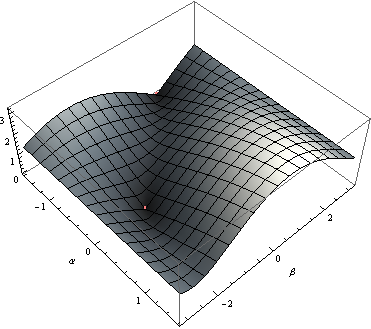
\includegraphics[width=0.8\textwidth]{figs/inversekinematics}
	\caption{Distance to $(x=1,y=1)$ over the configuration space of a two-arm manipulator. Minima corresponds to exact inverse kinematic solutions.}
	\label{fig:inversekinematics}
\end{figure}

You can now think about inverse kinematics as a path finding problem from anywhere in the configuration space to the nearest minima. A formal approach to doing this will be discussed in Section \ref{sec:advinvkinematics}. How to find shortest paths in space, that is finding the shortest route for a robot to get from A to B will be a subject of chapter \ref{chap:pathplanning}.

\section{Forward Kinematics of Mobile Robots}
Whereas the pose of a robotic manipulator is uniquely defined by its joint angles---which can be made available using encoders in almost real-time---this is not the case for a mobile robot. Here, the encoder values simply refer to wheel orientation and need to be integrated over time, which will be a huge source of uncertainty as we will later see.
What complicates matters is that for so-called \emph{non-holonomic} systems, it is not sufficient to simply measure the distance that each wheel traveled, but also when each movement was executed. 

\begin{figure}[htb!]
	\centering
		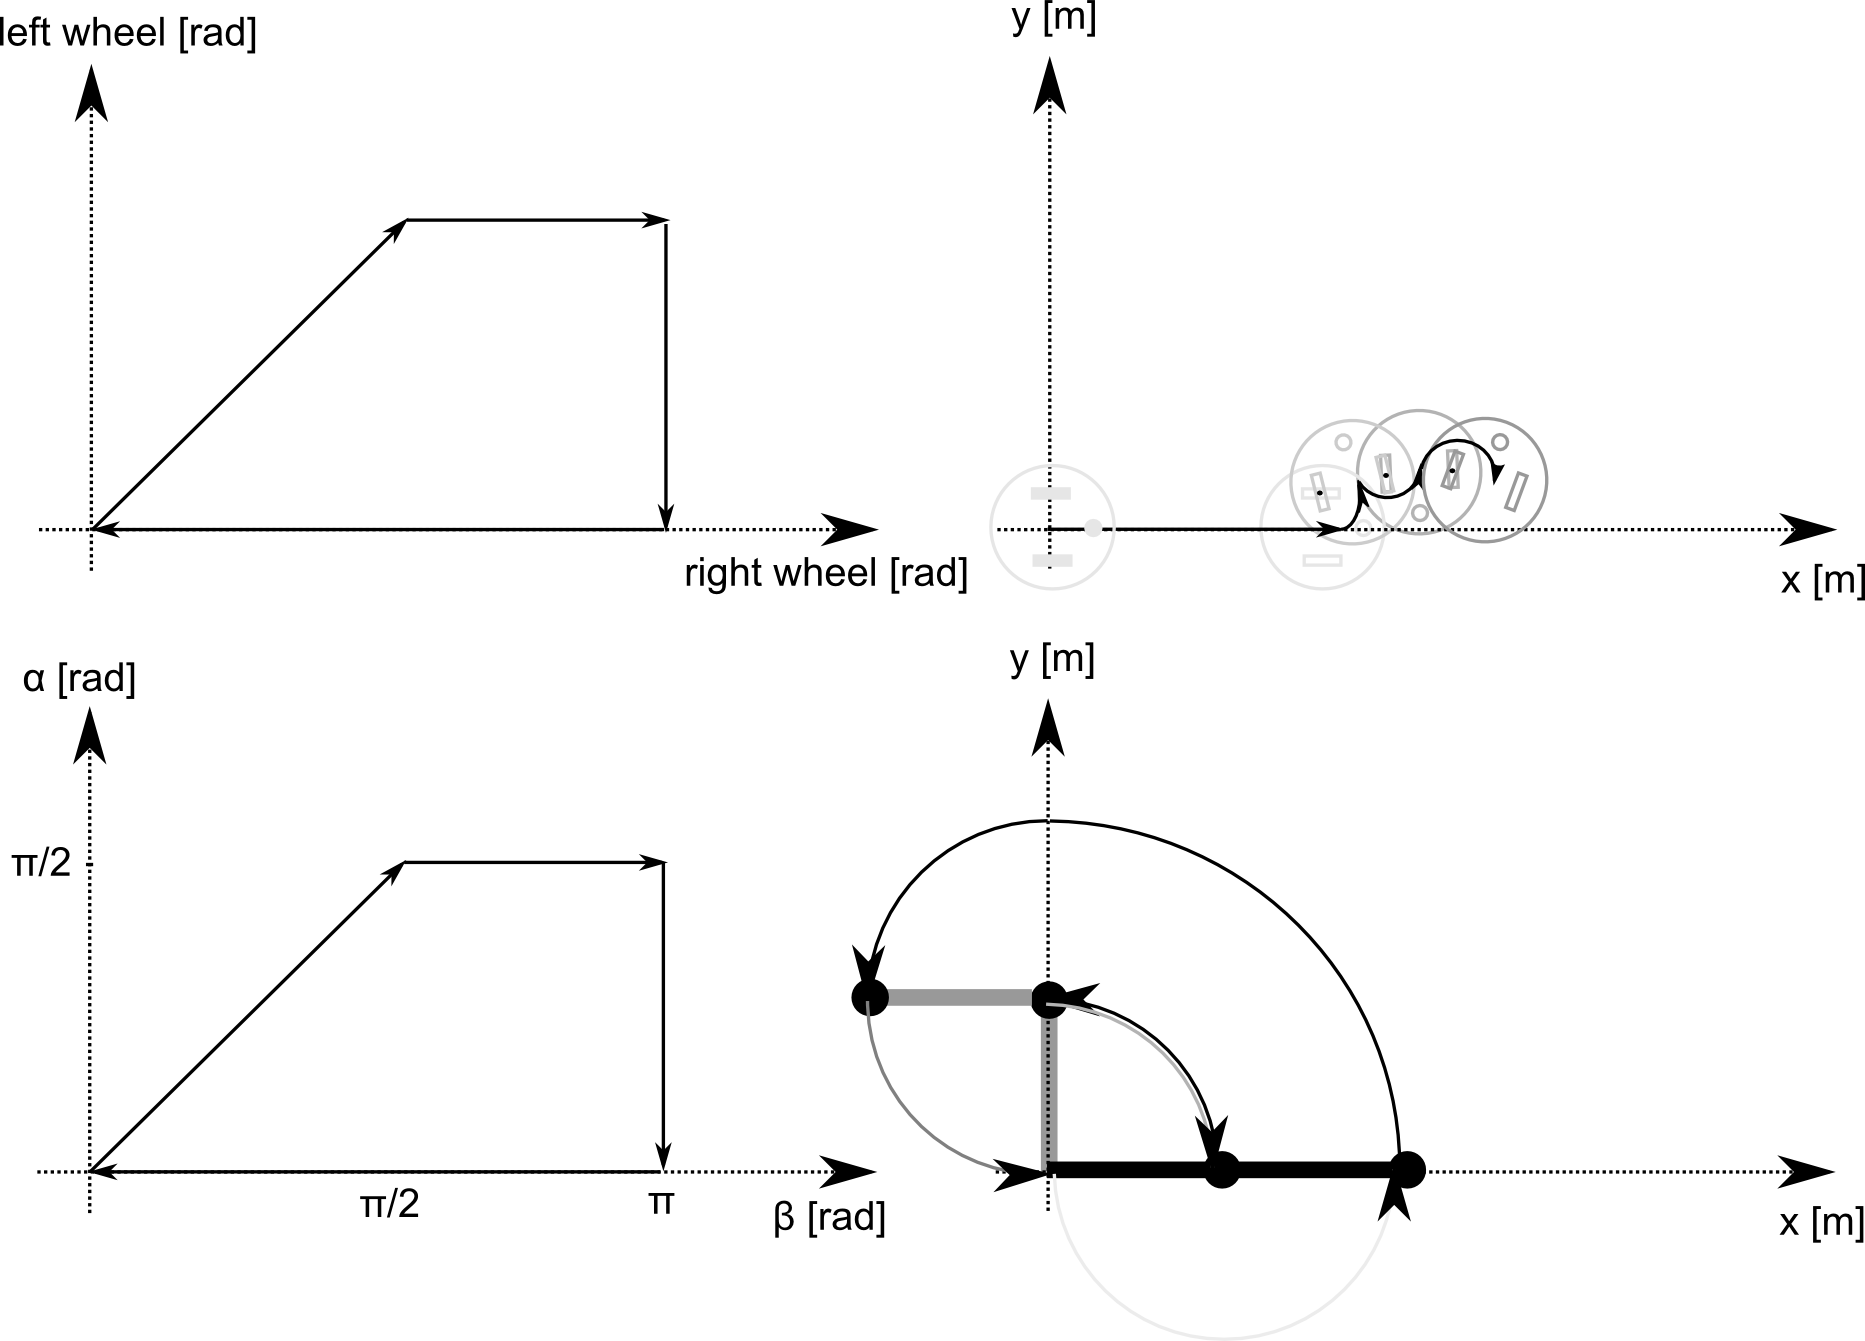
\includegraphics[width=0.95\textwidth]{figs/holonomy.png}
	\caption{Configuration space (left) and workspace (right) for a non-holonomic mobile robot (top) and a holonomic manipulator (bottom). Closed trajectories in configuration space result in closed trajectories in the workspace if the robot's kinematics is holonomic.}
	\label{fig:holonomy}
\end{figure}

A system is non-holonomic\index{Non-holonomic}\index{Holonomic} when closed trajectories in its configuration space (reminder: the configuration space of a two-link robotic arm is spanned by the possible values of each angle) may not have it return to its original state.  A simple arm is holonomic, as each joint position corresponds to a unique position in space. Going through whatever trajectory that comes back to the starting point in configuration space, will put the robot at the exact same position. A train on  a track is holonomic: moving its wheels backwards by the same amount they have been moving forward brings the train to the exact same position in space. A car and a differential-wheel robot are non-holonomic vehicles: performing a straight line and then a right-turn leads to the same amount of wheel rotation than doing a right turn first and then going in a straight line; getting the robot to its initial position requires not only to rewind both wheels by the same amount, but also getting their relative speeds right. The configuration and corresponding workspace trajectories for a non-holonomic and a holonomic robot are shown in Figure \ref{fig:holonomy}. Here, a robot first moves on a straight line (both wheels turn an equal amount). Then the left wheel remains fixed and only the right wheel turns forward. The the right wheel remain fixed and the left wheel turns backward. Finally, the right wheel turns backward, arriving at the initial encoder values (zero). Yet, the robot does not return to its origin. Performing a similar trajectory in the configuration space of a two-link manipulator instead, let the robot return to its initial position. 

It should be clear by now that for a mobile robot, not only traveled distance per wheel matters, but also the speed of each wheel as a function of time. Instead, this information was not required to uniquely determine the pose of a manipulating arm. Lets introduce the following conventions. We will establish a world coordinate system $\{I\}$, which is known as the inertial frame by convention (Figure \ref{fig:mobilerobot}). We establish a coordinate system $\{R\}$ on the robot and express the robot's speed $^R\dot{\xi}$ as a vector $ ^R\dot{\xi}=[^R\dot{x}, ^R\dot{y}, ^R\dot{\theta}]^T$. Here $^R\dot{x}$ and $^R\dot{y}$ correspond to the speed along the x and y directions in $\{R\}$, whereas $^R\dot{\theta}$ corresponds to the rotation around the imaginary z-axis, that you can imagine to be sticking out of the ground. We denote speeds with dots over the variable name, as speed is simply the derivative of distance.  Think about the robot's position in $\{R\}$ real quick. It is always zero, as the coordinate system is fixed on the robot. Therefore, velocities are the only interesting quantities in this coordinate system and we need to understand how velocities in $\{R\}$ map to positions in $ \{I\}$, which we denote by $^I\xi=[^Ix, ^Iy, ^I\theta]^T$. These coordinate systems are shown in Figure \ref{fig:mobilerobot}. 

\begin{figure}[htb!]
	\centering
		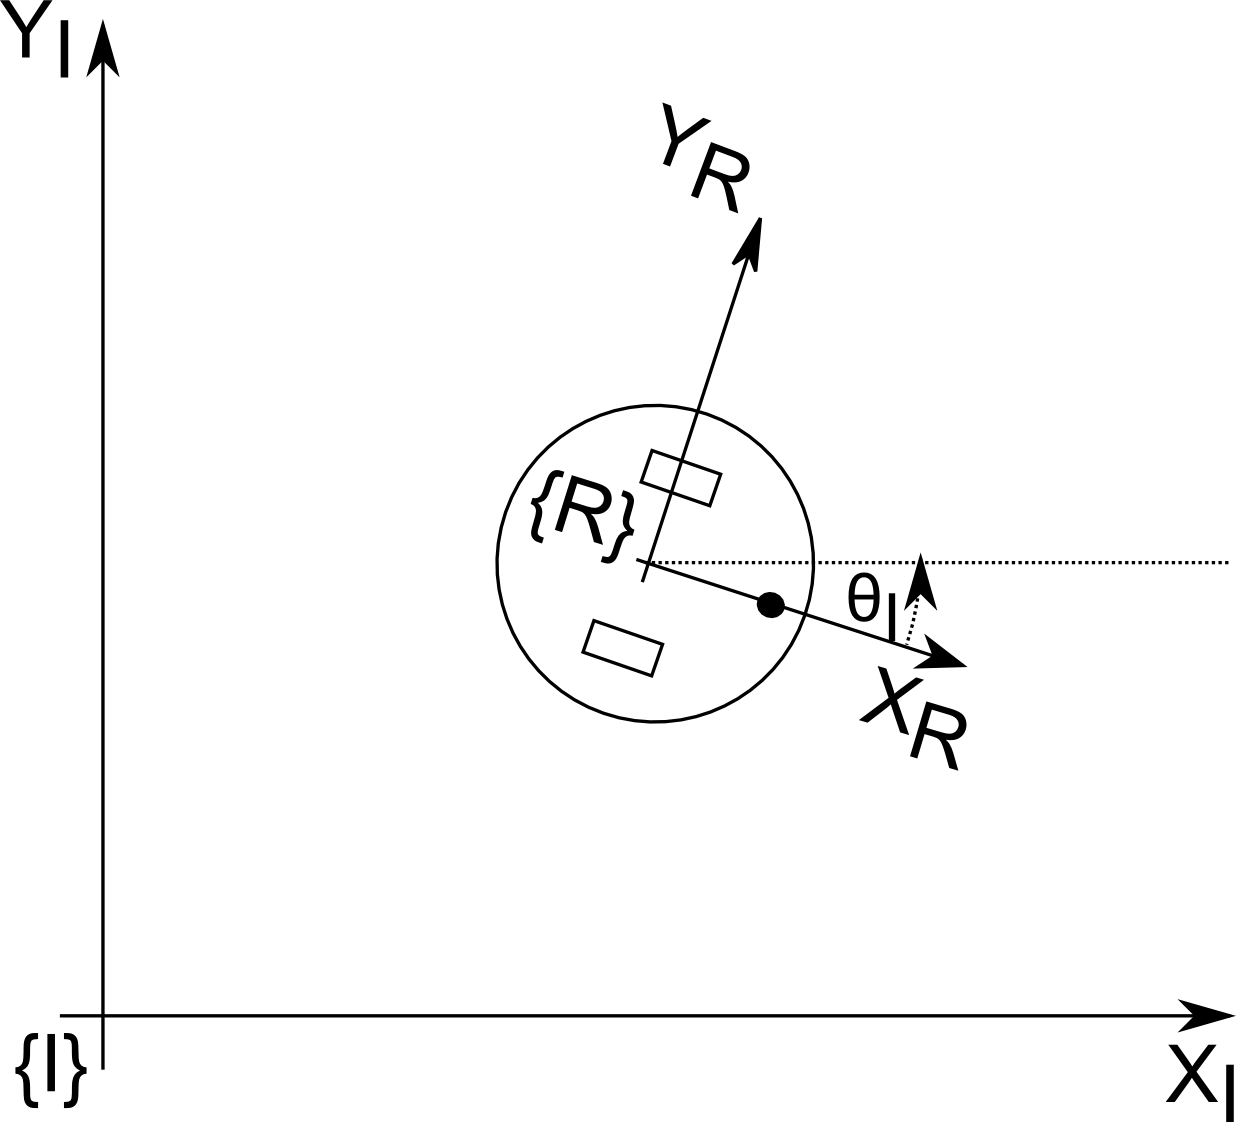
\includegraphics[width=0.85\textwidth]{figs/mobilerobot.png}
	\caption{Mobile robot with local coordinate system \{R\} and world frame \{I\}. The arrows indicate the positive direction of position and orientation vectors.}
	\label{fig:mobilerobot}
\end{figure}



Notice that the positioning of the coordinate frames and their orientation are arbitrary. Here, we chose to place the coordinate system in the center of the robot's axle and align $^Rx$ with its default driving direction.

In order to calculate the robot's position in the inertial frame, we need to first find out, how speed in the robot coordinate frame maps to speed in the inertial frame. This can be done again by employing trigonometry. There is only one complication: a movement into the robot's x-axis might lead to movement along both the x-axis and the y-axis of the world coordinate frame. By looking at the figure above, we can derive the following components to $\dot{x}_I$. First, 
\begin{equation}
\dot{x}_{I,x}=cos(\theta) \dot{x}_R.
\end{equation}

There is also a component of motion coming from $ \dot{y}_R$ (ignoring the kinematic constraints for now, see below).  For negative $ \theta$, as in Figure \ref{fig:mobilerobot}, a move along $y_R$ would let the robot move into negative $ X_I$ direction. The projection from $ \dot{y}_R$ is therefore given by 
\begin{equation}
\dot{x_{I,y}}=-sin(\theta)\dot{y_R}.
\end{equation} 
We can now write
\begin{equation}
\dot{x_I}=cos(\theta) \dot{x_R} - sin(\theta) \dot{y_R}.
\end{equation}
Similar reasoning leads to
\begin{equation}
\dot{y_I}=sin(\theta) \dot{x_R} + cos(\theta) \dot{y_R}
\end{equation}
and
\begin{equation}
\dot{\theta_I}=\dot{\theta_R}
\end{equation}
which is the case because both robot's and world coordinate system share the same z-axis in this example. We can now conveniently write
\begin{equation}
\dot{\xi_I}=^I_RT(\theta)\dot{\xi_R}
\end{equation}
with
\begin{equation}
^I_RT(\theta)=\left(\begin{array}{ccc}
cos(\theta) & -sin(\theta) & 0 \\
sin(\theta) & cos(\theta) & 0 \\
0 & 0 & 1\end{array}\right)
\end{equation}

We are now left with the problem of how to calculate the speed $ \dot{\xi_R}$ in robot coordinates. For this, we make use of the \emph{kinematic constraints}\index{Kinematic constraints} of the robotic wheels. For a standard wheel, the kinematic constraints are that every rotation of the wheel leads to strictly forward or backward motion and does not allow side-way motion or sliding. We can therefore calculate the forward speed of a wheel $ \dot{x}$ using its rotational speed $ \dot{\phi}$ (assuming the encoder value/angle is expressed as $ \phi$) and radius $ r$ by 
\begin{equation}
\dot{x}=\dot{\phi}r.
\end{equation}
This becomes apparent when considering that the circumference of a wheel with radius $ r$ is $ 2\pi r$. The distance a wheel rolls when turned by the angle $ \phi$ (in radians) is therefore $ x=\phi r$ (Figure \ref{wheelrotation}, left). Taking the derivative of this expression on both sides leads to the above expression.

\begin{figure}[htb!]
	\centering
		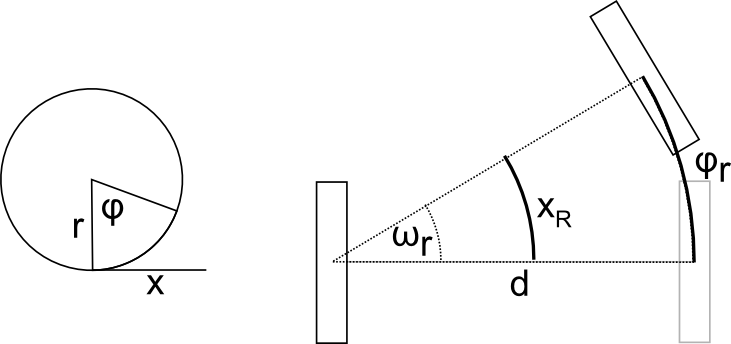
\includegraphics[width=0.9\textwidth]{figs/wheelrotation.png}
	\caption{Left: relationship between rotation and translation. Right: Differential wheel robot pivoting around its left wheel.}
	\label{fig:wheelrotation}
\end{figure}

How each of the two wheels in our example contributes to the speed of the robot's center---where its coordinate system is anchored---requires the following trick: we calculate the contribution of each individual wheel while assuming all other wheels remaining un-actuated. In this example, the distance traveled by the center point is exactly half of that traveled by each individual wheel, assuming the non-actuated wheel rotating around its ground contact point (Figure \ref{fig:wheelrotation}, right). We can therefore write
\begin{equation}
\dot{x_R}=\frac{r\dot{\phi_l}}{2}+\frac{r\dot{\phi_r}}{2}
\end{equation}
given the speeds $ \dot{\phi_l}$ and $ \dot{\phi_r}$ of the left and the right wheel, respectively.

\begin{framed}
Think about how the robot's speed along its y-axis is affected by the wheel-speed given the coordinate system in the drawing above. Think about the kinematic constraints that the standard wheels impose.
\end{framed}

Hard to believe at first, but the speed of the robot along its y-axis is always zero. This is because the constraints of the standard wheel tell us that the robot can never slide. We are now left with calculating the rotation of the robot around its z-axis. That there is such a thing can be immediately seen when imaging the robot's wheels spinning in opposite directions. We will again consider each wheel independently. Assuming the left wheel to be non-actuated, spinning the right wheel forwards will lead to counter-clockwise rotation. Given an axle diameter (distance between the robot's wheels) $ d$, we can now write
\begin{equation}
\omega_r d = \phi_r r
\end{equation}
with $ \omega_r$ the angle of rotation around the left wheel (Figure \ref{fig:wheelrotation}, right). Taking the derivative on both sides yields speeds and we can write
\begin{equation}
\dot{\omega_r} = \frac{\dot{\phi_r} r}{d}
\end{equation}
Adding the rotation speeds up (with the one around the right wheel being negative based on the right-hand grip rule), leads to

\begin{equation}
\dot{\theta}=\frac{\dot{\phi_r} r}{d}-\frac{\dot{\phi_l} r}{d}
\end{equation}

Putting it all together, we can write

\begin{equation}
\left(\begin{array}{c} \dot{x_I}\\\dot{y_I}\\\dot{\theta}\end{array}\right)=\left(\begin{array}{ccc}
cos(\theta) & -sin(\theta) & 0 \\
sin(\theta) & cos(\theta) & 0 \\
0 & 0 & 1\end{array}\right)\left(\begin{array}{c}\frac{r\dot{\phi_l}}{2}+\frac{r\dot{\phi_r}}{2}\\0\\\frac{\dot{\phi_r} r}{d}-\frac{\dot{\phi_l} r}{d}\end{array}\right)
\end{equation}

\section{Inverse Kinematics of Mobile Robots}
The main problem for the engineer is now to find out how to chose the control parameters to reach a desired position. This problem is known as inverse kinematics. Solving the inverse kinematics in closed form is not always possible, however. It can be done for the differential wheel platform we studied above. Lets first establish how to calculate the necessary speed of the robot's center given a desired speed $ \dot{\xi_I}$ in world coordinates. We can transform the expression $ \dot{\xi_I}=T(\theta)\dot{\xi_R}$ by multiplying both sides with the inverse of $ T(\theta)$:

\begin{equation}
T^{-1}(\theta)\dot{\xi_I}=T^{-1}(\theta)T(\theta)\dot{\xi_R}
\end{equation}
which leads to $ \dot{\xi_R}=T^{-1}(\theta)\dot{\xi_I}$. Here

\begin{equation}
T^{-1}=\left(\begin{array}{ccc}cos \theta & sin \theta & 0 \\ -sin \theta & cos \theta & 0 \\ 0 & 0 & 1\end{array}\right)
\end{equation}

which can be determined by actually performing the matrix inversion or by deriving the trigonometric relationships from the drawing.  Similarly, we can now solve

\begin{equation}
\left(\begin{array}{c} \dot{x_R}\\\dot{y_R}\\\dot{\theta}\end{array}\right)=\left(\begin{array}{c}\frac{r\dot{\phi_l}}{2}+\frac{r\dot{\phi_r}}{2}\\0\\\frac{\dot{\phi_r} r}{d}-\frac{\dot{\phi_l} r}{d}\end{array}\right)
\end{equation}

for $ \phi_l$, $ \phi_r$. (do this!) You will now see that your kinematic constraints actually render some desired velocities, namely those that would lead to non-negative $ \dot{y_R}$ unfeasible.


\section{Car-like steering}
Differential wheel drives are very popular in mobile robotics as they are very easy to build, maintain, and control. Although not holonomic, a differential drive can approximate the function of a fully holonomic robot by first driving on the spot to achieve the desired heading and then driving straight. Drawbacks of the differential drive are its reliance on a caster wheel, which performs poorly at high speeds , and difficulties in driving straight lines as this requires both motors to drive at the exact same speed.


These drawbacks are mitigated by car-like mechanisms, which are driven by a single motor and can steer their front wheels. This mechanism is known as ``Ackermann steering'' \index{Ackermann steering} and illustrated to the right. Ackermann steering should not be confused with ``turntable'' steering \index{Turntable steering} where the front wheels are fixed on an axis with central pivot point. Instead, each wheel has its own pivot point and the system is constrained in such a way that all wheels of the car drive on circles with a common center point, avoiding skid.

\subsection{Forward Kinematics of Ackermann Steering}
As the Ackermann mechanism lets all wheels drive on circles with a common center point, its kinematics can be approximated by those of a tricycle with rear-wheel drive.

Let the car have the shape of a box with length $ L$ between rear and front axis. Let the center point of the common circle described by all wheels be distance $ R$ from the car's longitudinal center line.  Then, the steering angle $ \phi$ is given by

\begin{equation}
\tan \phi = \frac{L}{R}
\end{equation}


\subsection{Coordinate frames for a simplified car-like steering}
Let the robot coordinate system $ (x_r,y_r,\theta_r)$ be centered on the car's rear axis. Then, $ \dot{x}_r$ is the car's speed given by the speed of the car's engine. We can now derive expressions for the car's position in world coordinates $ (x_w,y_w,\theta_w)$.  (Remember: as the car is non-holonomic we can derive the kinematics only for speeds, the derivative of position, without integrating.)

\begin{eqnarray}
\dot{x}_w&=&\cos{\theta_w}\dot{x}_r\\
\dot{y}_w&=&\sin{\theta_w}\dot{x}_r\\
\dot{\theta}_w&=&\frac{\tan{\phi}}{L}\dot{x}_r
\end{eqnarray}

The last expression directly follows from the rule that the tangent of an angle is equivalent to the ratio of its opposite to adjacent edges. At this point it is worth recalling that $ \dot{y}_r=0$, no matter what, as a simple model does not allow the robot to skid. Therefore, the steering angle $ \phi$ only affects the rotation of the car.

At this point, you have expressions for predicting the movement of the car's bounding box through space as a function of speed and steering angle. The angles of the left and the right wheel, $ \phi_l$ and $ \phi_r$ can be calculated using the fact that all wheels of the car rotate around circles with a common center point. With the distance between the two front wheels $ l$, we can therefore write

Angles of individual wheels for perfect Ackermann steering
\begin{eqnarray}
\frac{L}{R-l/2}&=\tan{(\pi/2-\phi_r)}\\
\frac{L}{R+l/2}&=\tan{(\pi/2-\phi_l)}
\end{eqnarray}
with $ R=L\tan{\phi}$, again following the rule tangent = opposite / adjacent. This is important to calculate the resulting wheel angles and to test whether they are within the constraints of the actual vehicle.


\section*{Take-home lessons}

\begin{itemize}
\item Forward kinematics are equivalent to finding a coordinate transform from a world coordinate system into a coordinate system on the robot. Such a transform is a combination of a (3x1) translation vector and a (3x3) rotation matrix that consists of the unit vectors of the robot coordinate system. Both translation and rotation can be combined into a 4x4 homogeneous transform matrix.
\item Forward and Inverse Kinematics of a mobile robot are performed with respect to the speed of the robot and not its position.
\item For calculating the effect of each wheel on the speed of the robot, you need to consider the contribution of each wheel independently.
\item Calculating the inverse kinematics analytically becomes quickly infeasible. You can then plan in configuration space of the robot using path-planning techniques.
\item The inverse kinematics of a robot involves solving the equations for the forward kinematics for the joint angles. This process is often cumbersome if not impossible for complicated mechanisms.
\item A simple numerical solution is provided by taking all partial derivatives of the forward kinematics in order to get an easily invertible expression that relates joint speeds to end-effector speeds.
The inverse kinematics problem can then be formulated as feedback control problem, which will move the end-effector towards its desired pose using small steps. Problems with this approach are local minima and singularities of the mechanism, that might render this solution infeasible.
\end{itemize}

\section*{Exercises}\small
\subsection*{Coordinate systems}
\begin{enumerate}
\item 
\begin{enumerate}
 \item Write out the entries of a rotation matrix $^A_BR$ assuming basis vectors $X_A$, $Y_A$, $Z_A$, and $X_B$, $Y_B$, $Z_B$. 
 \item Write out the entries of rotation matrix $^B_AR$.
 \end{enumerate} 
\item Assume two coordinate systems that are co-located in the same origin, but rotated around the z-axis by the angle $\alpha$. Derive the rotation matrix from one coordinate system into the other and verify that each entry of this matrix is indeed the scalar product of each basis vector of one coordinate system with every other basis vector in the second coordinate system.  
\item Consider two coordinate systems $\{B\}$ and $\{C\}$, whose orientation is given by the rotation matrix $^C_BR$ and have distance $^BP$. Provide the homogenous transform $^C_BT$ and its inverse $^B_CT$. 
\item Consider the frame $\{B\}$ that is defined with respect to frame $\{A\}$ as $\{B\}=\{^A_BR, ^AP\}$. Provide a homogeneous transfrom from $\{A\}$ to $\{B\}$.
\end{enumerate}

\subsection*{Forward and inverse kinematics}
\begin{enumerate}
\item Consider a differential wheel robot with a broken motor, i.e., one of the wheels cannot be actuated anymore. Derive the forward kinematics of this platform. Assume the right motor is broken.
\item The forward kinematics of a differential-wheel platform are given by 
\begin{equation}
\nonumber
\left(\begin{array}{c}
\dot{x}_r\\
\dot{y}_r\\
\dot{\theta}
\end{array}\right)
=
\left(\begin{array}{c}
\frac{r\dot{\phi}_l}{2}+\frac{r\dot{\phi_r}}{2}\\
0\\
\frac{r\dot{\phi}_r}{d}-\frac{r\dot{\phi_l}}{d}
\end{array}\right)
\end{equation}
Derive an expression for $\dot{\phi}_l$ and $\dot{\phi}_r$ as a function of the desired speeds $\dot{x}_r$ and $\dot{y}_r$. 
\item Consider a tri-cycle with two independent standard wheels in the rear and the stearable, driven front-wheel. Chose a suitable coordinate system and use $\phi$ as the steering wheel angle and wheel-speed $\dot{\omega}$. Provide forward and inverse kinematics. 
\end{enumerate}
\normalsize
\chapter{Path Planning}\label{chap:pathplanning}
Path-planning is an important primitive for autonomous mobile robots that lets robots find the shortest---or otherwise optimal---path between two points. Optimal paths could be paths that minimize the amount of turning, the amount of braking or whatever a specific application requires. Algorithms to find a shortest path are important not only in robotics, but also in network routing, video games and understanding protein folding.

Path-planning requires a map of the environment and the robot to be aware of its location with respect to the map. We will assume for now that the robot is able to localize itself,  is equipped with a map, and capable of avoiding temporary obstacles on its way. How to create a map, how to localize a robot, and how to deal with uncertain position information will be major foci of the reminder of this  book. The goals of this chapter are to

\begin{itemize}
\item introduce suitable map representations,
\item explain basic path-planning algorithms  ranging from Dijkstra, to A*, D* and RRT,
\item introduce variations of the path-planning problem, such as coverage path planning.
\end{itemize}

\section{Map representations}\label{sec:maps}
In order to plan a path, we somehow need to represent the environment in the computer. We differentiate between two complementary approaches: discrete and continuous approximations. In a discrete approximation, a map is sub-divided into chunks of equal (e.g., a grid or hexagonal map) or differing sizes (e.g., rooms in a building). The latter maps are also known as \emph{topological maps}.\index{Topological map} Discrete maps lend themselves well to a graph representation. Here, every chunk of the map corresponds to a vertex (also known as ``node''), which are connected by edges, if a robot can navigate from one vertex to the other. For example a road-map is a topological map, with intersections as vertices and roads as edges, labeled with their length (Figure \ref{fig:pathproblem}). Computationally, a graph might be stored as an adjacency or incidence list/matrix. A continuous approximation requires the definition of inner (obstacles) and outer boundaries, typically in the form of a polygon, whereas paths can be encoded as sequences of points defined by real numbers. Despite the memory advantages of a continuous representation, discrete maps are the dominant representation in robotics.

For mapping obstacles, the most common map is the \emph{occupancy grid} map\index{Occupancy grid}. In a grid map, the environment is discretized into squares of arbitrary resolution, e.g. 1cm x 1cm, on which obstacles are marked. In a probabilistic occupancy grid, grid cells can also be marked with the probability that they contain an obstacle. This is particularly important when the position of the robot that senses an obstacle is uncertain. Disadvantages of grid maps are their large memory requirements as well as computational time to traverse data structures with large numbers of vertices. A solution to this is storing the grid map as \emph{k-d tree}.\index{k-d tree (data structure)} A k-d tree recursively breaks the environment into $k$ pieces. For $k=4$, an area is broken into four pieces. Each of these pieces is again broken into four pieces and so on, until the desired resolution is reached. These pieces can easily be stored in a graph with each vertex having four children, which are the four pieces the vertex is broken into, or is a leaf of the tree. What makes this data structure attractive is that not all vertices need to be broken down to the smallest possible resolution. Instead only areas, which contain obstacles need to be further broken down. A grid map containing obstacles and the corresponding k-d tree, here a quadtree, are shown in Figure \ref{fig:gridvskdtree}. There is no silver bullet, and each application might require a different solution that could be a combination of different map types.

\begin{figure}
\centering
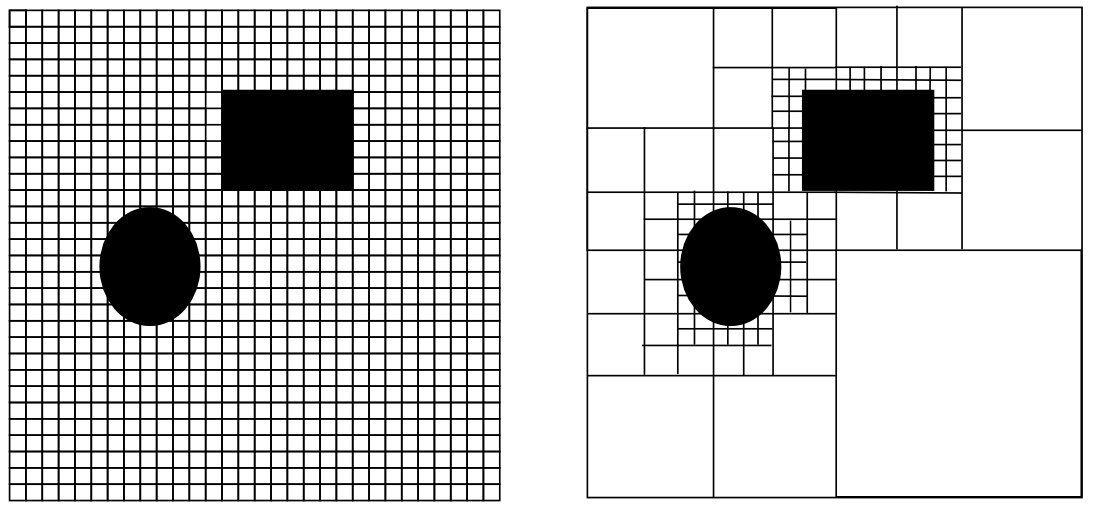
\includegraphics[width=\textwidth]{figs/gridvskdtree.png}
\caption{A grid map and its corresponding quadtree (k-d tree).\label{fig:gridvskdtree}}
\end{figure}


There exist also every possible combination of discrete and continuous representation. For example, roadmaps for GPS systems are stored as topological maps that store the GPS coordinates of every vertex, but might also contain overlays of aerial and street photography or even 3D point clouds stored in a 8-d tree, also known as a \emph{Octree}\index{Octree}. These different maps are then used at different stages of the path planning stage. 


\section{Path-Planning Algorithms}
The problem to find a ``shortest'' path from one vertex to another through a connected graph is of interest in multiple domains, most prominently in the internet, where it is used to find an optimal route for a data packet. The term ``shortest'' refers here to the minimum cumulative edge cost, which could be physical distance (in a robotic application), delay (in a networking application) or any other metric that is important for a specific application. An example graph with arbitrary edge-lengths is shown in Figure \ref{fig:pathproblem}. 

\begin{figure}[!htb]
\centering
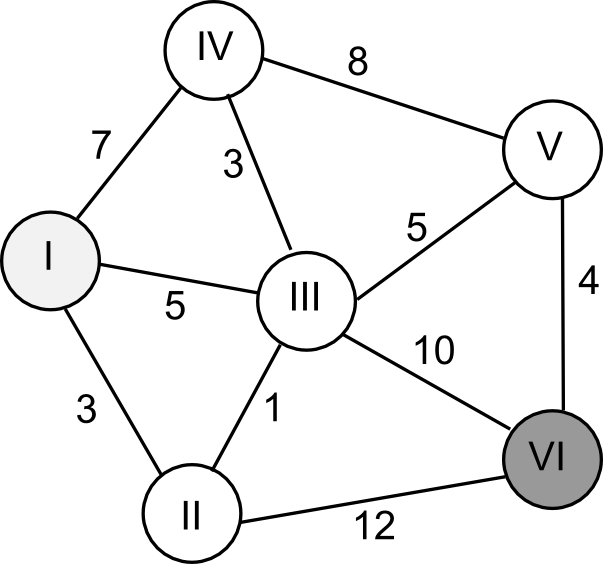
\includegraphics[width=0.6\textwidth]{figs/dijkstra}
\caption{A generic path planning problem from vertex I to vertex VI. The shortest path is I-II-III-V-VI with length 13. \label{fig:pathproblem}}
\end{figure}

\subsection{Robot embodiment}
In order to deal with the physical embodiment of the robot, which complicates the path-planning process, the robot is reduced to a point-mass and all the obstacles in the environment are grown by half of the longest extension of the robot from its center. This representation is known as configuration space \index{Configuration space}as it reduces the representation of the robot to its $x$ and $y$ coordinates in the plane. An example is shown in Figure \ref{fig:cspace}. The configuration space can now either be used as a basis for a grid map or a continuous representation. 

\begin{figure}[!htb]
\centering
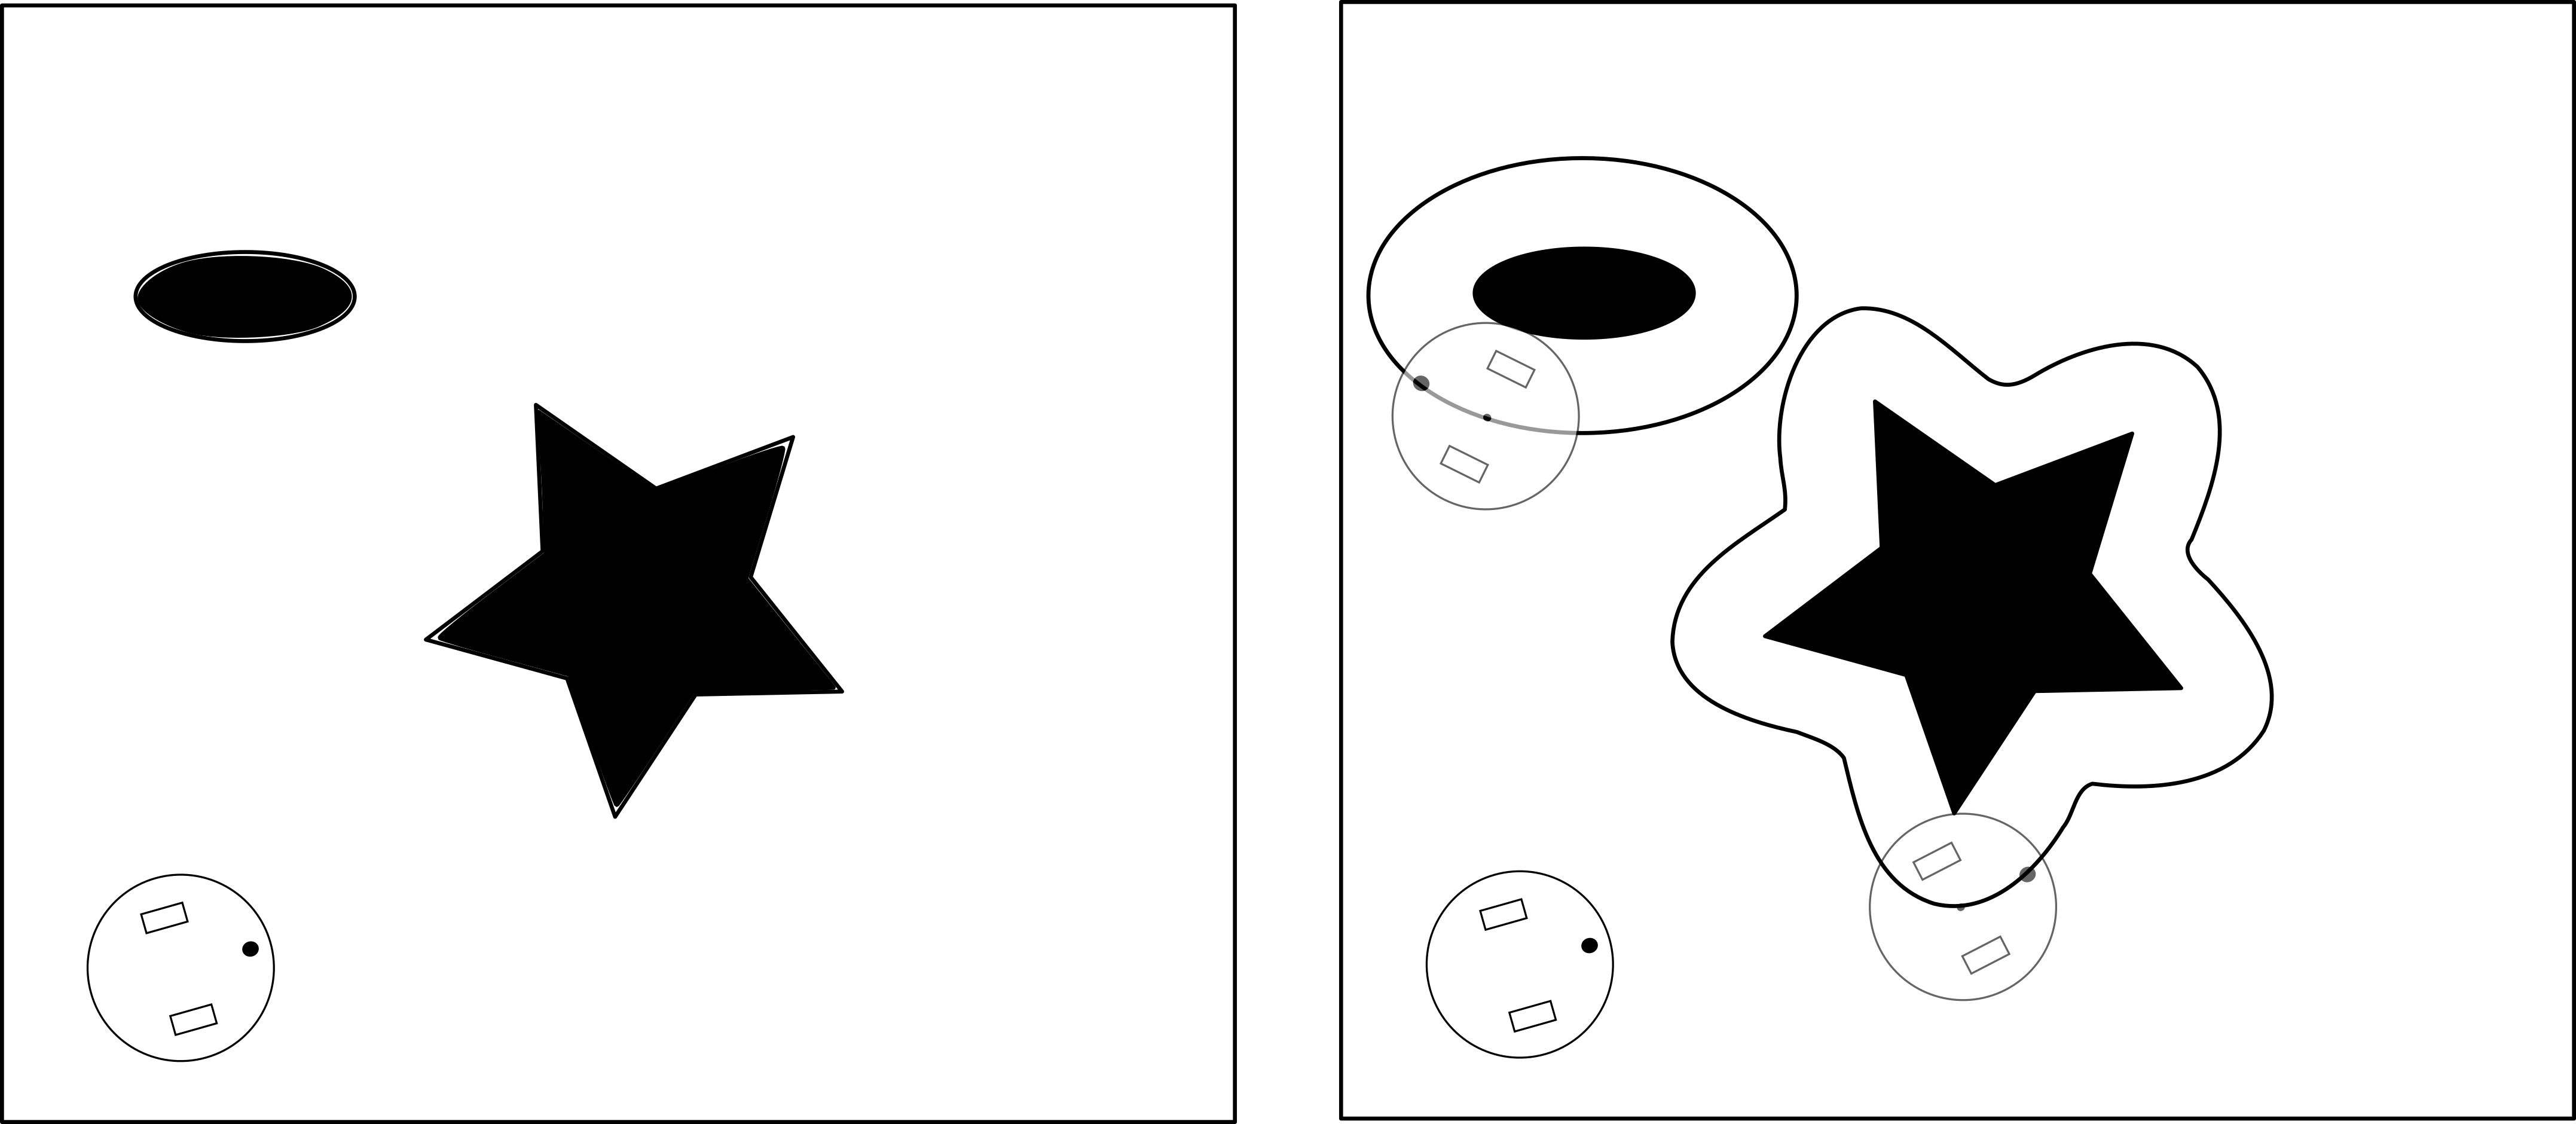
\includegraphics[width=0.9\textwidth]{figs/configurationspace}
\caption{A map with obstacles and its representation in configuration space, which can be obtained by growing each obstacle by the robot's extension. \label{fig:cspace}}
\end{figure}


\subsection{Dijkstra's algorithm}\index{Dijkstra's Shortest Path Algorithm}
One of the earliest and simplest algorithms is Dijkstra's algorithm \cite{dijkstra1959note}. Starting from the initial vertex where the path should start, the algorithm marks all direct neighbors of the initial vertex with the cost to get there. It then proceeds from the vertex with the lowest cost to all of its adjacent vertices and marks them with the cost to get to them via itself if this cost is lower. Once all neighbors of a vertex have been checked, the algorithm proceeds to the vertex with the next lowest cost. Once the algorithm reaches the goal vertex, it terminates and the robot can follow the edges pointing towards the lowest edge cost.

In Figure \ref{fig:pathproblem}, Dijkstra would first mark nodes II, III and IV with cost 3, 5 and 7 respectively. It would then continue to explore all edges of node II, which so far has the lowest cost. This would lead to the discovery that node III can actually be reached in $3+1<5$ steps, and node III would be relabeled with cost 4. In order to completely evaluate node II, Dijkstra needs to evaluate the remaining edge before moving on and label node VI with $3+12=15$.

The node with the lowest cost is now node III (4). We can now relabel node VI with 14, which is smaller than 15, and label node V with $4+5=9$, whereas node IV remains at $4+3=7$. Although we have already found two paths to the goal, one of which better than the other, we cannot stop as there still exist nodes with unexplored edges and overall cost lower than 14. Indeed, continuing to explore from node V leads to a shortest path I-II-III-V-VI of cost 13, with no remaining nodes to explore.

As Dijkstra would not stop until there is no node with lower cost than the current cost to the goal, we can be sure that a shortest path will be found if it exists. We can say that the algorithm is \emph{complete}.\index{Complete (algorithm)}

As Dijkstra will always explore nodes with the least overall cost first, the environment is explored comparably to a wave front originating from the start vertex, eventually arriving at the goal. This is of course highly inefficient in particular if Dijkstra is exploring nodes away from the goal. This can be visualized by adding a couple of nodes to the left of node I in Figure \ref{fig:pathproblem}. Dijkstra will explore all of these nodes until their cost exceeds the lowest found for the goal. This can also be seen when observing Dijkstra's algorithm on a grid, as shown in Figure \ref{fig:dijkstragrid}. 

\begin{figure}[htb]
\centering
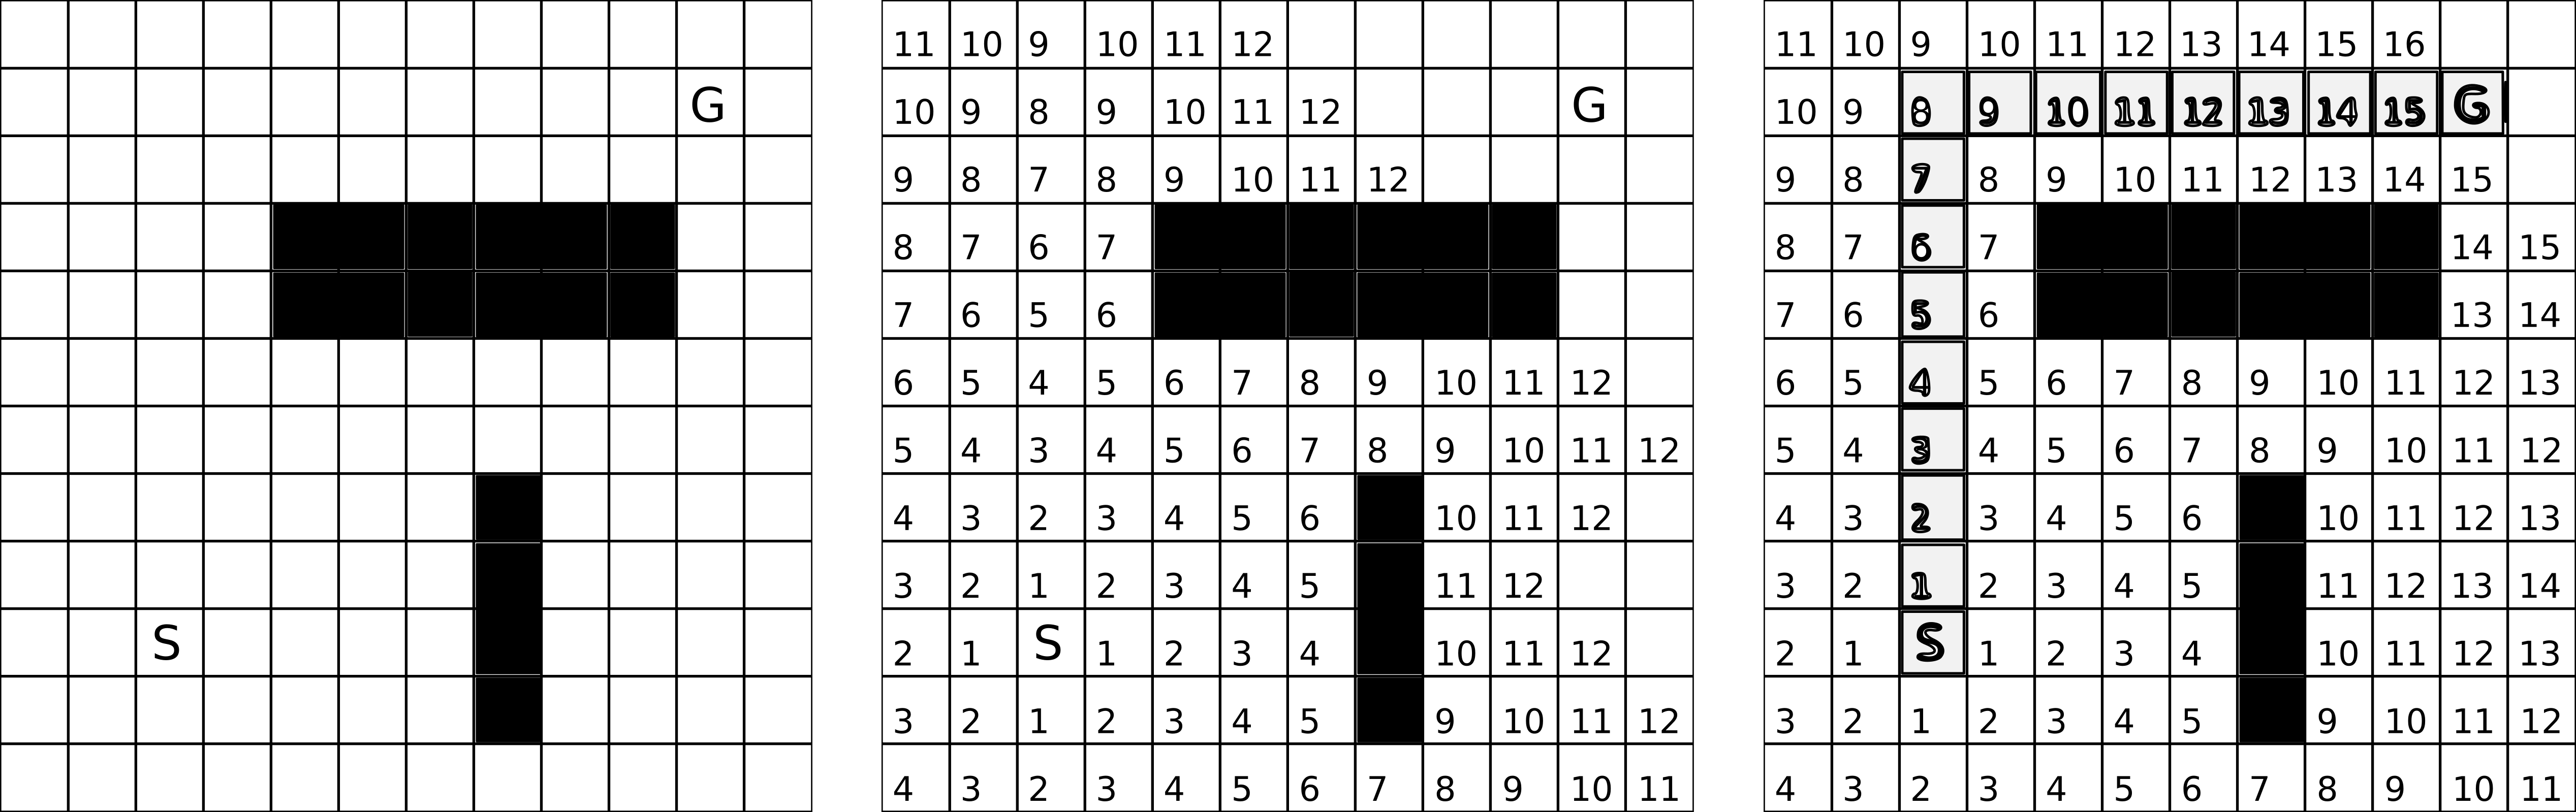
\includegraphics[width=0.9\textwidth]{figs/dijkstragrid}
\caption{Dijkstra's algorithm finding a shortest path from `S' to 'G' assuming the robot can only travel laterally (not diagonally) with cost one per grid cell. Note the few number of cells that remain unexplored once the shortest path (grey) is found, as Dijkstra would always consider a cell with the lowest path cost first.\label{fig:dijkstragrid}}
\end{figure}

\subsection{A*}\label{sec:astar}\index{A* Shortest Path Algorithm}
Instead of exploring in all directions, knowledge of an approximate direction of the goal could help avoiding exploring nodes that are obviously wrong to a human observer. Such special knowledge that such an observer has can be encoded using a \emph{heuristic function}\index{Heuristic function}, a fancier word for a ``rule of thumb''. For example, we could give priority to nodes that have a lower estimated distance to the goal than others. For this, we would mark every node not only with the actual distance that it took us to get there (as in Dijkstra's algorithm), but also with the estimated cost ``as the crows flies'', for example by calculating the Euclidean distance or the \emph{Manhattan distance}\index{Manhattan distance} between the vertex we are looking at and the goal vertex. This algorithm is known as A* \cite{hart1968formal}. Depending on the environment, A* might accomplish search much faster than Dijkstra's algorithm, and performs the same in the worst case. This is illustrated in Figure \ref{fig:astargrid} using the Manhattan distance metric, which does not allow for diagonal movements. 

\begin{figure}[htb]
\centering
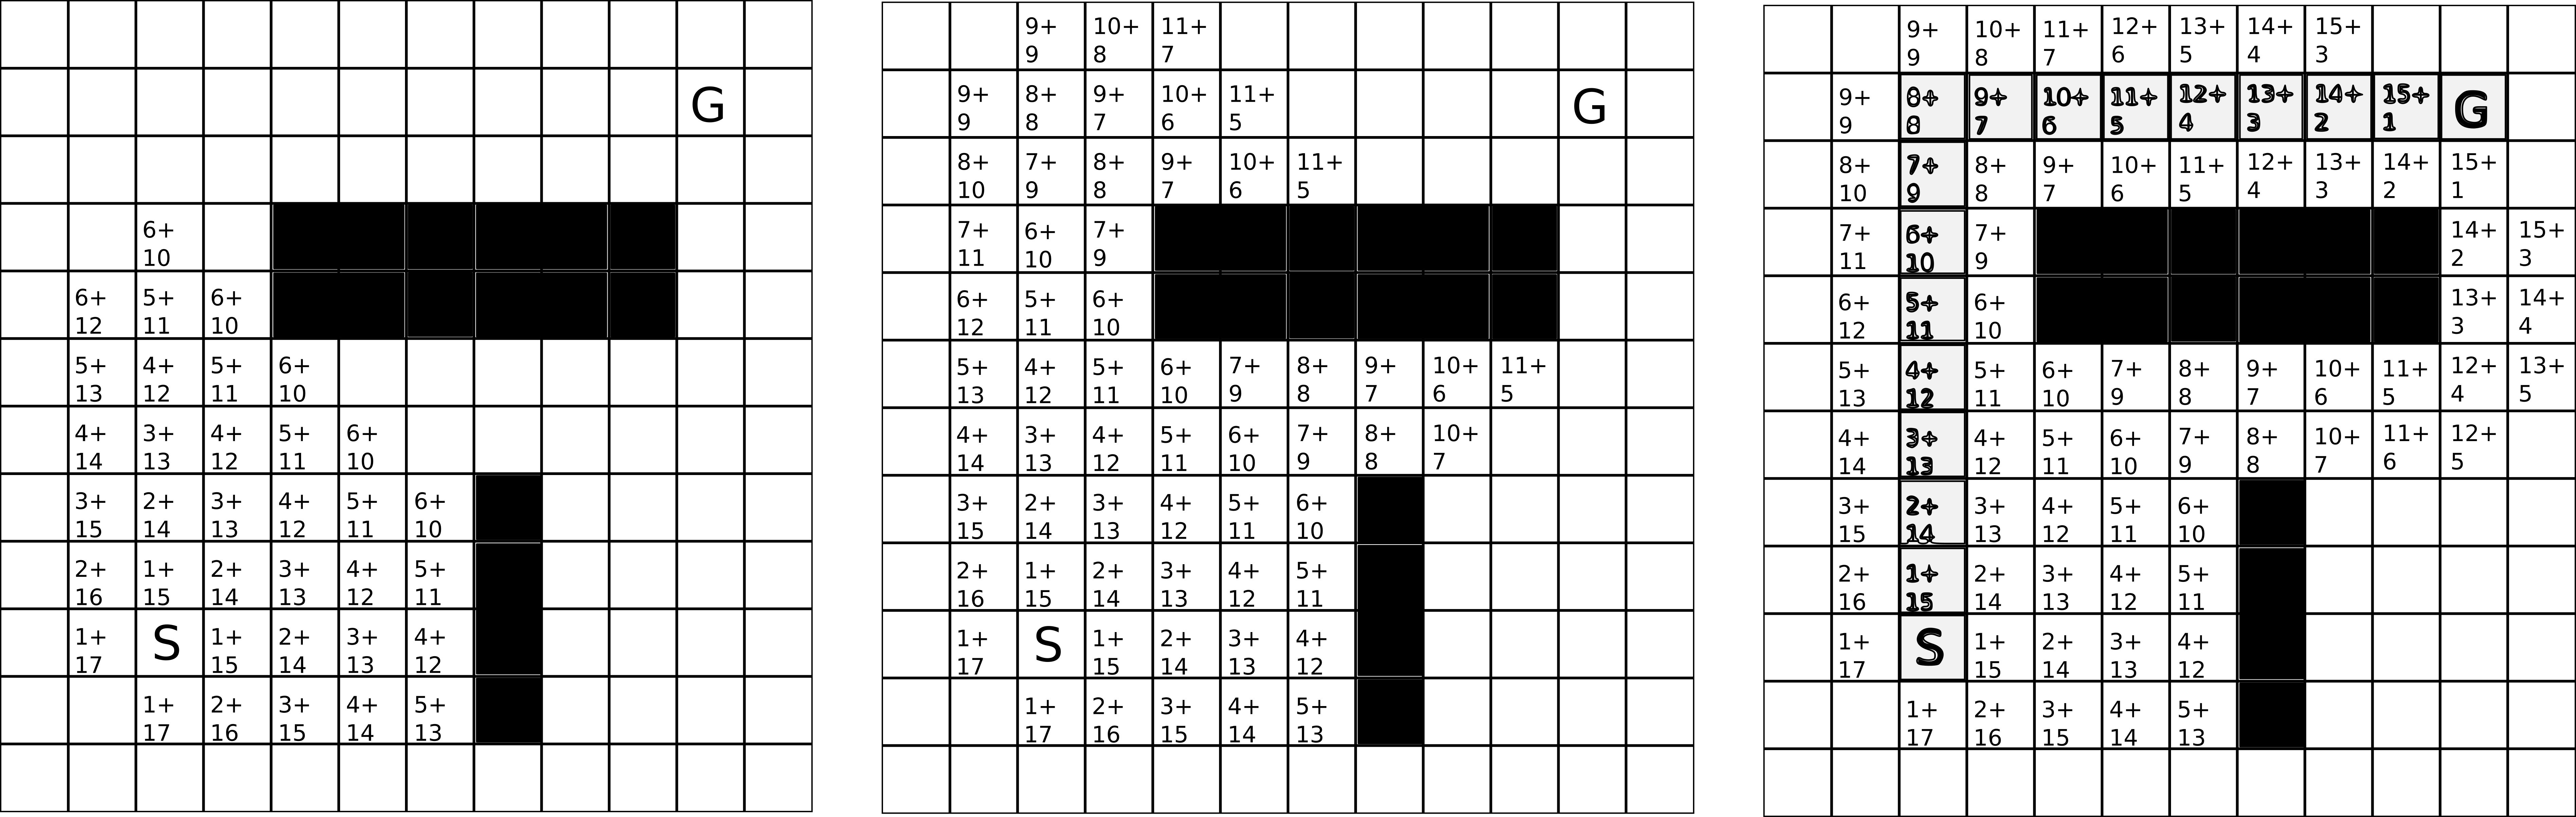
\includegraphics[width=0.9\textwidth]{figs/astargrid}
\caption{Finding a shortest path from `S' to 'G' assuming the robot can only travel laterally (not diagonally) with cost one per grid cell using the A* algorithm. Much like Dijkstra, A* evaluates only the cell with the lowest cost, but takes an estimate of the remaining distance into account.\label{fig:dijkstragrid}}
\end{figure}

An extension of A* that addresses the problem of expensive re-planning when obstacles appear in the path of the robot, is known as D* \cite{stentz1994optimal}. Unlike A*, D* starts from the goal vertex and has the ability to change the costs of parts of the path that include an obstacle. This allows D* to re-plan around an obstacle while maintaining most of the already calculated path.\index{D*}

A* and D* become computationally expensive when either the search space is large, e.g., due to a fine-grain resolution required for the task, or the dimensions of the search problem are high, e.g. when planning for an arm with multiple degrees of freedom. Solutions to these problems are provided by sampling-based path planning algorithms that are described further below.




\section{Sampling-based Path Planning}
The previous sections have introduced a series of complete algorithms for the path planning problem, i.e. they will find a solution eventually if it exists. Complete solutions are often unfeasible, however, when the possible state space is large. This is the case for robots with multiple degrees of freedom such as arms. In practice, most algorithms are only \emph{resolution complete}\index{Resolution complete}, i.e., only complete if the resolution is fine-grained enough, as the state-space needs to be somewhat discretized for them to operate (e.g., into a grid) and some solutions might be missed as a function of the resolution of the discretization.

Instead of evaluating all possible solutions or using a non-complete Jacobian-based inverse kinematic solution, sampling-based planners create possible paths by randomly adding points to a tree until some solution is found or time expires. As the probability to find a path approaches one when time goes to infinity, sampling-based path planners are \emph{probabilistic complete}\index{Probabilistic complete}. Prominent examples of sampling-based planners are \emph{Rapidly-exploring Random Trees} (RRT)\index{Rapidly-exploring Random Tree}\index{RRT}\cite{lavalle1998rapidly} and \emph{Probabilistic Roadmaps}\index{Probabilistic Roadmaps}\index{PRM}(PRM) \cite{kavraki1996probabilistic}. An example execution of RRT for an unknown goal, thereby reducing the path-planning problem to a search problem is shown in Figure \ref{fig:rrt}.

\begin{figure}
\centering
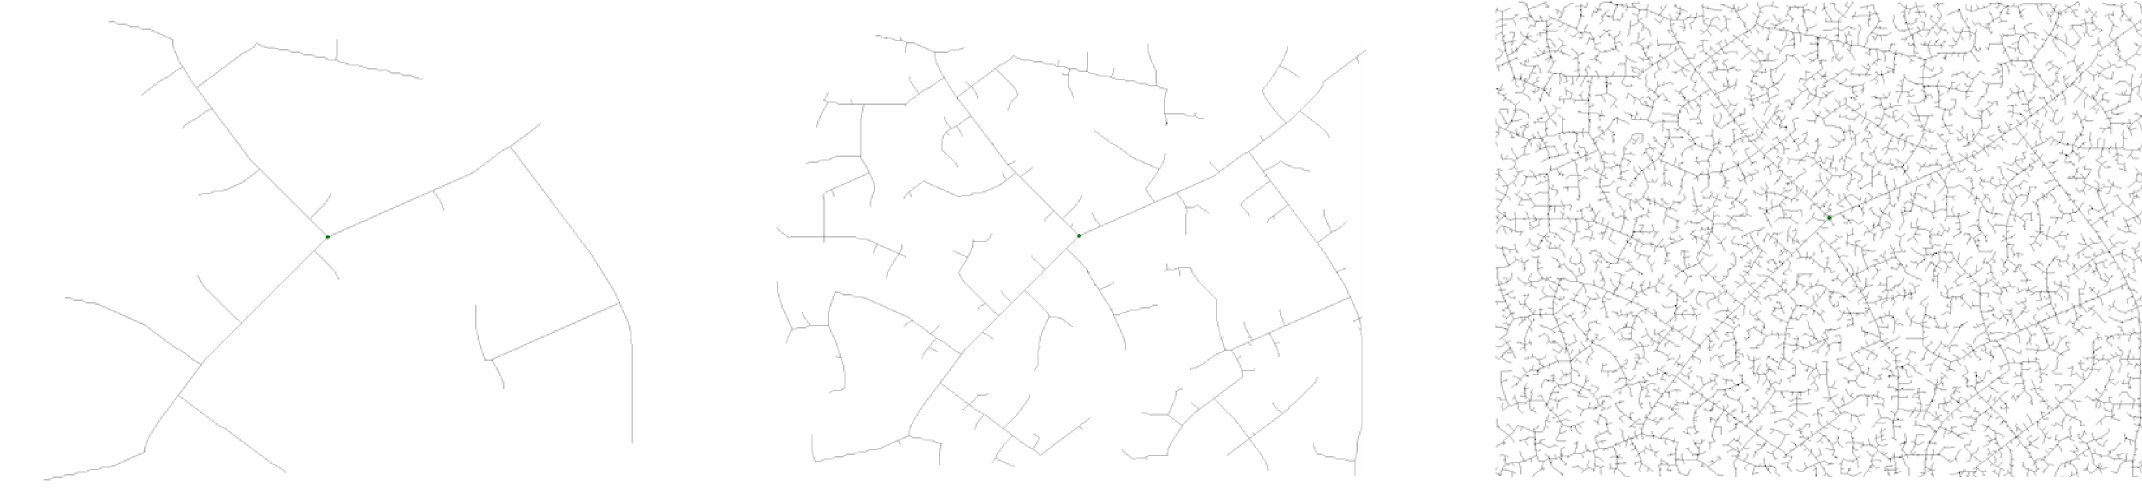
\includegraphics[width=\textwidth]{figs/rrt}
\caption{Random exploration of a 2D search space by randomly sampling points and connecting them to the graph.\label{fig:rrt}}
\end{figure}

This example illustrates well how a sampling-based planner can quickly explore a large portion of space and refines a solution as time goes on. Whereas RRT can be understood as growing a single tree from a robot's starting point until one of its branches hit a goal, probabilistic road-maps create a tree by randomly sampling points in the state-space, testing whether they are collision-free, connecting them with neighboring points using paths that reflect the kinematics of a robot, and then using classical graph shortest path algorithms to find shortest paths on the resulting structure. The advantage of this approach is clearly that such a probabilistic roadmap has to be created only once (assuming the environment is not changing) and can then be used for multiple queries. PRMs are therefore a \emph{multi-query} path-planning algorithm.\index{Multi-query (path-planning)} In contrast, RRT's are known as \emph{single-query}\index{Single-query (path-planning)} path-planning algorithms.

In practice, the boundary between the different historic algorithms has become very diffuse, and single-query and multi-query variants of both RRT and PRM exist. It is important to note that there is no silver bullet algorithm/heuristic and even their parameter-sets are highly problem-specific. We will therefore limit our discussion on useful heuristics that are common to sampling-based planners.

\subsection{Basic Algorithm}
Let $ \mathcal{X}$ be a $ d$-dimensional state-space. This can either be the robot's state given in terms of translation and rotations (6 dimensions), a subset thereof, or the joint space with one dimension per possible joint angle. Let $ \mathcal{G} \subset \mathcal{X}$ be a  d-ball (d-dimensional sphere) in the state-space that is considered to be the goal, and $ t$ the allowed time. A tree planner proceeds as follows:

\begin{verbatim}
Tree=Init(X,start);
WHILE ElapsedTime() < t AND NoGoalFound(G) DO
 newpoint = StateToExpandFrom(Tree);
 newsegment = CreatePathToTree(newpoint);
 IF ChooseToAdd(newsegment) THEN
  Tree=Insert(Tree,newsegment);
 ENDIF
ENDWHILE
return Tree
\end{verbatim}

This process can be repeated on the resulting tree as long as time allows. This is known as an \index{AnyTime algorithm} \emph{AnyTime} algorithm. Given a suitable distance metric, the cost-to-goal can be stored at each node of the tree (much easier if growing the tree from the goal to start), which allows retrieving the shortest path easily. There are four key points in this algorithm:

\begin{enumerate}
\item Finding the next point to add to the tree (or discard) (StateToExpandFrom).
\item Finding out where and how to connect this point to the tree taking into account the robot kinematics (CreatePathToTree).
\item Testing whether this path is suitable, i.e., collision-free.
\item Finding the next point to add.
\end{enumerate}

A prominent method is to pick a random point in the state-space and connect it to the closest existing point in the tree or to the goal. This requires searching all nodes in the tree and calculating their distance to the candidate point. Other approaches put preferences on nodes with fewer out-degrees (those which do not yet have very many connections) and chose a new point within its vicinity. Both approaches make it likely to quickly explore the entire state-space.

If there are constraints imposed on the robot's path, for example the robot needs to hold a cup and therefore is not supposed to rotate its wrist, this dimension can simply be taken out of the state-space.

Once a possible path is found, this space can be reduced to the ellipsoid that bounds the maximal path-length. This ellipsoid can be constructed by mounting a wire of the maximum path length between start and goal and pushing it outward with a pen. All the area that can be reached with the pen constrained by the wire can contain a point that can possibly lead to a shorter path. This approach is particularly effective when running multiple copies of the same planner in parallel and exchanging the shortest paths once they are found \cite{otte2012}.

\subsection{Connecting Points to the Tree}
A new point is classically connected to the closest point already in the tree or to the goal. This can be done by calculating the distance to all points already in the tree. This does not necessarily generate the shortest path, however. A recent improvement has been made by RRT*, which connects the point to the tree in a way that minimizes the overall path length. This can be done by considering all points in the tree within a d-ball (on a 2D map, $d=2$, i.e. a circle) from of fixed radius from the point to add and finding the point that minimizes the overall path length to the start.

Adding a point to the tree is also a good time to take into account the specific kinematics of a robot, for example a car. Here, a local planner can be used to generate a suitable trajectory that takes into account the orientation of the vehicle at each point in the tree.

\subsection{Collision Checking}
Efficient algorithms for testing collisions deserve a dedicated lecture. While the problem is intuitive in configuration-space planning in 2D (the robot reduces to a point) and can be solved using a simple point-in-polygon test, the problem is more involved for manipulators that are subject to self-collision.

As collision checking takes up to 90\% of the execution time in the path planning problem, a successful method to increase computational speed is ``lazy collision evaluation''\index{Lazy collision avoidance}. Instead of checking every point for a possible collision, the algorithm first finds a suitable path. Only then, it checks every segment of this path for collisions. In case some segments are in collision, they are deleted and the algorithm goes on, but keeps the segments of the successful path that were collision-free.

\section{Path Smoothing}
As paths are randomly sampled, they will be most likely shakey and not optimal. For exampe, a grid-map will generate a series of sharp turns and a sampling-based approach will return zig-zag random paths. Results can be drastically improved by running an additional algorithm that smoothes the path. One way of doing this is to connect points of the path using splines, curves or even trajectory snippets that are known to be feasible for a specific platform. Alternatively, one can also use a model of the actual platform and use a feedback controller such as described in Section \ref{sec:fbmobile} for mobile robots and Section \ref{sec:invjac} for arms, sample a series of points in front of the robot, and generate a trajectory that the robot can actually drive. When combined with dynamics, this approach is known as \emph{model-predictive control}\index{Model-predictive control}. Care needs to be taken, however, that the resulting paths are indeed collision free. 


\section{Other path-planning applications}
Once the environment has been discretized into a graph, we can employ other algorithms from graph theory to plan desirable robot trajectories. For example, floor coverage can be achieved by performing a depth-first search (DFS) or a breadth-first-search (BFS) on a graph where each vertex has the size of the coverage tool of the robot. ``Coverage'' is not only interesting for cleaning a floor: the same algorithms can be used to perform an exhaustive search of a configuration space, such as in the example shown in Figure \ref{fig:inversekinematics}, where we plotted the error of a manipulator arm in reaching a desired position over its configuration space. Finding a minimum in this plot using an exhaustive search solves the inverse kinematics problem. Similarly, the same algorithm can be used to systematically follow all links on a website till a desired depth (or actually retrieving the entire world-wide web).

Doing a DFS or a BFS might generate efficient coverage paths, but they are far from optimal as many vertices might be visited twice. A path that connects all vertices in a graph but passes every vertex only once is known as a \emph{Hamiltonian Path}.\index{Hamiltonian Path} A Hamiltonian path that returns to its starting vertex is known as a Hamiltonian Cycle. This problem is also known as the Traveling Salesman Problem (TSP), in which a route needs to be calculated that visits every city on his tour only once and is known to be NP Complete.\index{Traveling Salesman Problem}



\section{Summary and Outlook}
Path planning is an ongoing research problem. Finding collision free paths for mechanisms with high degrees of freedom such as multiple arms operating in a common space, multi-robot systems, or systems involving dynamics (and therefore adding the derivatives of the state variables to the planning problem) might take unacceptably long to solve.

Although sampling-based path planners can drastically speed up the time to find some solution, there are not optimal and struggle with specific situations such as narrow passages. There is no ``silver bullet'' algorithm for solving all path planning problems and heuristics that lead to massive speed-up in one scenario might be detrimental in others. Also, algorithmic parameters are mostly ad-hoc and correctly tuning them to a specific environment might drastically increase performance.
 

\section*{Take-home lessons}
\begin{itemize}
\item The first step in path planning is choosing a map representation that is appropriate to the application.
\item The second step is to reduce the robot to a point-mass, which allows planning in the configuration space.
\item This allows the application of generic shortest path finding algorithms, which have applications in a large variety of domains, not limited to robotics.
\item A sampling-based planning algorithm finds paths by sampling random points in the environment. Heuristics are used to maximize the exploration of space and bias the direction of search. This makes these algorithms fast, but neither optimal nor complete.
\item As the resulting paths are random, multiple trials might lead to totally different results.
\item There is no one-size-fits-all algorithm for a path-planning algorithm and care must be taken to select the right paradigm (single-query vs. multi-query), heuristics, and parameters.
\end{itemize}

\section*{Exercises}\small
\begin{enumerate}
\item How does the computational complexity of Dijkstra's algorithm change when moving from 2D to 3D search spaces?
\item A* uses a ``heuristic'' to bias the search in the expected direction of the goal. Why can it only use a heuristic, not the actual length?
\item Assuming points are sampled uniformly at random in a randomized planning algorithm. Calculate the limiting behaviour of the following ratio   (number of points in tree)/(number of points sampled) as the number of points sampled goes to infinity. Assume the total area $A_{total}$ and the area of free space $A_{free}$ within are known. 

\item Assuming a kd-tree is used as a nearest-neighbour data structure, and points are sample uniformly at random, calculate the  run-time of inserting a point into a tree of size $N$. Use ``big-Oh'' notation, e.g. $\mathcal{O}(N)$.

\item What other practical runtime concerns must one consider besides computational complexity alone when doing sampling based motion planning? Can you suggest ways to deal with these other concerns?
\end{enumerate}

\normalsize
\chapter{Sensors}\label{chap:sensors}
Robots are systems that sense, actuate, and compute. So far, we have studied the basic physical principles of actuation, i.e., locomotion and manipulation, and computation, i.e., inverse kinematics and path-planning. We now need to understand the basic principles of robotic sensors that provide the data-basis for computation.

The goals of this chapter are
\begin{itemize}
\item provide an overview of sensors commonly used on robotic systems
\item outline the physical principles that are responsible for uncertainty in sensor-based reasoning
\end{itemize}

\section{Robotic Sensors}
The development of sensors is classically driven by industries other than robotics. These include submarines, automatically opening doors, safety devices for industry, servos for remote-controlled toys, and more recently the cell-phone, automobiles and gaming consoles. These industries are mostly responsible for making ``exotic'' sensors available at low cost by identifying mass-market applications, e.g., accelerometers and gyroscopes now being used in mass-market smart phones or the 3D depth sensor ``Kinect'' as part of its XBox gaming console. 
\begin{framed}
Recap the sensors that you are interacting with daily. What sensors do you have in your phone, in your house and kitchen, or in your car?
\end{framed}
As we will see later on, sensors are hard to classify by their application. In fact, most problems benefit from every possible source of information that they can obtain. For example, localization can be achieved by counting encoder increments, but also by measuring acceleration, or using vision. All of these approaches differ drastically in their precision and the kind of data that they provide, but none of them is able to completely solve the localization problem on its own.
This chapter is therefore organized by the physical quantities (and derivatives thereof), a sensor is measuring, instead of the higher level state estimates it can contribute to. 

\begin{framed}
Think about the kind of data that you could obtain from an encoder, an accelerometer, or a vision sensor on a non-holonomic robot. What are the fundamental differences?
\end{framed}
Although an encoder is able to measure position, it is used in this function only on robotic arms. If the robot is non-holonomic, closed tours in its configuration space, i.e., robot motions that return the encoder values to their initial position, do not necessarily drive the robot back to its starting point. In those robots, encoders are therefore mainly useful to measure speed. An accelerometer instead, by definition, measures the derivative of speed. Vision, finally, allows to calculate the absolute position (or the integral of speed) if the environment is equipped with unique features. An additional fundamental difference between those three sensors is the amount and kind of data they provide. An accelerometer samples real-valued quantities that are digitized with some precision. An odometer instead delivers discrete values that correspond to encoder increments. Finally, a vision sensor delivers an array of digitized real-valued quantities (namely colors). Although the information content of this sensor exceeds that of the other sensors by far, cherry-picking the information that are really useful remains a hard, and largely unsolved, problem.


\section{Proprioception of robot kinematics and internal forces}
\emph{Proprioception} \index{Proprioception} refers to the perception of internal states of a robot. 
This is different from \emph{exteroception}\index{Exteroception}, which describes sensing of anything outside of the robot. Proprioception includes awareness of the robot's joint angles, its speeds, as well torques and forces.

The main internal sensor is therefore the encoder. Encoders can be used for sensing joint position and speed, as well as --- when used together with a spring --- a simple force sensor. There are both incremental and absolute encoders. The latter are mostly used in industrial applications, but are not common in mobile robotics. There are magnetical and optical encoders, which both rely on a magnetic or optical beacon turning together with the motor and being sensed by an appropriate sensor that counts every pass-through. The most common encoder in robotics is the optical \emph{quadrature encoder} \index{Quadrature encoder}. It relies on a pattern rotating with the motor and an optical sensor that can register black/white transitions. Whereas those patterns can be precision manufactured, simple encoders can be made by simply laser-cutting a pattern such as shown in Figure \ref{fig:encoders} and reading it with a light sensor.

\begin{figure}
	\centering
		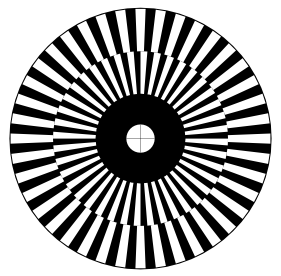
\includegraphics[width=0.3\textwidth]{figs/encoderdisk.png}
		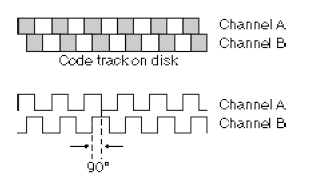
\includegraphics[width=0.3\textwidth]{figs/quadraturencoder.png}
		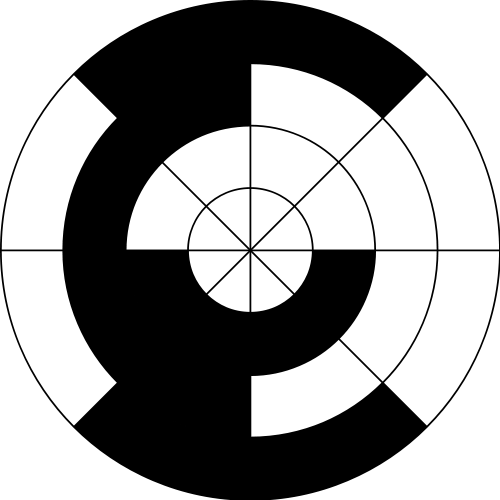
\includegraphics[width=0.3\textwidth]{figs/absoluteencoder.png}
	\caption{From left to right: encoder pattern used in a quadrature encoder, resulting sensor signal (forward motion), absolute encoder pattern (gray coding).}
	\label{fig:encoders}
\end{figure}

While a single sensor would be sufficient to detect rotation and its speed, it does not allow for the determining the direction of motion. Quadrature encoders therefore have two sensors, A and B, that register an interleaving pattern with distance of a quarter phase. If A leads B, for example, the disk is rotating in a clockwise direction. If B leads A, then the disk is rotating in a counter-clockwise direction. It is also possible to create absolute encoders, an example of which is shown in Figure \ref{fig:encoders}, right. This pattern encodes 3-bits, encoding 8 different segments on a disc. Notice that the pattern is arranged in such a way that there is only one bit changing from one segment to the other. This is known as ``Gray code''\index{Gray code}. The function of linear encoders is analogous, both for incremental and absolute encoders.

If combined with a spring, such as in a series elastic actuator, rotary and linear encoders can be used as simple force/torque sensors using Hooke's law ($F=kx$, force equals distance times spring constant). Whereas the series elastic actuator is the most illustrative examples, most load cells operate on the premise of measuring displacements within materials of known properties. Here, measuring changes in resistance or capacitance might be easier choices.

Other means of measuring the actual force at the end-effector or joint torques is measuring the actual current consumed at each joint. Knowing a mechanism's pose allows to calculate the resulting forces and torques across the mechanism as well as the currents required for empty loading conditions. Derivations of these then correspond to additional forces that can hence be calculated.

Finally, there are other means of proprioception, such as simple sensors that can detect when a robot gets picked up, e.g.
 
\section{Sensors using light}
The small form factor and low price of light-sensitive semi-conductors have led to a proliferation of light-based sensing relying on a multitude of physical effects. These include reflection, phase shift, and time of flight.

\subsection{Reflection}
Reflection is one of the principles that is easiest to exploit: the closer an object is, the more it reflects light shined at it. This allows to easily measure distance to objects that reflect light well and are not too far away. In order to make these sensors as independent from an object's color (but unfortunately not totally independent), infrared is most commonly chosen. A distance sensor is made from two components: an emitter and a receiver. They work by emitting an infrared signal and then measuring the strength of the reflected signal. A typical response is shown in Figure \ref{fig:epuckir}. The values obtained at an analog-digital converter correspond to the voltage at the infrared receiver and are saturated for low distances (flat line), and quadratically fall off thereafter.

\begin{figure}
	\centering
		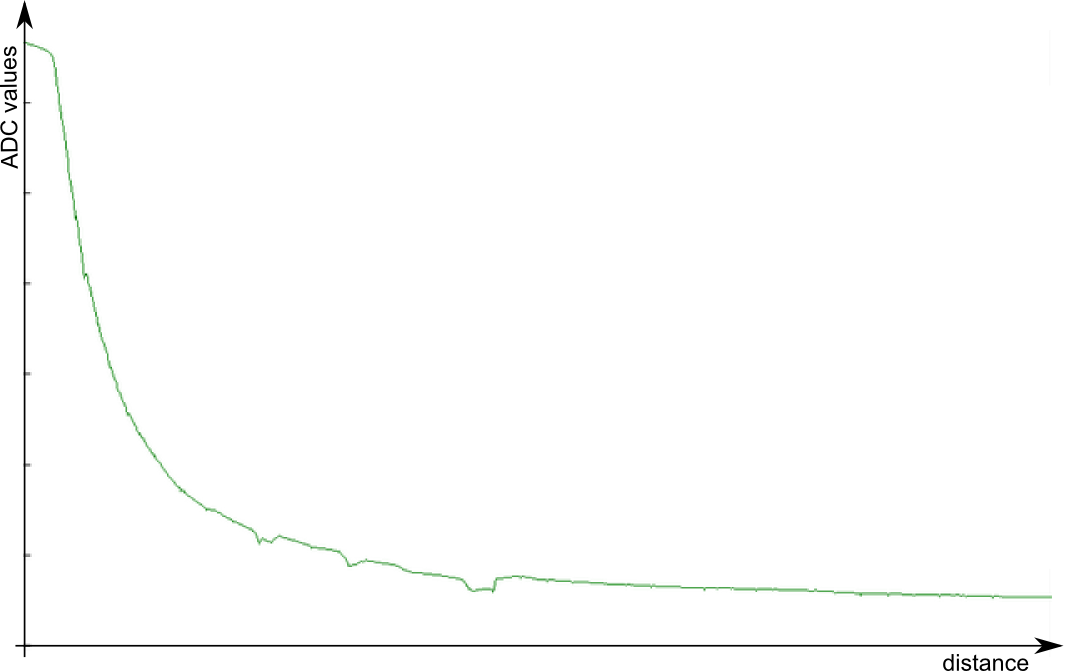
\includegraphics[width=0.8\textwidth]{figs/epuckirsensor.png}
	\caption{Typical response of an infrared distance sensor as a function of distance. Units are left dimensionless intensionally.}
	\label{fig:epuckir}
\end{figure}

When using more than one infrared sensor/emitter pair, e.g., using a camera and a projector, not only allows to measure the distance of many points at once, but also to assess the structure of the environment by calculating its impact on the deformation of patterns. For example a straight line becomes a curve when projected onto a round surface. This approach is known as \emph{structured light}\index{Structured light} and illustrated in Figure \ref{fig:struclight}. Thanks to the continuously increasing efficiency of computational systems, a light-weight version of such an approach has become feasible to be implemented at small scale and low cost at around 2010, and emerged as a novel standard in robotic sensing.

\begin{figure}
	\centering
		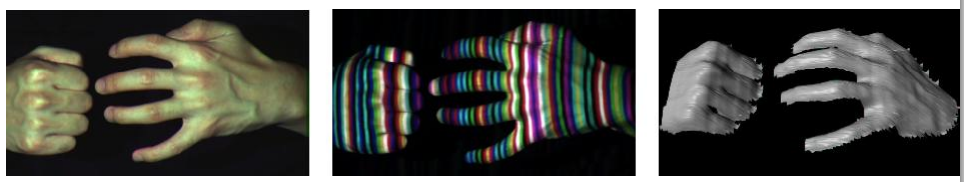
\includegraphics[width=\textwidth]{figs/structuredlight.png}
	\caption{From left to right: two complex physical objects, a pattern of colored straight lines and their deformation when hitting the surfaces, reconstructed 3D shape. From \protect\cite{zhang2002rapid}.}
	\label{fig:struclight}
\end{figure}

Instead of using line patterns, infrared-based depth image sensors use a speckle pattern (a collection of randomly distributed dots with varying distances), and two computer vision concepts: \emph{depth from focus} and \emph{depth from stereo}.\index{Depth from Focus}\index{Depth from Stereo} When using a lens with a narrow focal depth, objects that are closer or farther away appear blurred (you can easily observe this on professional portrait photos, which often use this effect for aesthetic purposes). Measuring the ``bluriness'' of a scene (for known camera parameters) therefore allows for an initial estimate of depth. Depth from stereo instead works by measuring the disparity of the same object appearing in two images taken by cameras that are a known distance apart. Being able to identify the same object in both frames allows to calculate this disparity, and from there the distance of the object. (The farther the object is away, the smaller is the disparity.) This is where the speckle pattern comes in handy, which simply requires to search for blobs with similar size that are close to each other.


\subsection{Phase shift}\label{sec:phaseshiftsensors}
As you can see in Figure \ref{fig:epuckir}, reflection can only be precise if distances are short. Instead of measuring the strength (aka amplitude) of the reflected signal, laser distance sensors measure the phase difference of the reflected wave. In order to do this, the emitted light is modulated with a wave-length that exceeds the maximum distance the scanner can measure. If you would use visible light and do this much slower, you would see a light that keeps getting brighter, then getting darker, briefly turns off and then starts getting brighter again. Thus, if you would plot the amplitude, i.e. its brightness, of the emitted signal vs. time you would see a wave that has zero-crossings when the light is dark. As light travels with the speed of light, this wave propagates through space with a constant distance (the wavelength) between its zero crossings. When it gets reflected, the same wave travels back (or at least parts of it that get scattered right back). For example, modern laser scanners\index{Laser range finder} emit signals with a frequency of 5 MHz (turning off 5 million times in one second). Together with the speed of light of approximately 300,000km/s, this leads to a wavelength of 60m and makes such a laser scanner useful up to 30m.

When the laser is now at a distance that corresponds exactly to one half the wave-length, the reflected signal it measures will be dark at the exact same time its emitted wave goes through a zero-crossing. Going closer to the obstacle results in an offset that can be measured. As the emitter knows the shape of the wave it emitted, it can calculate the phase difference between emitted and received signal. Knowing the wave-length it can now calculate the distance. As this process is independent from ambient light (unless it has the exact same frequency as the laser being used), the estimates can be very precise. This is in contrast to a sensor that uses signal strength. As the signal strength decays at least quadratically, small errors, e.g. due to fluctuations in the power supply that drives the emitting light, noise in the analog-digital converter, or simply differences in the reflecting surface have drastic impact on the accuracy and precision (see below for a more formal definition of this term). 

As the laser distance measurement process is fast, such lasers can be combined with rotating mirrors to sweep larger areas, known as \emph{Laser Range Scanners}\index{Laser Range Scanners}. Such systems have been combined into packages consisting of up to 64 scanning lasers, providing a depth map around a car while driving, e.g. It is also possible to modulate projected images with a phase-changing signal, which is the operational principle of early ``time-of-flight'' cameras, which is not an accurate description of their operation, however

\subsection{Time-of-flight}
The most precise distance measurements light can provide is by measuring its time of flight. This can be done by counting the time a signal from the emitter becomes visible in the receiver. As light travels very fast (3,000,000,000m/s), this requires high-speed electronics that can measure time periods smaller than nano-seconds in order to achieve centimeter accuracy. In practice this is done by combining the receiver with a very fast (electronic) shutter that operates at the same frequency with which light is emitted. As this timing is known, one can infer the time light must have been traveling by measuring the quantity of photons that have made it back from the reflective surface within one shutter period. Considering a concrete example, light travels 15m in 50ns. Therefore, it will take a pulse 50ns to return from an object at a distance of 7.5m. If the camera sends out a pulse of 50ns length and then closes the receiver with a shutter, the receiver will receive more photons the closer the object is, but no photons if the object is farther away than 7.5m. Given a fast enough and precise circuit that acts as a shutter, it is sufficient to measure the actual amount of light that returns from the emitter.

\section{Sensors using sound}
\subsection{Ultra-sound distance sensors}
Ultra-sound distance sensor: An ultra-sound distance sensor operates by emitting an ultra-sound pulse and measures its reflection. Unlike a light-based sensor that measures the amplitude of the reflected signal, a sound-based sensor measures the time it took the sound to travel. This is possible, because sound travels at much lower speed (300m/s) than light (300,000km/s). The fact that the sensor actually has to wait for the signal to return leads to a trade-off between range and bandwidth. (Look these definitions up above before you read on.) In other words, allowing a longer range requires waiting longer, which in turn limits how often the sensor can provide a measurement. Although US distance sensors have become less and less common in robotics, they have an advantage over light-based sensors: instead of sending out a ray, the ultra-sound pulse results in a cone with an opening angle of 20 to 40 degrees. By this, US sensors are able to detect small obstacles without the requirement of directly hitting them with a ray. This property makes them the sensor of choice in automated parking helpers in cars.

\subsection{Texture recognition}
Audible sound consists of high frequency vibrations in the range between 20 Hz and roughly 15 kHz. Microphones are therefore ideally suited to measure vibrations in this range. This allows them to double as the Pascinian corpuscle in human skin cells, which is known to have a resonance frequency of 250 Hz and is mostly responsible for texture recognition. Indeed, rubbing a texture against a microphone can indeed be used for differentiating between tens and hundreds of different textures \cite{hughes14}, with a number of commercial sensors available. These sensors usually calculate the frequency spectrum of the recorded signal, which can then be classified using machine learning techniques. Being able to recognize a texture by touch is important in applications like grasping and navigation through cluttered terrain.  

\section{Inertia-based sensors}
A moving mass does not loose its kinetic energy, but for friction. Likewise, a resting mass will resist acceleration. Both effects are due to ``inertia'' \index{Inertia} and can be exploited to measure acceleration and speed. 

\subsection{Accelerometer}
An accelerometer \index{Accelerometer}can be thought of as a mass on a dampened spring. Considering a vertical spring with a mass hanging down from it, we can measure the acting force $F=kx$ (Hooke's law) \index{Hooke's law}by measuring the displacement $x$ that the mass has stretched the spring. Using the relationship $F=am$, we can now calculate the acceleration $a$ on the mass $m$. On earth, this acceleration is roughly $9.81\frac{kg m}{s^2}$. In practice, these spring/mass systems are realized using microelectromechanical systems (MEMS), such as a cantilevered beam whose displacement can be measured, e.g., using a capacitive sensor. Accelerometers measure up to three axes of translational accelerations. Infering a position from this requires integration twice, thereby amplifying any noise, making position estimates using accelerometers alone infeasible. As gravity provides a constant acceleration vector, accelerometers are very good at estimating the pose of an object with respect to gravity.

\subsection{Gyroscopes}
A gyroscope is an electro-mechanical device that can measure rotational orientation. It is complementary to the accelerometer that measures translational acceleration. Classically, a gyroscope consists of a rotating disc that could freely rotate in a system of pivots and gimbals. When moving the system, the inertial momentum keeps the original orientation of the disc, allowing to measure the orientation of the system relative to where the system was started. A variation of the gyroscope is the rate gyro, which measures rotational speed. 

What a rate gyro \index{Rate gyro}\index{Gyroscopes} measures can most intuitively be illustrated by considering the implementation of an \emph{optical} rate gyro. In an optical gyro, a laser beam is split into two beams and send around a circular path in two opposite directions. If this setup is rotated against the direction of one of these laser beams, one laser will have to travel slightly longer than the other, leading to a measurable phase-shift at the receptor. This phase shift is proportional to the \emph{rotational speed} of the setup. As light with the same frequency and phase will add, and lights with the same frequency but opposite phases will cancel each other, light at the detector will be darker for high rotational velocities. As small-scale optical rate gyros are not practical for multiple reasons, MEMS rate gyros rely on a mass suspended by springs. The mass is actively vibrating, making it subject to Coriolis forces, when the sensor is rotated. Coriolis forces can be best understand by moving orthogonally to the direction of rotation on a vinyl disk player. In order to move in a straight line, you will not only need to move forwards, but also sideways. The necessary acceleration to change the speed of this sideway motion is counteracting the Coriolis force, which is both proportional to the lateral speed (the vibration of the mass in a MEMS sensor) and the rotational velocity, which the device wishes to measure. Note that the MEMS gyro would only be able to measure acceleration if it were not vibrating.

Gyroscopes can measure the rotational speed around three axes, which can be integrated to obtain absolute orientation. As an accelerometer measures along three axes of translation, the combination of both sensors can provide information on motion in all six degrees of freedom. Together with a magnetometer (compass), which provides absolute orientation, his combination is also known as \emph{Inertial Measurement Unit} (IMU), \index{Inertial Measurement Unit}\index{IMU}.

\section{Beacon-based sensors}
Localizing an object by triangulation goes back to ancient civilizations orienting themselves using the stars. As stars are only visible during unclouded nights, seafarers have eventually invented systems of artificial beacons emitting light, sound, and eventually radio waves. The most sophisticated of such systems is the Global Positioning System (GPS). GPS consists of a number of satellites in orbit, which are equipped with knowledge about their precise location and have synchronized clocks. These satellites broadcast a radio signal that travels at the speed of light and is coded with its time of emission. GPS receivers can therefore calculate the distance to each satellite by comparing time of emission and time of arrival. As not only the position (x,y,z), but also the time difference between the GPS receiver's clock and the synchronized clocks of the satellites is unknown, four satellites are needed to obtain a ``fix''. Due to the way information from the satellites is coded, getting an initial fix can take in the order of minutes, but eventually is available multiple times a second. GPS measurements are neither precise nor accurate enough (see below) for small mobile robots, and require to be combined with other sensors, such as IMUs and compasses. (The bearing shown on some GPS receivers is calculated from subsequent positions and is therefore meaningless if the robot is not moving.) 

There exist also a variety of indoor-GPS solutions, which consists of either active or passive beacons that are mounted in the environment at known locations. Passive beacons, for example infrared reflecting stickers arranged in a certain pattern or 2D barcodes, can be detected using cameras and their pose can be calculated from their known dimensions. Active beacons instead usually emit radio, ultrasound or a combination thereof, which can then be used to estimate the robot's range to this beacon. 
  
\section{Terminology}
It is now time to introduce  a more precise definition of terms such as ``speed'' and ``resolution", as well as additional taxonomy that is used in a robotic context. %Roboticists differentiate between proprioceptive and exteroceptive sensors. Proprioceptive sensors measure quantities that are internal to the robot such as wheel-speed, current consumption, joint position or battery status. Exteroceptive sensors measure quantities from the environment, such as distance to a wall, the strength of ambient light or the pattern of a picture at the wall.

Roboticists differentiate between \emph{active} and \emph{passive} sensors. Active sensors \index{Active sensor} emit energy of some sort and measure the reaction of the environment. Passive sensors \index{Passive sensor} instead measure energy from the environment. For example, most distance sensors are active sensors (as they sense the reflection of a signal they emit), whereas an accelerometer, compass, or a push-button are passive sensors.

The difference between the upper and the lower limit of the quantity a sensor can measure its known as its \emph{range} \index{Range (sensor)}. This should not be confused with the \index{Dynamic Range (sensor)} \emph{dynamic range}, which is the ratio between the lowest and highest value a sensor can measure. It is usually expressed on a logarithmic scale (to the basis 10), also known as ``decibel''\index{Decibel}. The minimal distance between two values a sensor can measure is known as its \index{Resolution (sensor)} \emph{resolution}. The resolution of a sensor is given by the device physics (e.g., a light detector can only count multiples of a quant), but usually limited by the analog-digital conversion process. The resolution of a sensor should not be confused with its accuracy or its precision (which are two different concepts). For example, whereas an infrared distance sensor might yield 4096 different values to encode distances from 0 to 10cm, which suggests a resolution of around 24 micrometers, its precision is far above that (in the order of millimeters) due to noise in the acquisition process.

Technically, a sensors accuracy \index{Accuracy (sensor)} is given by the difference between a sensors (average) output $m$ and the true value $v$:
\begin{equation}
accuracy=1-\frac{|m-v|}{v}
\end{equation}
A sensor's precision \index{Precision (sensor)} instead is given by the ratio of range and statistical variance of the signal. Precision is therefore a measure of repeatability of a signal, whereas accuracy describes a systematic error that is introduced by the sensor physics. This is illustrated in Figure \ref{fig:precision}.
\begin{figure}
	\centering
		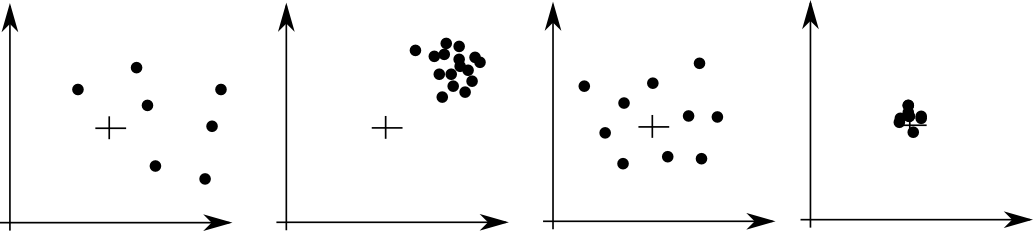
\includegraphics[width=0.9\textwidth]{figs/precisionvsaccuracy.png}
	\caption{From left to right, the cross corresponds to the true value of the signal: neither precise nor accurate, precise, but not accurate, accurate, but not precise, and accurate and precise. 
	\label{fig:precision}}
\end{figure}

A GPS sensor is usually precise within a few meters, but only accurate to tens of meters. This becomes most obvious when satellite configurations change, resulting in the precise region jumping by a couple of meters. In practice, this can be avoided by fusing this data with other sensors, e.g. from an IMU.

The speed at which a sensor can provide measurements is known as its \index{Bandwidth (sensor)} \emph{bandwidth}. For example, if a sensor has a bandwidth of 10 Hz, it will provide a signal ten times a second. This is important to know, as querying the sensor more often is a waste of computational time and potentially misleading.


\section*{Take-home lessons}
\begin{itemize}
\item Most of a robot's sensors either address the problem of robot localization or localizing and recognizing objects in its vicinity.
\item Each sensors has advantages and drawbacks that are quantified in its range, precision, accuracy, and bandwidth. Therefore, robust solutions to a problem can only be achieved by combining multiple sensors with differing operation principles.
\item Solid-state sensors (i.e. without mechanical parts) can be miniaturized and cheaply manufactured in quantity. This has enabled a series of affordable IMUs and 3D depth sensors that will provide the data basis for localization and object recognition on mass-market robotic systems
\end{itemize} 

\section*{Exercises}\small
\begin{enumerate}
\item Given a laser scanner with an angular resolution of 0.01 rad and a maximum range of 5.6 meters, what is the minimum range $d$ a robot needs to have from an object of 1cm width to definitely sense it, i.e., hit it with at least one of its rays? You can approximate the distance between two rays with the arc length. 
\item Why does the bandwidth of a Ultra-sound based distance sensor decreases significantly when increasing its dynamic range, but that of a laser range scanner does not for typical operation?
\item You are designing an autonomous electric car to transport goods on campus. As you are worried about cost, you are thinking about whether to use a laser scanner or an ultra-sound sensor for detecting obstacles. As you drive rather slow, you are required to sense up to 15 meters. The laser scanner you are considering can sense up to this range and has a bandwidth of 10Hz. Assume 300m/s for the speed of sound in the following.
\begin{enumerate}
\item Calculate the time it takes until you hear back from the US sensor when detecting an obstacle 15m away. Assume that the robot is not moving at this point.
\item Calculate the time it takes until you hear back from the laser scanner. Hint: you don’t need the speed of light for this, the answer is in the specs above.      
\item Assume now that you are moving toward the obstacle. Which sensor will give you a measurement that is closer to your real distance at the time of reading and why? 
\end{enumerate}
\end{enumerate}\normalsize
\chapter{Vision}\label{chap:vision}
Vision is one of the information-rich sensor system both humans and robots have available. Processing the wealth of information that is generated by vision sensors is still a key challenge, however. The goal of this chapter is to introduce
\begin{itemize}
\item images as two-dimensional signals,
\item providing an intuition of the wealth of information hidden in low-level information,
\item introducing basic convolution and threshold-based image processing algorithms.
\end{itemize}

\section{Images as two-dimensional signals}
Images are captured by cameras containing matrices of charge-coupled devices (CCD) or similar semi-conductors that can turn photons into electrical signals. These matrices can be read out pixel by pixel and turned into digital values, for example an array of 640 by 480 three-byte tuples corresponding to the red, green, and blue (RGB) components the camera has seen. An example of such data, for simplicity only one color channel, is shown in Figure \ref{fig:iss_closeup}. 

Looking at the data clearly reveals the white tile within the black tiles at the lower-right corner of the chessboard. Higher values correspond to brighter colors (white) and lower values to darker colors. We also observe that although the tiles have to have the same color, the actual values differ quite a bit. It might make sense to think about these values much like we would do if the data would be 1D signal: taking the ``derivative'', e.g., along the horizontal rows, would indicate areas of big changes, whereas the ``frequency'' of an image  would indicate how quickly values change. Areas with smooth gradients, e.g., black and white tiles, would then have low frequencies, whereas areas with strong gradients, would contain high frequency information. 

\begin{figure}[!htb]
	\centering
		\includegraphics[width=\textwidth]{figs/iss_closeupmatrix}
	\caption{A chessboard floating inside the ISS, astronaut Gregory Chamitoff. The inset shows a sample of the actual data recorded by the image sensor. One can clearly recognize the contours of the white tile.}
	\label{fig:iss_closeup}
\end{figure}

This language opens the door to a series of signal processing concepts, such as low-pass filters (supressing high frequency information), high-pass filters (suppressing low frequency information), or band-pass filters (letting only a range of frequencies pass), analysis of the frequency spectrum of the image (the distribution of content at different frequencies), or ``convolving'' the image with another two-dimensional function. The next sections will provide both an intuition of what kind of meaningful information is hidden in such abstract data and provide concrete examples of signal processing techniques that make this information appear.

\section{From signals to information}
Unfortunately, many phenomena that often have very different or even opposite meaning look very similar when looking at the low-level signal. For example, drastic changes in color values do not necessarily mean that the color of a surface indeed has changed. Similar patterns are generated by depth discontinuities, specular highlights, changing lighting conditions, or surface orientation changes. These examples are illustrated in Figure \ref{fig:iss_edges} and make computer vision a hard problem.  

\begin{figure}[!htb]
	\centering
		\includegraphics[width=\textwidth]{figs/iss_edges}
	\caption{Inside of the international space station (left), highlighted areas in which pixel values change drastically (right). Underlying effects that produce similar responses: change in surface properties (1), depth discontinuities (2), specular highlights (3), changing lighting conditions such as shadows (4), or surface orientation changes (5).
	\label{fig:iss_edges}}
\end{figure}

This example illustrates that signals alone are not sufficient to understand a phenomenon, but require context. Here, the context does not only refer to surrounding signals, but also high-level conceptional knowledge such as the fact that light sources create shadows and specular highlights, that objects in the front appear larger, and so on. How important such conceptional knowledge is, is illustrated by Figure \ref{fig:craters}.

Both images show an identical landscape that once appears to be speckled with craters, once with bubble-like hills. At first glance, both scenes are illuminated from the left, suggesting a change in the landscape. Once information that the sun is illuminating one picture from the left and the other from the right, however, it becomes clear that the craters are simply differently illuminated and what we perceive as bumps eventually turns back into craters. 

\begin{figure}[!htb]
	\centering
		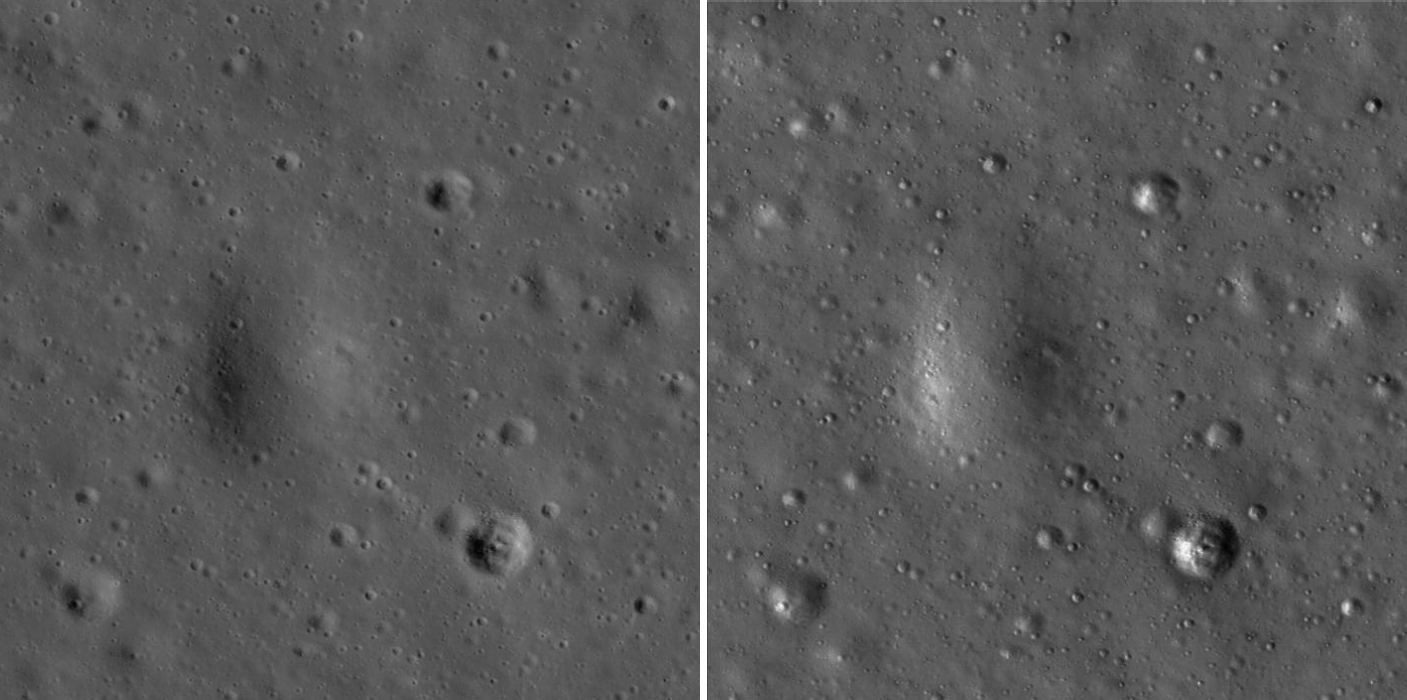
\includegraphics[width=\textwidth]{figs/craters}
	\caption{Picture of the Apollo 15 landing site during different times of the day. The landscape is identical, but appears to be speckled with craters (lift) or hills (right). Knowing that the sun is illuminating the scene from the left and right, respectively, does explain this effect. Image credit: NASA/GSFC/Arizona State University.
	\label{fig:craters}}
\end{figure}

More surprisingly, conceptual knowledge is often sufficient to make up for the lack of low-level cues in an image. An example is shown in Figure \ref{fig:dalmatian}. Here, a Dalmatian dog can be clearly recognized despite absence of cues for its outline, simply by extrapolating its appearance and pose from conceptual knowledge. 

These examples illustrate both the advantages and drawbacks of a signal processing approach. While an algorithm will detect interesting signals even there where we don't see, or don't expect them (due to conceptional bias), image understanding not only requires low-level processing, but intelligent combination of the low-level cue's spatial relationship and conceptual knowledge about the world. 


\begin{figure}
	\centering
		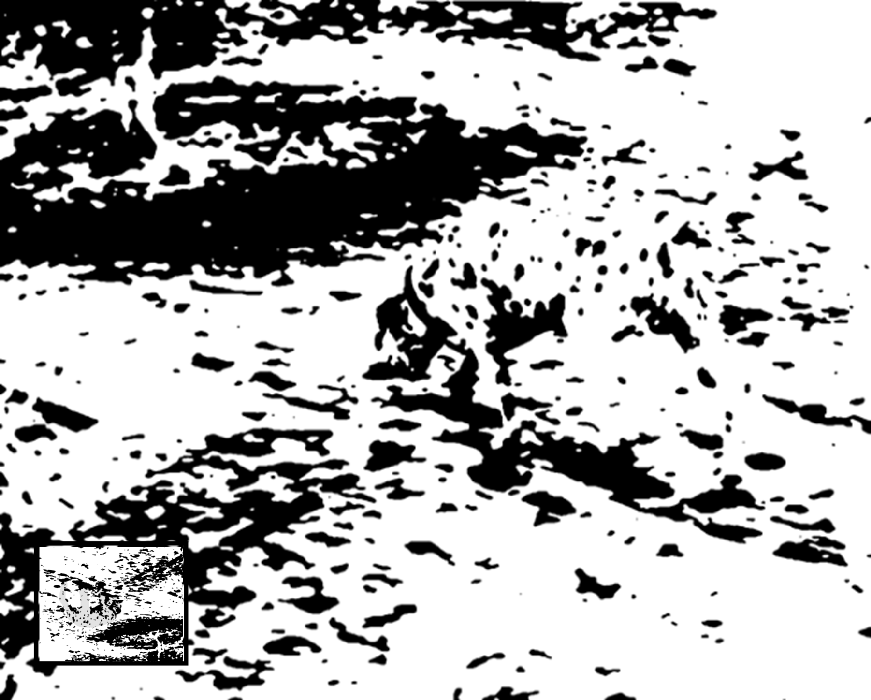
\includegraphics[width=\textwidth]{figs/dalmatian}
	\caption{The image of a Dalmatian dog can be clearly recognized by most spectators even though low-level cues such as edges are only present for ears, chin and parts of the legs. The contours of the animals are highlighted in a flipped version of the image in the inset.
	\label{fig:dalmatian}}
\end{figure}

\section{Basic image operations}
Basic image operations can be thought of as a filter that operates in the frequency or in the space (color) domain. Although most filters directly operate in the color domain, knowing how they affect the frequency domain is helpful in understanding the filter's function. For example, a filter that is supposed to highlight edges, such as shown in Figure \ref{fig:iss_edges} should suppress low frequencies, i.e., areas in which the color values do not change much, and amplify high-frequency information, i.e., areas in which the color values change quickly. The goal of this section is to provide a basic understanding of how basic image processing operation works. The methods presented here, while still valid, have been superseded by more sophisticated implementations that are widely available as software packages or within desktop graphic software.

\subsection{Convolution-based filters}
 A filter can be implemented using the \emph{convolution} \index{Convolution} operator that convolves function $f()$ with function $g()$. 
\begin{equation}
f(x)\star g(x)=\int_{-\infty}^{\infty}f(\tau)g(x-\tau)d\tau
\end{equation}
We then call function $g()$ a \emph{filter}\index{Filter}. As will become more clear further below, the convolution literally shifts the function $g()$ across the function $f()$ while multiplying the two. As images are discrete signals, the convolution is usually discrete
\begin{equation}
f[x]\star g[x]=\sum_{i=-\infty}^{\infty}f[i]g[x-i]
\end{equation} 
For 2D signals, like images, the convolution is also two-dimensional:
\begin{equation}\label{eq:2dconv1}
f[x,y]\star g[x,y]=\sum_{i=-\infty}^{\infty}\sum_{j=-\infty}^{\infty}f[i,j]g[x-i,y-j]
\end{equation}
Although we have defined the convolution from negative infinity to infinity, both images and filters are usually finite. Images are constrained by their resolution, and filters are usually much smaller than the images themselves. Also, the convolution is commutative, therefore (\ref{eq:2dconv1}) is equivalent to 
\begin{equation}\label{eq:2dconv2}
f[x,y]\star g[x,y]=\sum_{i=-\infty}^{\infty}\sum_{j=-\infty}^{\infty}f[x-i,y-j]g[i,j].
\end{equation}

\subsubsection{Gaussian smoothing}
A very important filter is the Gaussian filter.\index{Gaussian filter} It is shaped like the Gaussian bell function and can be easily stored in a 2D matrix. Implementing a Gaussian filter is surprisingly simple, e.g., such as
\begin{equation}
g(x,y)=\frac{1}{10}
\left(
\begin{array}{ccc}
1 & 1 & 1\\
1 & 2 & 1\\
1 & 1 & 1\\
\end{array}
\right)
\end{equation}
Using this filter in Equation \ref{eq:2dconv2} on an infinitely large image $f()$ leads to
\begin{equation}\label{eq:2dconv3}
f[x,y]\star g[x,y]=\sum_{i=-1}^{1}\sum_{j=-1}^{1}f[x-i,y-j]g[i,j]
\end{equation}
(assuming $g(0,0)$ addresses the center of the matrix). What now happens is that each pixel $f(x,y)$ becomes the average of that of its neighbors, with its previous value weighted twice (as $g(0,0)=0.2$) that of their neighbors. More concretely,
\begin{equation}
\tiny
f(x,y)=
\begin{array}{lll}
f(x+1,y+1)g(-1,-1) &+f(x+1,y)g(-1,0) &+f(x+1,y-1)g(-1,1)\\
+f(x,y+1)g(0,-1) &+f(x,y)g(0,0) &+f(x,y-1)g(0,1)\\
+f(x-1,y+1)g(1,-1) &+f(x-1,y)g(1,0) &+f(x-1,y-1)g(1,1)
\end{array}
\end{equation}
Doing this for all $x$ and all $y$ literally corresponds to sliding the filter $g()$ along the image. 

\begin{figure}
	\centering
		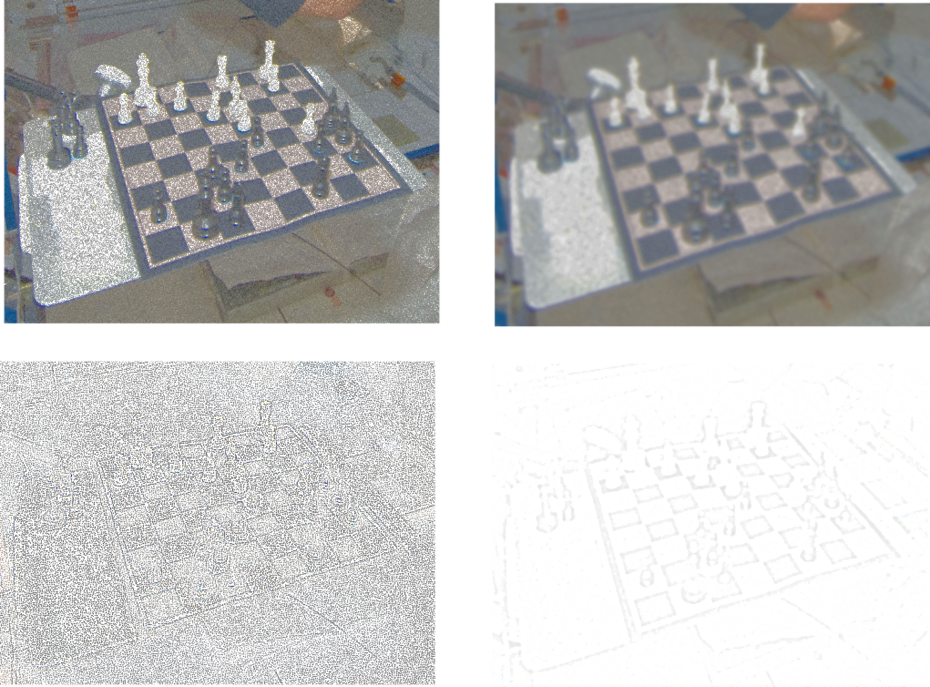
\includegraphics[width=\textwidth]{figs/filters}
	\caption{A noisy image before (top left) and after filtering with a Gaussian kernel (top right). Corresponding edge images are shown underneath. 
	\label{fig:filters}}
\end{figure}

An example of filter $g(x,y)$ in action is shown in Figure \ref{fig:filters}. The filter acts as a \emph{low-pass filter} \index{Low-pass filter}, suppressing high frequency components. Indeed, noise in the image is suppressed, leading also to a smoother edge image, which is shown underneath.

\subsubsection{Edge detection}\label{sec:sobel}
Edge detection can be achieved using another convolution-based filter, the \emph{Sobel} kernel\index{Sobel filter}
\begin{equation}
s_x(x,y)=
\left(
\begin{array}{ccc}
-1 & 0 & 1\\
-2 & 0 & 2\\
-1 & 0 & 1\\
\end{array}
\right)
\qquad
s_y(x,y)=
\left(
\begin{array}{ccc}
1 & 2 & 1\\
0 & 0 & 0\\
-1 & -2 & -1\\
\end{array}
\right)
\end{equation}
Here, $s_x(x,y)$ can be used to detect vertical edges, whereas $s_y(x,y)$ highlights horizontal edges. Edge detectors, such as the \emph{Canny} edge detector\index{Canny edge detector}  therefore run at least two of such filters over an image to detect both horizontal and vertical edges.

\subsubsection{Difference of Gaussians}
An alternative method for detecting edges is the \emph{Difference of Gaussians} (DoG) method \index{Difference of Gaussians (DoG)}. The idea is to subtract two images that have each been filtered using a Gaussian kernel with different width. Both filters supress high-frequency information and there difference therefore leads to a \emph{band-pass} filtered signal\index{Band-pass filter}, from which both low and high frequencies have been removed. As such, a DoG filter acts as a capable edge detection algorithm. Here, one kernel is usually four to five times wider than the other, therefore acting as a much stronger filter.

Differences of Gaussians can also be used to approximate the \emph{Laplacian of Gaussian},\index{Laplacian of Gaussian} i.e., the sum of the second derivatives of a Gaussian kernel. Here, one kernel is roughly 1.6 times wider than the other. The band-pass characteristic of DoG and LoGs are important as they highlight high-frequency information such as edges, yet suppress high-frequency noise in the image.


\subsection{Threshold-based operations}
In order to find objects with a certain color or edge intensity, tresholding an image will lead to a binary image that contains ``true-false'' regions that fit the desired criteria. Thresholds make use of operators like $>,<,\leq,\geq$ and combinations thereof. There also exist adaptive versions that would adapt the thresholds locally, e.g., to make up for changing lighting conditions.

Albeit thresholding is deceptively simple, finding correct threshold values is a hard problem. In particular, actual pixel values change drastically with changing lighting conditions and there is no such thing as ``red'' or ``green'' when inspecting the actual values under different conditions. 

\subsection{Morphological Operations}
Another class of filters are morphological operators which consists of a kernel describing the structure of the operation (this can be as simple as an identity matrix) and a rule on how to change a pixel value based on the values in the neighborhood defined by the kernel.

Important morphological operators are \emph{erosion} and \emph{dilation} \index{Erosion}\index{Dilation}. The erosion operator assigns a pixel value with the minimum value that it can find in the neighborhood defined by the kernel. The dilation operator assigns a pixel value with the maximum value it can find in the neighborhood defined by the kernel. This is useful, e.g., to fill holes in a line or remove noise. A dilation followed by an erosion is known as a ``Closing'' and an erosion followed by a dilation as an ``Opening''. Subtracting erosed and dilated images from each other can also serve as an edge detector. Examples of such operators are shown in Figure \ref{fig:morphology}.

\begin{figure}
	\centering
		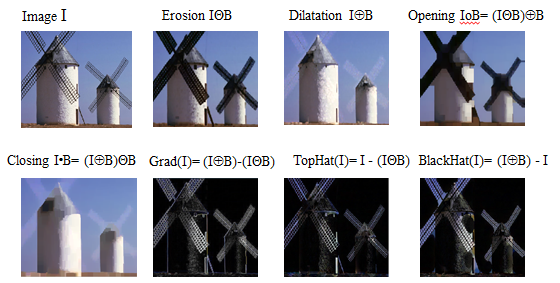
\includegraphics[width=\textwidth]{figs/morphology}
	\caption{Examples of morphological operators erosion and dilation and combinations thereof.
	\label{fig:morphology}}
\end{figure}


\section*{Exercises}\small
\begin{enumerate}
\item Below are shown multiple ``Kernels'' that can be used for convolution-based image filtering. 
\begin{equation}
\nonumber
\begin{array}{|c|c|c}
\hline
1 & 1 & 1\\
\hline
1 & 2 & 1\\
\hline
1 & 1 & 1
\end{array}
\quad
\begin{array}{|c|c|c}
\hline
0 & -1 & 0\\
\hline
0 & -1 & 0\\
\hline
0 & -1 & 0
\end{array}
\quad
\begin{array}{|c|c|c}
\hline
1 & 1 & 1\\
\hline
1 & -4 & 1\\
\hline
1 & 1 & 1
\end{array}
\end{equation}
\begin{enumerate}
\item Identify the Kernel, which can blur an image.
\item What kind of features can be detected by the other two kernels?
\end{enumerate}
\item How many for-loops are needed to implement a 2D convolution? Explain your reasoning.  
\end{enumerate} \normalsize
\chapter{Feature extraction}\label{chap:feature_extraction}
A robot can obtain information about its environment by both active (e.g., ultra-sound, light, and laser) or passive sensing (e.g., acceleration, magnetic field, or cameras). There are only few cases where this information is directly useful to a robot. Before being able to arrive at semantic information such as ``I'm in the kitchen'', ``this is a cup'' or ``this is a horse'', is identifying higher-level \emph{features}.\index{Features} 

The goal of this chapter is to introduce a series of standard feature detectors such as the 
\begin{itemize}
\item Hough-transform to detect lines, circles and other shapes,
\item numerical methods such as least-squares, split-and-merge and RANSAC to find high-level features in noisy data,
\item Scale-invariant features.
\end{itemize}

\section{Feature detection as an information-reduction problem}
The information generated by sensors can be quite formidable. For example, a simple webcam generates 640x480 color pixels (red, green and blue) or 921600 Bytes around 30 times per second. A single-ray laser scanner still provides around 600 distance measurements 10 times per second. This is in contrast to the information that a robot actually requires. Consider for example the maze-solving competition ``Ratslife'' (Section \ref{sec:ratslife}) in which the robot's camera can be used to recognize one of 48 different color patterns (Figure \ref{fig:ratslife}) that are distributed in the environment, or the presence or absence of a charger, essentially reducing hundreds of bytes of camera data to around 6 bit ($2^6=64$ different values) content. The goal of most image processing algorithms is therefore to first reduce information content in a meaningful way and then extract relevant information. In chapter \ref{chap:vision}, we have seen convolution-based filters such as blurring, detecting edges, or binary operations such as thresholding. We are now interested in methods to extract higher-level features such as lines and techniques to extract them.

\section{Features}
Lines are particularly useful features for localization and can correspond to walls in laser scans, markers on the floor or corners detected in a camera image. Whereas a Sobel filter (Section \ref{sec:sobel}) can help us to highlight lines and edges in images, additional algorithms are needed to extract structured information such as the orientation and position of a line with respect to the robot.

A desirable property of a feature is that its extraction is repeatable and robust to rotation, scale, and noise in the data. We need feature detectors that can extract the same feature from sensor data, even if the robot has slightly turned or moved farther or closer to the feature. There are many feature detectors available that accomplish this, prominent examples are the Harris corner detector\index{Harris Corner Detector} (essentially detecting points in the image where vertical and horizontal lines cross) and the SIFT feature detector\index{SIFT features}. Feature detection is important far beyond robotics and is for example used in hand-held cameras that can automatically stitch images together. Here, feature detectors will ``fire'' on the same features in two images taken from slightly different perspectives, which allows the camera to calculate the transformation between the two. 

This chapter focuses on two important classes of features: line features and scale-invariant features in images (SIFT). Both features provide tangible example for the least-squares and RANSAC algorithms, which are also introduced in this chapter. Both features are representative for a large class of detectors, and have been chosen for their simplicity, providing a basis for understanding the function of more complex feature detectors. 

\section{Line recognition}
Why are lines a useful feature? As you will see next chapter, the key challenge in estimating a robot's pose is unreliable odometry, in particular when it comes to turning. Here, a simple infrared sensor measuring the distance to a wall can provide the robot with a much better feel for what actually happened. Similarly, if a robot has the ability to track markers in the environment using vision, it gets another estimate on how much it is actually moving. How information from odometry and other sensors can be fused not only to localize the robot, but also to create maps of its environment, will be the focus of the remainder of this book.

A laser scanner or similar device pointed against a wall will return a suite of $N$ points at position $(x_i,y_i)$ in the robot's coordinate system. These points can also be represented in polar coordinates $ (\rho_i,\theta_i)$. We can now imagine a line running through these points that is parametrized with a distance $r$ and an angle $\alpha$. Here, $r$ is the distance of the robot to the wall and $ \alpha$ its angle. As all sensors are noisy, each point will have distance $d_i$ from the ``optimal'' line running through the points. These relationships are illustrated in Figure \ref{fig:linefitting}.
\begin{figure}
	\centering
		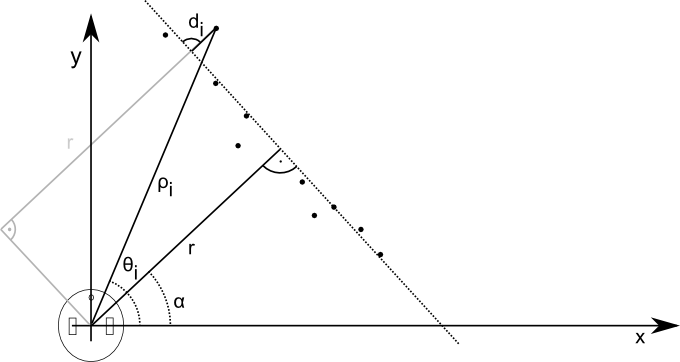
\includegraphics[width=\textwidth]{figs/linefitting.png}
	\caption{A 2D point cloud recorded by a laser-scanner or similar device. A line (dashed) is fitted through the points in a least-square sense.}
	\label{fig:linefitting}
\end{figure}

\subsection{Line fitting using least squares}
Using simple trigonometry we can now write
\begin{equation}
\rho_i \cos(\theta_i-\alpha)-r=d_i.
\end{equation}

Different line candidates --- parametrized by $ r$ and $ \alpha$ --- will have different values for $ d_i$. We can now write an expression for the total error $ S_{r,\alpha}$ as

\begin{equation}
S_{r,\alpha}=\sum_{i=1}^{N}{d_i^2}=\sum_i(\rho_i \cos(\theta_i-\alpha)-r)^2
\end{equation}

Here, we square each individual error to account for the fact that a negative error, i.e.\ a point left of the line, is as bad as a positive error, i.e.\ a point right of the optimal line. In order to optimize $ S_{r,\alpha}$, we need to take the partial derivatives with respect to $ r$ and $ \alpha$, set them zero, and solve the resulting system of equations for $ r$ and $ \alpha$.

\begin{equation}
\frac{\partial{S}}{\partial{\alpha}}=0 \qquad \frac{\partial{S}}{\partial{r}}=0
\end{equation}

Here, the symbol $ \partial$ indicates that we are taking a partial derivative. Solving for $r$ and $\alpha$ is involved, but possible \cite{siegwart2011introduction}:

\begin{equation}\label{eq:linealpha}
\alpha=\frac{1}{2}atan\left(\frac{\frac{1}{N}\sum{\rho_i^2 sin 2\theta_i}-\frac{2}{N^2}\sum{\sum{\rho_i\rho_j cos \theta_i sin \theta_j}}}{\frac{1}{N}\sum{\rho_i^2 cos 2 \theta_i - \frac{1}{N^2}\sum{\sum{\rho_i \rho_j cos(\theta_i+\theta_j)}}}}\right)
\end{equation}

and
\begin{equation}\label{eq:liner}
r=\frac{{\sum \rho_i cos (\theta_i-\alpha)}}{N}
\end{equation}

We can therefore calculate the distance and orientation of a wall captured by our proximity sensors relative to the robot's positions or the height and orientation of a line in an image based on a collection of points that we believe might belong to a line.

This approach is known as the \emph{least-square method}\index{Least-Square Method (Line fitting)} and can be used to fit data to any parametric model. The general approach is to describe the fit between the data and the model in terms of an error. The best fit will minimize this function, which will therefore have a zero derivative at this point. If the result cannot be obtained analytically as in this example, numerical methods have to be used to find the best fit that minimizes the quadratic error.

\subsection{Split-and-merge algorithm}
A key problem with this approach is that it is often unclear how many lines there are and where a line starts and where it ends. Looking through the camera, for example, we will see vertical lines corresponding to wall corners and horizontal ones that correspond to wall-floor intersections and the horizon; using a distance sensor, the robot might detect a corner. We therefore need an algorithm that can separate point clouds into multiple lines. One possible approach is to find the outlier with the strongest deviation from a fitted line and split the line at this point. This is illustrated in Figure \ref{fig:splitandmerge}. This can be done iteratively until each line has no outliers above a certain threshold. 

\begin{figure}
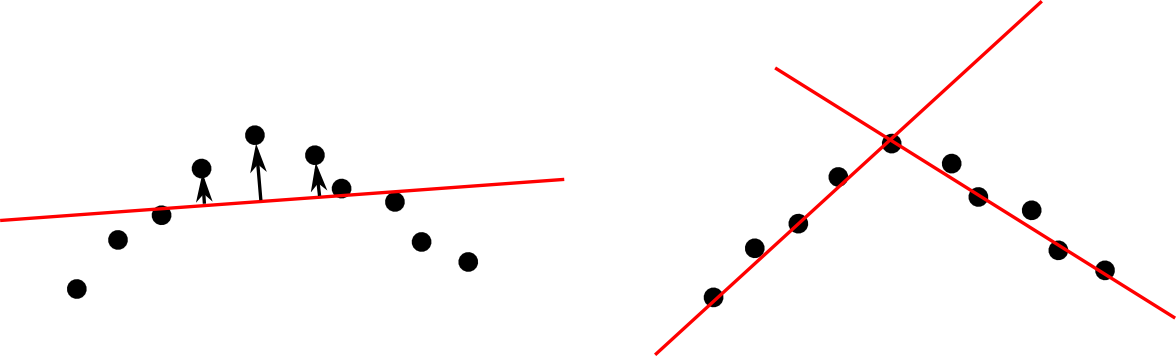
\includegraphics[width=\textwidth]{figs/splitandmerge}
\caption{Split-and-merge algorithm. Initial least-square fit of a line (left). Splitting the data-set at the point with the highest error (after picking a direction) allows fitting two lines with overall lesser error.\label{fig:splitandmerge}} 
\end{figure}

\subsection{RANSAC: Random Sample and Consensus}
If the number of ``outliers'' are large, a least square fit will generate poor results as it will generate the ``best'' fit that accomodates both ``inliers'' and ``outliers''. Also, split-and-merge algorithms will fail as they are extremely susceptive to noise: depending on the actual parameters every outlier will split a potential line into two. A solution to this problem is to randomly sample possible lines and keep those that satisfy a certain desired quality given by the number of points being somewhat close to the best fit. This is illustrated in Figure \ref{fig:ransac}, with darker lines corresponding to better fits. RANSAC\index{RANSAC}\index{Random Sample and Consensus} usually requires two parameters, namely the number of points required to consider a line to be a valid fit, and the maximum $d_i$ from a line to consider a point an inlier and not an outlier. The algorithm proceeds as follows: select two random points from the set and connect them with a line. Grow this line by $d_i$ in both directions and count the number of inliers. Repeat this until one or more lines that have sufficient number of inliers are found, or a maximum number of iterations are reached.

\begin{figure}
\center
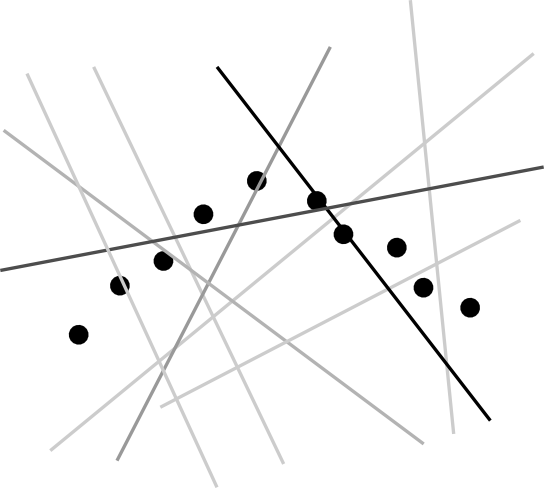
\includegraphics[width=0.6\textwidth]{figs/ransac}
\caption{Random Sample and Consensus (RANSAC). Random lines are evaluated by counting the number of points close by (''inliers''), darker lines are better fits.\label{fig:ransac}} 
\end{figure}

The RANSAC algorithm is fairly easy to understand in the line fitting application, but can be used to fit arbitrary parametric models to any-dimensional data. Here, its main strength is to cope with noisy data.

Given that RANSAC is random, finding a really good fit will take quite some time. Therefore, RANSAC is usually used only as a first step to get an initial estimate, which can then be improved by some kind of local optimization, such as least-squares, e.g.

\subsection{The Hough Transform}
The Hough transform \index{Hough transform} can best be understood as a voting scheme to guess the parametrization of a feature such as a line, circle or other curve \cite{duda1972use}. For example, a line might be represented by $y=mx+c$, where $m$ and $c$ are the gradient and offset. A point in this parameter space (or ``Hough-space'') then corresponds to a specific line in $x-y$-space (or ``image-space''). The Hough-transform now proceeds as follows: for every pixel in the image that could be part of a line, e.g., white pixels in a thresholded image after Sobel filtering, construct all possible lines that intersect this point. (Drawing an image of this would look like a star). Each of these lines has a specifc $m$ and $c$ associated with it, for which we can add a white dot in Hough-space. Continuing to do this for every pixel of a line in an image will yield many $m-c$ pair, but only one that is common among all those pixels of the line in the image: the actual $m-c$ parameters of this line. Thinking about the number of times a point was highlighted in Hough-space as brightness, will turn a line in image space into a bright spot in Hough-space (and the other way round). In practice, a polar representation is chosen for lines. This is shown in Figure \ref{fig:hough}. The Hough transform also generalizes to other parametrization such as circles.  

\begin{figure}
\center
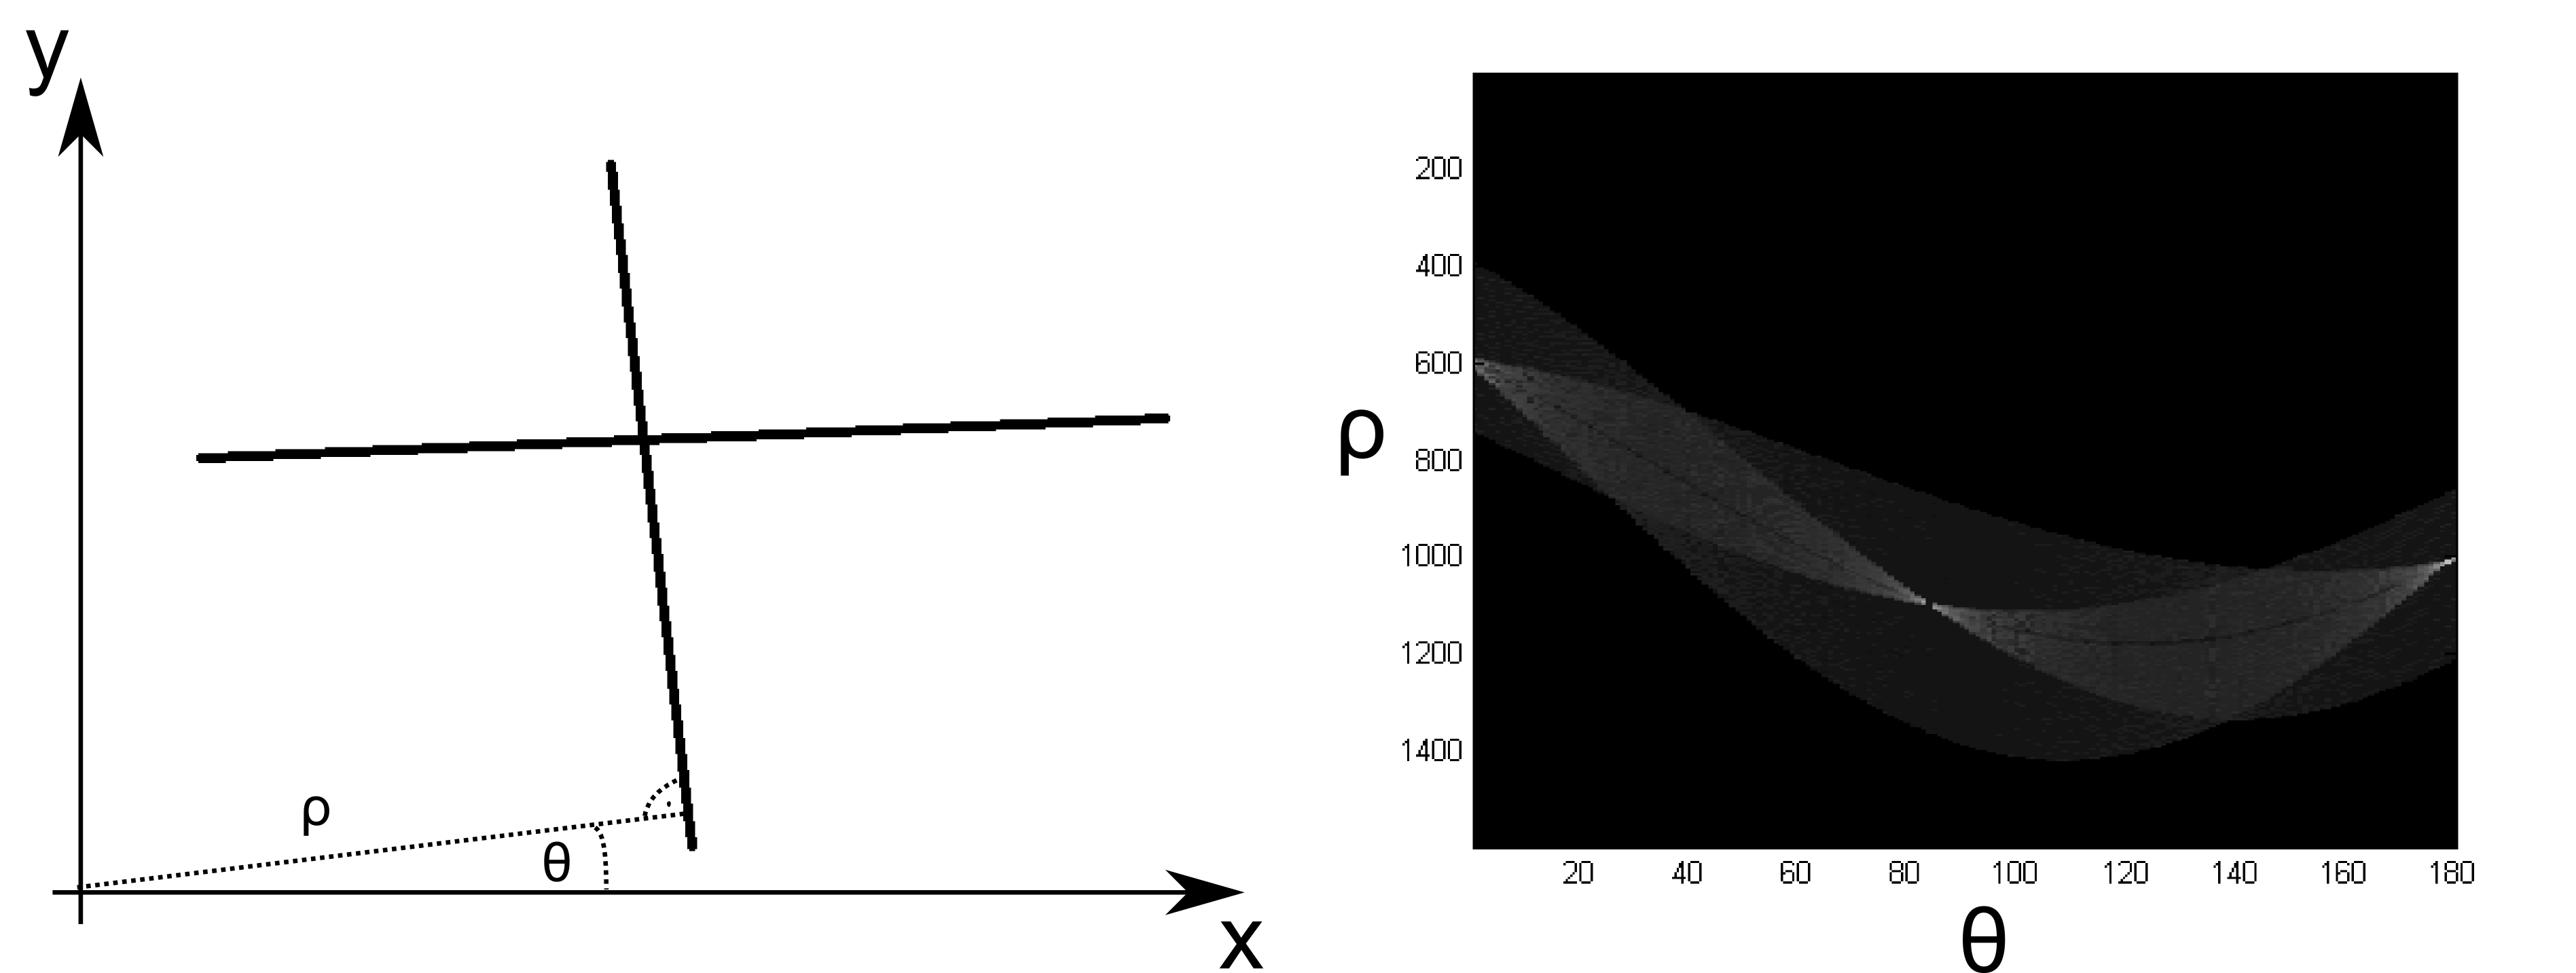
\includegraphics[width=\textwidth]{figs/houghtransform}
\caption{Lines in an image (left) transposed into Hough-space $\rho$ (distance from origin) and $\theta$ (angle of normal with respect to origin). Bright spots in the Hough image (right) correspond to parameters that have received the most ``votes'' and clearly show the two lines at around 90$^o$ and 180$^o$.\label{fig:hough}} 
\end{figure}


\section{Scale-Invariant Feature Transforms}
Scale-invariant feature transforms are a class of algorithms/signal-processing techniques that allow to extract features that are easily detectable across different scales (or distances to an object), independent of their rotation, and to some extent robust to affine transformations, i.e., views of the same object from different perspectives, and illumination changes. The most prominent in this class is the SIFT algorithm \cite{lowe1999object},\index{SIFT} which however has lost popularity due to closed-source and licensing cost, and has been replaced in the past with SURF (Speed-Up Robust Feature)\index{SURF} and many others,  which are freely available and have slightly different performance and varying use cases. As the math behind SURF is more involved, we focus on the intuition behind SIFT and encourage the reader to download and play with the various open-source implementations of other feature detectors that are available open source.

\subsection{Overview}
SIFT proceeds in multiple steps. Descriptions of the algorithm often include its application to object recognition, but these algorithms are independent of feature generation (see below).

\begin{enumerate}
\item Differences of Gaussians (DoG) at different scales:
\begin{itemize}
\item Generate multiple scaled versions of the same image by re-sampling every 2nd, 4th and so on pixel.
\item Filtering each scaled picture with various Gaussian filters of different variance.
\item Calculating the difference between pairs of filtered images. This is equivalent to a DoG filter.
\end{itemize}

\item Detecting local minima and maxima in the DoG images across different scales (Figure \ref{fig:siftrejection}, left) and reject those with low contrast (Figure \ref{fig:siftrejection}, right). 

\begin{figure}
	\centering
		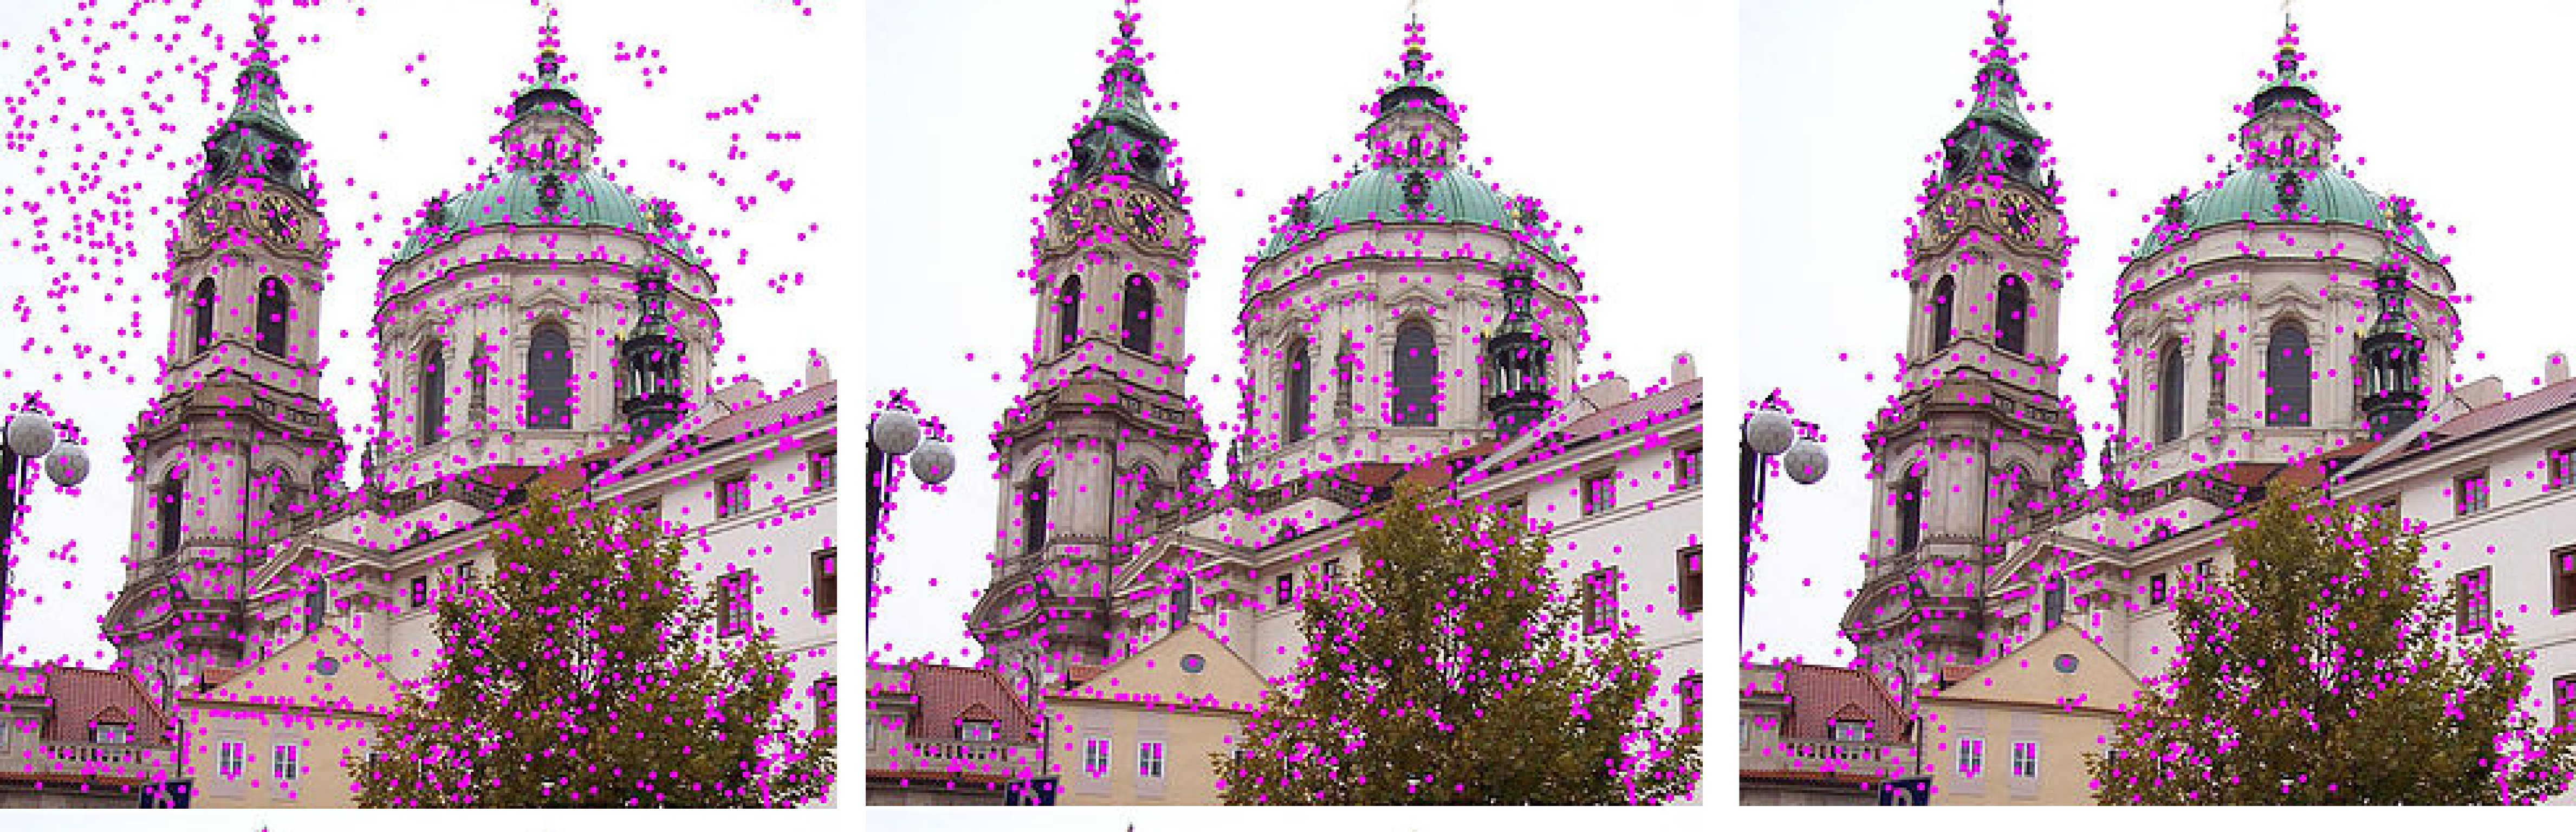
\includegraphics[width=\textwidth]{figs/siftrejection.png}
	\caption{After scale space extrema are detected (left), the SIFT algorithm discards low contrast keypoints (center) and then filters out those located on edges (right). \copyright Lukas Mach CC-BY 3.0}
	\label{fig:siftrejection}
\end{figure}

\item Reject extrema that are along edges by looking at the second derivative around each extrema (Figure \ref{fig:siftrejection}, right). Edges have a much larger principal curvature across them than along them.
\item Assign a ``magnitude'' and ``orientation'' to each remaining extrema (keypoint). The magnitude is the squared difference between neighboring pixels and the orientation is the angle between magnitude along the y-axis vs. magnitude along the x-axis. These calculations are made for all pixels in a fixed neighborhood around the initial keypoint, e.g., in a 16x16 pixel neighborhood.
\item Collect orientations of neighboring pixels in a histogram, e.g., 36 bins each covering 10 degrees. Maintain the orientation corresponding to the strongest peak and associate it with the keypoint.
\item Repeat step 4, but for four 4x4 pixel areas around the keypoint in the image scale that has the most extreme minima/maxima. Here, only 8 bins are used for the orientation histogram. As there are 16 histograms in a 16x16 pixel area, the feature descriptor has 128 dimensions.
\item The feature descriptor vector is normalized, tresholded, and again normalized to make it more robust against illumination changes.
\item Local gradient magnitude and orientation are grouped into bins and create a 128-dimensional feature descriptor.
\end{enumerate}

The resulting 128 dimensional feature vectors are now scale-invariant (due to step 2), rotation-invariant (due to step 5), and robust to illumination changes (due to step 7).

\subsection{Object Recognition using scale-invariant features}
Scale-invariant features of training images can be stored in a database and can be used to identify these objects in the future. This is done by finding all features in an image and comparing them with those in the database. This comparison is done by using the Euclidian distance as metric and searching a k-d tree (with d=128). In order to make this approach robust, each object needs to be identified by at least 3 independent features. For this, each descriptor stores the location, scale and orientation of it relative to some common point on the object. This allows each detected feature to ``vote'' for the position of the object that it is most closely associated with in the database.  This is done using a Hough-transform. For example, position (2 dimensions) and orientation (1 dimension) can be discretized into bins (30 degree width for orientation); bright spots in Hough-space then correspond to an object pose that has been identified by multiple features.

\section*{Take-home lessons}
\begin{enumerate}
\item Features are ``interesting'' information in sensor data that are robust to variations in rotation and scale as well as noise.
\item Which features are most useful depends on the characteristics of the sensor generating the data, the structure of the environment, and the actual application.
\item There are many feature detectors available some of which operating as simple filters, others relying on machine learning techniques.
\item Lines are among the most important features in mobile robotics as they are easy to extract from many different sensors and provide strong clues for localization.
\end{enumerate}

\section*{Exercises}\small
\begin{enumerate}
\item Think about what information would make good features in different operating scenarios: a supermarket, a warehouse, a cave. 
\item What other features could you detect using a Hough transform? Can you find parameterizations for a circle, a square or a triangle?
\item Do an online search for SIFT. What other similar feature detectors can you find? Which provide source code that you can use online?
\item A line can be represented by the function $y=mx+c$. Then, the Hough-space is given by a 2D coordinate system spanned by $m$ and $c$.\begin{enumerate}
\item Think about a line representation in polar coordinates. What components has the Hough-space in this case?
\item Derive a parameterization for a circle and describe the resulting Hough space.
\end{enumerate}
\end{enumerate}
\normalsize
% \chapter{Uncertainty and Error Propagation}
\chapter{不确定性和误差传播}
\label{chap:uncertainty}

% Robots are systems that combine sensing, actuation, computation, and communication. Except for computation, all of its sub-systems are subject to a high degree of uncertainty. This can be observed in daily life: phone calls often are of poor quality, making it hard to understand the other party, characters are difficult to read from far away,  the front wheels of your car slip when accelerating on a rainy road from a red light, or your wireless device has a hard time getting a connection. In robotics, measurements taken by on-board sensors are sensitive to changing environmental conditions and subject to electrical and mechanical limitations. Similarly, actuators are not accurate as joints and gears have backlash and wheels do slip. Finally, communication, in particular, wireless either via radio or infrared, is notoriously unreliable.

% The goals of this chapter are to understand

机器人是结合感测,致动,计算和通信的系统。除计算外,其所有子系统均处于高度不确定状态。这可以在日常生活中观察到:电话通常质量差,使得很难理解对方,人物很难从远处读取,汽车的前轮在从红色的雨道加速时滑落光或无线设备很难获得连接。在机器人技术中,车载传感器采取的测量对变化的环境条件敏感,并受到电气和机械限制。类似地,执行器不准确,因为关节和齿轮具有齿隙并且轮子滑动。最后,通信,特别是通过无线电或红外线的无线通信是众所周知的不可靠的。

本章的目标是要了解

\begin{itemize}
% \item how to treat uncertainty mathematically using probability theory,
% \item how measurements with different uncertainty can be combined,
% \item how error propagates when taking multiple measurements in a row.

\item 如何使用概率论数学地处理不确定性,
\item 如何组合不同不确定度的测量,
\item 在连续进行多个测量时如何传播错误。
\end{itemize}

% This chapter requires an understanding of random variables, probability density functions, and in particular the Normal distribution. These concepts are explained in a robotic sensing context in Appendix \ref{sec:pdfs}. 

本章需要了解随机变量,概率密度函数,特别是正态分布。这些概念在附录\ref{sec:pdfs}中的机器人感应环境中解释。

% \section{Uncertainty in Robotics as Random Variable}
% As quantities such as ``distance to a wall", ``position on the plane'' or ``I can see a blue cross (yes/no)'' are uncertain, we can consider them random variables. A \emph{random variable}\index{Random Variable} can be thought of us the outcome of a ``random'' experiment, such as the face shown when throwing a dice. 

% Experiments in robotics rarely involve explicit randomness. Instead, sensors are intrinsically noisy due to the physical phenomena associated with them. As sensor readings therefore can be considered random variables, also quantities derived from one or more sensors, such as the examples above, are random variables. This chapter focusses on how to characterize the uncertainty of such aggregated quantities from the uncertainty that characterizes the individual sensors. 

\section{机器人中的不确定性作为随机变量}
由于“距离墙”,“飞机上的位置”或“我可以看到蓝色十字架(是/否)”的数量是不确定的,我们可以考虑它们随机变量。\emph{随机变量}\index{Random Variable}可以被认为是“随机”实验的结果,例如投掷骰子时所显示的面。

机器人实验很少涉及明显的随机性。相反,由于与它们相关的物理现象,传感器本质上是嘈杂的。因此,由于传感器读数因此可以被认为是随机变量,所以从一个或多个传感器得到的量也是随机变量。本章重点介绍如何从表征各个传感器的不确定性来表征这些聚合量的不确定性。

% \section{Error Propagation}
\section{误差传播}
\label{sec:errorprop}

% It turns out that the Gaussian Distribution is very appropriate to model prominent random processes in robotics: the robot's position and distance measurements. A differential wheel robot that drives along a straight line, and is subject to slip, will actually increase its uncertainty the farther it drives. Initially at a known location, the expected value (or mean) of its position will be increasingly uncertain, corresponding to an increasing variance. This variance is obviously somehow related to the variance of the underlying mechanism, namely the slipping wheel and (comparably small) encoder noise. Interestingly, we will see its variance grow much faster orthogonal to the robot's direction, as small errors in orientation have a much larger effect than small errors in longitudnal direction. This is illustrated in Figure \ref{fig:errorprop_odometry}. 

事实证明,高斯分布非常适合于模拟机器人中突出的随机过程:机器人的位置和距离测量。沿着直线驱动并受到滑动的差速器轮机器人实际上将增加其驱动的更远的不确定性。最初在一个已知的位置,其位置的预期值(或平均值)将越来越不确定,对应于增加的方差。这种差异显然与底层机制的方差有关,即滑轮和(相对小的)编码器噪声。有趣的是,我们将看到它的方差正比于机器人的方向变化更快,因为方向上的小误差比纵向方向上的小误差具有更大的影响。这在图\ref{fig:errorprop_odometry}中说明。

\begin{figure}
	\centering
		\includegraphics[width=\textwidth]{figs/errorprop_odometry}
	% \caption{Two-dimensional Normal distribution depicting growing uncertainty as the robot moves. Albeit starting with equal uncertainty in $x$ and $y$, the large effect of small errors in orientation let the error grow faster in y-direction of the robot.}
	\caption{二维正态分布描述了机器人移动时的不确定性。尽管从$x$和$y$中的相等的不确定性开始,定向中的小错误的巨大影响使得错误在机器人的y方向上增长更快。}
	\label{fig:errorprop_odometry}
\end{figure}

% Similarly, when estimating distance and angle to a line feature from point cloud data, the uncertainty of the random variables describing distance and angle to the line are somewhat related to the uncertainty of \emph{each} point measured on the line. These relationships are formally captured by the \emph{error propagation law}\index{Error Propagation Law}.

% The key intuition behind the error propagation law is that the variance of each component that contributes to a random variable should be weighted as a function of how strongly this component influences this random variable. Measurements that have little effect on the aggregated random variable should also have little effect on its variance and vice versa. ``How strongly'' something affects something else can be expressed by the ratio of how little changes of something relate to little changes in something else. This is nothing else than the partial derivative of something with respect to something else. For example, let $y=f(x)$ be a function that maps a random variable $x$, e.g., a sensor reading, to a random variable $y$, e.g., a feature. Let the standard deviation of $x$ be given by $\sigma_x$. We can then calculate the variance $\sigma_y^2$ by 

类似地,当从点云数据估计与线特征的距离和角度时,描述与线的距离和角度的随机变量的不确定性与在线测量的\emph{each}点的不确定性有些相关。这些关系由\emph{errorpropagationlaw}\index{ErrorPropagationLaw}正式捕获。

错误传播规律背后的关键直觉是,有助于随机变量的每个组件的方差应该被加权作为这个组件影响这个随机变量的强度的函数。对聚合随机变量几乎没有影响的测量对其方差也应该没有什么影响,反之亦然。某些东西影响其他东西的“多么强烈”可以通过某些事物的变化与其他事物的微小变化的比例来表达。这不是别的东西的偏导数。例如,让$y=f(x)$是将随机变量$x$(例如,传感器读数)映射到随机变量$y$(例如特征)的函数。让$x$的标准偏差由$\sigma_x$给出。然后,我们可以计算方差$\sigma_y^2$


\begin{equation}
\sigma_y^2=\left(\frac{\partial f}{\partial x}\right)^2 \sigma_x^2
\end{equation}

% In case $\mathbf{y}=f(\mathbf{x})$ is a multivariable function that maps $n$ inputs to $m$ outputs, variances become covariance \emph{matrices}. A covariance matrix holds the variance of each variable along its diagonal and is zero otherwise, if the random variables are not correlated. We can then write

如果$\mathbf{y}=f(\mathbf{x})$是将$n$输入映射到$m$输出的多变量函数,则方差变为协方差\emph{matrices}。协方差矩阵保持每个变量沿其对角线的方差,否则,如果随机变量不相关。然后我们可以写

\begin{equation}
\Sigma^Y= J \Sigma^X J^T
\end{equation}

% where $\Sigma^X$ and $\Sigma^Y$ are the covariance matrices holding the variances of the input and output variables, respectively, and $J$ is a $m$x$n$ \emph{Jacobian} matrix, which holds the partial derivatives $\frac{\partial f_i}{\partial x_j}$. As $J$ has $n$ columns, each row contains partial derivatives with respect to $x_1$ to $x_n$.

其中$\Sigma^X$和$\Sigma^Y$分别是保存输入和输出变量的方差的协方差矩阵,$J$是一个$m$x$n$\emph{Jacobian}矩阵,它保存偏导数$\frac{\partial f_i}{\partial x_j}$。由于$J$有$n$列,每行包含关于$x_1$至$x_n$的偏导数。

% \subsection{Example: Line Fitting}
\subsection{示例:线拟合}
\label{sec:linefitting}

% Lets consider an example of estimating angle $ \alpha$ and distance $ r$ of a line from a set of points given by $ (\rho_i,\theta_i)$ using Equations \ref{eq:linealpha}--\ref{eq:liner}. We can now express the relationship of changes of a variable such as $ \rho_i$ to changes in $ \alpha$ by

让我们考虑一个例子,从$(\rho_i,\theta_i)$给出的一组点估计一个线的角度$\alpha$和距离$r$,使用方程\ref{eq:linealpha}-\ref{eq:liner}。现在我们可以将变量$\rho_i$的变化与$\alpha$中的变化表达出来

\begin{equation}
\frac{\partial \alpha}{\partial \rho_i}
\end{equation}

% Similarly, we can calculate $ \frac{\partial \alpha}{\partial \theta_i}$, $ \frac{\partial r}{\partial \rho_i}$ and $ \frac{\partial r}{\partial \theta_i}$. We can actually do this, because we have derived analytical expressions for $ \alpha$ and $ r$ as a function of $ \theta_i$ and $ \rho_i$ in Chapter \ref{chap:feature_extraction}.

% We are now interested in deriving equations for calculating the variance of $ \alpha$ and $ r$ as a function of the variances of the distance measurements. Lets assume each distance measurement $ \rho_i$ has variance $ \sigma^2_{\rho_i}$ and each angular measurement $ \theta_i$ has variance $ \sigma^2_{\theta_i}$. We now want to calculate $ \sigma^2_{\alpha}$ as the weighted sum of  $ \sigma^2_{\rho_i}$ and $ \sigma^2_{\theta_i}$, each weighted by its influence on $ \alpha$.

% More generally, if we have $ I$ input variables $ X_i$ and $ J$ output variables $Y_j$, the covariance matrix of the output variables $ \sigma_Y$ can be expressed as $\sigma_Y^2=\frac{\partial f}{\partial X}^2 \sigma_X^2$ where $\sigma_X$ is the covariance matrix of input variables and $J$ is a Jacobian matrix of a function $ f$ that calculates $Y$ from $X$ and has the form

类似地,我们可以计算$\frac{\partial\alpha}{\partial\theta_i}$,$\frac{\partial r}{\partial\rho_i}$和$\frac{\partial r}{\partial\theta_i}$。我们实际上可以做到这一点,因为我们已经将$\alpha$和$r$的解析表达式作为$\theta_i$和$\rho_i$在第\ref{chap:feature_extraction}中的函数。

我们现在有兴趣得出方程来计算$\alpha$和$r$的方差,作为距离测量的方差的函数。让我们假定每个距离测量$\rho_i$有方差$\sigma^2_{\rho_i}$和每个角度测量$\theta_i$有方差$\sigma^2_{\theta_i}$。我们现在要计算$\sigma^2_{\alpha}$作为$\sigma^2_{\rho_i}$和$\sigma^2_{\theta_i}$的加权和,$\alpha$。

更一般地说,如果我们有$I$输入变量$X_i$和$J$输出变量$Y_j$,输出变量$\sigma_Y$的协方差矩阵可以表示为$\sigma_Y^2=\frac{\partial f}{\partial X}^2\sigma_X^2$其中$\sigma_X$是输入变量的协方差矩阵,$J$是从$X$计算$Y$的函数$f$的雅可比矩阵,有形式

\begin{equation}
J=\left[
\begin{array}{ccc}
  \frac{\partial f_1}{\partial X_1} & \ldots & \frac{\partial f_1}{\partial X_I}\\
  \vdots & \ldots & \vdots\\
  \frac{\partial f_J}{\partial X_1} & \ldots & \frac{\partial f_J}{\partial X_I}
 \end{array}
 \right]
\end{equation}

% In the line fitting example $ F_X$ would contain the partial derivatives of $ \alpha$ with respect to all $ \rho_i$ (i-entries) followed by the partial derivates of $ \alpha$ with respect to all $ \theta_i$ in the first row. In the second row, $ F_X$ would hold the partial derivates of $ r$ with respect to $ \rho_i$ followed by the partial derivates of $ r$ with respect to $ \theta_i$. As there are two output variables, $ \alpha$ and $ r$, and 2*I input variables (each measurement consists of an angle and distance), $ F_X$ is a 2 x (2I) matrix.

% The result is therefore a 2x2 covariance matrix that holds the variances of $ \alpha$ and $ r$ on its diagonal.

在线拟合示例中,$F_X$将包含相对于所有$\rho_i$(i条目)的$\alpha$的偏导数,后跟$\alpha$的偏导数相对于所有$\theta_i$第一行。在第二行,$F_X$将保存相对于$\rho_i$的$r$的部分派生,后跟相对于$\theta_i$的$r$的部分派生。由于有两个输出变量$\alpha$和$r$和2*I输入变量(每个测量由一个角度和距离组成),$F_X$是一个2x(2I)矩阵。

因此,结果是2x2协方差矩阵,其在对角线上保存$\alpha$和$r$的差异。

% \subsection{Example: Odometry}
\subsection{示例:里程计}
\screencast{https://www.youtube.com/watch?v=ubg_AAM7Zd8}{errorpropagation}

% Whereas the line fitting example demonstrated a many-to-one mapping, odometry requires to calculate the variance that results from multiple sequential measurements.  Error propagation allows us here to not only express the robot's position, but also the variance of this estimate. Our ``laundry list'' for this task looks as follows:

而线拟合示例演示了多对一映射,测距需要计算由多个连续测量结果产生的方差。错误传播允许我们在这里不仅表达机器人的位置,而且还表示这个估计的方差。我们对这个任务的“洗衣单”看起来如下:

\begin{enumerate}
% \item What are the input variables and what are the output variables?
% \item What are the functions that calculate output from input?
% \item What is the variance of the input variables?

\item 什么是输入变量,什么是输出变量?
\item 从输入计算输出的函数是什么?
\item 输入变量的方差是多少?
\end{enumerate}

% As usual, we describe the robot's position by a tuple $ (x,y,\theta)$. These are the three output variables. We can measure the distance each wheel travels $ \Delta s_r$ and $ \Delta s_l$ based on the encoder ticks and the known wheel radius. These are the two input variables. We can now calculate the change in the robot's position by calculating

像往常一样,我们通过元组$(x,y,\theta)$来描述机器人的位置。这些是三个输出变量。我们可以根据编码器刻度和已知的车轮半径来测量每个车轮行驶的距离$\Delta s_r$和$\Delta s_l$。这些是两个输入变量。我们现在可以通过计算来计算机器人位置的变化

\begin{eqnarray}
\Delta x  &=& \Delta s cos(\theta+\Delta \theta /2)\\
\Delta y  &=& \Delta s sin(\theta+\Delta \theta/2)\\
\Delta \theta &=& \frac{\Delta s_r-\Delta s_l}{2}
\end{eqnarray}
% with
和

\begin{equation}
\Delta s=\frac{\Delta s_r + \Delta s_l}{2}
\end{equation}

% The new robot's position is then given by

然后给出新的机器人的位置
\begin{equation}
f(x,y,\theta,\Delta s_r, \Delta s_l)=[x,y,\theta]^T + [\Delta x \qquad \Delta y \qquad \Delta \theta]^T
\end{equation}


% We thus have now a function that relates our measurements to our output variables. What makes things complicated here is that the output variables are a function of their previous values. Therefore, their variance does not only depend on the variance of the input variables, but also on the previous variance of the output variables. We therefore need to write

因此,我们现在有一个功能将我们的测量与我们的输出变量相关联。这使得事情变得复杂的是输出变量是其先前值的函数。因此,它们的差异不仅取决于输入变量的方差,还取决于输出变量的先前方差。所以我们需要写

\begin{equation}\label{eq:errorpropodom}
\Sigma_{p'}=\nabla_p f \Sigma_p \nabla_p f^T + \nabla_{\Delta_{r,l}}f \Sigma_{\Delta}\nabla_{\Delta_{r,l}}f^T
\end{equation}

% The first term is the error propagation from a position $ p=[x,y,\theta]$ to a new position $ p'$. For this we need to calculate the partial derivatives of $ f$ with respect to x, y and $ \theta$. This is a 3x3 matrix

第一个术语是从位置$p=[x,y,θ]$到新位置$p'$的错误传播。为此,我们需要计算相对于x,y和$\theta$的$f$的偏导数。这是一个3x3矩阵

\begin{equation}
\nabla_p f=\left[\frac{\partial f}{\partial x} \quad \frac{\partial f}{\partial y} \quad \frac{\partial f}{\partial \theta}\right]=\left[\begin{array}{ccc}1 & 0 & -\Delta s sin(\theta +\Delta \theta /2)\\0 & 1 & \Delta s cos(\theta + \Delta \theta/2)\\0 & 0 &1\end{array}\right]
\end{equation}

% The second term is the error propagation of the actual wheel slip. This requires calculating the partial derivatives of $ f$ with respect to $ \Delta s_r$ and $ \Delta s_l$, which is a 3x2 matrix. The first column contains the partial derivatives of $ x,y,\theta$ with respect to $ \Delta s_r$. The second column contains the partial derivatives of $ x,y,\theta$ with respect to $ \Delta s_l$:

第二项是实际车轮滑差的误差传播。这需要计算相对于$\Delta s_r$和$\Delta s_l$(它是3x2矩阵)的$f$的偏导数。第一列包含$x,y,\theta$相对于$\Delta s_r$的偏导数。第二列包含$x,y,\theta$相对于$\Delta s_l$的偏导数:

\begin{equation}
\nabla_{\Delta_{r,l}} f=\left[
\begin{array}{cc}
\frac{1}{2}\cos(\theta+\Delta \theta/2) & \frac{1}{2}\cos(\theta+\Delta \theta/2)\\
\frac{1}{2}\sin(\theta+\Delta \theta/2) & \frac{1}{2}\cos(\theta+\Delta \theta/2)\\
\frac{1}{2} & -\frac{1}{2}
\end{array}
\right]
\end{equation}

% Finally, we need to define the covariance matrix for the measurement noise. As the error is proportional to the distance travelled, we can define $ \Sigma_{\Delta}$ by

最后,我们需要定义测量噪声的协方差矩阵。由于误差与行进距离成比例,我们可以定义$\Sigma_{\Delta}$

\begin{equation}
\Sigma_{\Delta}=\left[\begin{array}{cc}k_r|\Delta s_r| & 0\\0 & k_l|\Delta s_l|\end{array}\right]
\end{equation}


% Here $ k_r$ and $ k_l$ are constants that need to be found experimentally and $ |\cdot |$ indicating the absolute value of the distance traveled. We also assume that the error of the two wheels is independent, which is expressed by the zeros in the matrix.

% We now have all ingredients for equation \ref{eq:errorpropodom}, allowing us to calculate the covariance matrix of the robot's pose much like shown in Figure \ref{fig:errorprop_odometry}.


这里$k_r$和$k_l$是需要在实验中找到的常量,$|\cdot|$表示行进距离的绝对值。我们还假设两个轮子的误差是独立的,这是由矩阵中的零表示的。

我们现在拥有等式\ref{eq:errorpropodom}的所有成分,使我们能够计算机器人姿态的协方差矩阵,如图所示\ref{fig:errorprop_odometry}。


% \section{Take-home lessons}
\section{课后补充}

\begin{itemize}
% \item Uncertainty can be expressed by means of a probability density function.
% \item More often than not, the Gaussian distribution is chosen as it allows treating error with powerful analytical tools.
% \item In order to calculate the uncertainty of a variable that is derived from a series of measurements, we need to calculate a weighted sum in which each measurement's variance is weighted by its impact on the output variable. This impact is expressed by the partial derivative of the function relating input to output.

\item 不确定度可以通过概率密度函数来表示。
\item 通常选择高斯分布,因为它可以通过强大的分析工具处理错误。
\item 为了计算从一系列测量中导出的变量的不确定性,我们需要计算加权和,其中每个测量的方差对其对输出变量的影响加权。 这种影响由与输出相关的函数的偏导数表示。
\end{itemize}

\section*{Exercises}\small
\begin{enumerate}
% \item Given two observations $\hat{q}_1$ and $\hat{q}_2$ with variances $\sigma_1$ and $\sigma_2$ of a normal distributed process with actual value $\hat{q}$, an optimal estimate can be calculated by minimizing the expression

\item 给出两个观察值$\hat{q}_1$和$\hat{q}_2$,具有实际值$\hat{q}$的正态分布式进程的差异$\sigma_1$和$\sigma_2$,可以通过最小化表达式来计算最优估计

\begin{equation}
\nonumber
S=\frac{1}{\sigma_1^2}(\hat{q}-\hat{q}_1)^2+\frac{1}{\sigma_2^2}(\hat{q}-\hat{q}_2)^2
\end{equation}

% Calculate $\hat{q}$ so that $S$ is minimized.
计算$\hat{q}$,使$S$最小化。

% \item An ultrasound sensor measures distance $x=c\Delta t/2$. Here, $c$ is the speed of sound and $\Delta t$ is the difference in time between emitting and receiving a signal.

\item 超声波传感器测量距离$ x = c \ Delta t / 2 $。 这里,$ c $是声音的速度,$ tt $是发射和接收信号之间的时间差。

\begin{enumerate}
% \item Let the variance of your time measurement $\Delta t$ be $\sigma_t^2$. What can you say about the variance of $x$, when $c$ is assumed to be constant? Hint: how does a change in $\Delta t$ affect $x$?
% \item Now assume that also $c$ is changing depending on location, weather, etc. and can be estimated with variance $\sigma_c^2$. What is the variance of $x$ now?

\item 让你的时间测量的方差$\Delta t$为$\sigma_t^2$。当$c$被假定为常数时,您可以对$x$的方差说些什么?提示:$\Delta t$中的更改如何影响$x$?
\item 现在假设$c$根据位置,天气等而改变,并且可以用方差$\sigma_c^2$估计。现在$x$的差异是多少?
\end{enumerate}
% \item Consider a unicycle that turns with angular velocity $\dot{\phi}$ and has radius $r$. Its speed is thus a function of $\dot{\phi}$ and $r$ and is given by

\item 考虑以角速度$\dot{\phi}$转动并且具有半径$r$的独轮车。它的速度因此是$\dot{\phi}$和$r$的函数,由给出

\begin{equation}
\nonumber
v=f(\dot{\phi},r)=r\dot{\phi}
\end{equation} 
% Assume that your measurement of $\dot{\phi}$ is noisy and has a standard deviation $\sigma_{\phi}$.  Use the error propagation law to calculate the resulting variance of your speed estimate $\sigma_v^2$. 

假设您的$\dot{\phi}$的测量值是嘈杂的,并具有标准偏差$\sigma_{\phi}$。使用误差传播规律计算您的速度估计值$\sigma_v^2$的结果方差。

\end{enumerate}
\normalsize

\chapter{Localization}\label{chap:localization}
Robots employ sensors and actuators that are subject to uncertainty. Chapter \ref{chap:uncertainty} describes how to quantify this uncertainty using probability density functions that associate a probability with each possible outcome of a random process, such as the reading of a sensor or the actual physical change of an actuator. 
%One of the most common probability density functions is the Gaussian distribution. It has the shape of a bell and can entirely be described by its mean --- the center of the bell curve --- and its variance, the width of the bell curve. 
A possible way to localize a robot in its environment is to extract high-level features (Chapter \ref{chap:feature_extraction}), such as the distance to a wall from a number of different sensors. As the underlying measurements are uncertain, these measurements will be subject to uncertainty. How to calculate the uncertainty of a feature from the uncertainty of the sensors that detect this feature, is covered by the error propagation law. The key insight is that the variance of a feature is the weighted sum of all contributing sensors' variances, weighed by their impact on the feature of interest. This impact can be approximated by the derivative of the function that maps a sensor's input to the measurement of the feature. 

 Unfortunately, uncertainty keeps propagating without the ability to correct measurements. The goals of this chapter is to present mathematical tools and algorithms that will enable you to actually shrink the uncertainty of a measurement by combining it with additional observations.  In particular, this chapter will cover
\begin{itemize}
\item Using landmarks to improve the accuracy of a discrete position estimate (Markov Localization)
\item Approximating continuous position estimates (Particle Filter)
\item Optimal sensor fusion to estimate a continuous position estimate (Extended Kalman Filter)
\end{itemize}

\section{Motivating Example}
Imagine a floor with three doors, two of which are closer together, and the third farther down the corridor (Figure \ref{fig:three_door_example}). Imagine know that your robot is able to detect doors, i.e., is able to tell whether it is in front of a wall or in front of a door. Such features can serve the robot as a landmark. Given a map of this simple environment and no information whatsoever where our robot is located, we can use landmarks to drastically reduce the space of possible locations once the robot has passed one of the doors. One way of representing this belief is to describe the robot's position with three Gaussian distributions, each centered in front of  a door and its variance a function of the uncertainty with which the robot can detect a door's center. (This approach is known as a multi-hypothesis belief.) What happens if the robot continues to move? From the error propagation law we know:
\begin{enumerate}
\item The Gaussians describing the robot's 3 possible locations will move with the robot.
\item The variance of each Gaussian will keep increasing with the distance the robot moves.
\end{enumerate}
What happens if the robot arrives at another door? Given a map of the environment, we can now map the three Gaussian distributions to the location of the three doors. As all three Gaussians will have moved, but the doors are not equally spaced, only some of the peaks will coincide with the location of  a door. Assuming we trust our door detector much more than our odometry estimate, we can now remove all beliefs that do not coincide with a door. Again assuming our door detector can detect the center of a door with some accuracy, our location estimate's uncertainty is now only limited by that of the door detector.


Things are just slightly more complicated if our door detector is also subject to uncertainty: there is a chance that we are in front of a door, but haven't noticed it. Then, it would be a mistake to remove this belief. Instead, we just weight all beliefs with the probability that there could be a door. Say our door detector detects false-positives with a 10\% chance. Then, there is a 10\% chance to be at any location that is not in front of door, even if our detector tells us we are in front of a door. Similarly, our detector might detect false-negatives with 20\% chance, i.e., tell us there is no door even though the robot is just in front of it. Thus, we would need to weigh all locations in front of a door with 20\% chance and all locations not in front of a door with 80\% likelihood if our robot tells us there is no door, even if we are indeed in front of one.

\begin{figure}
	\centering
		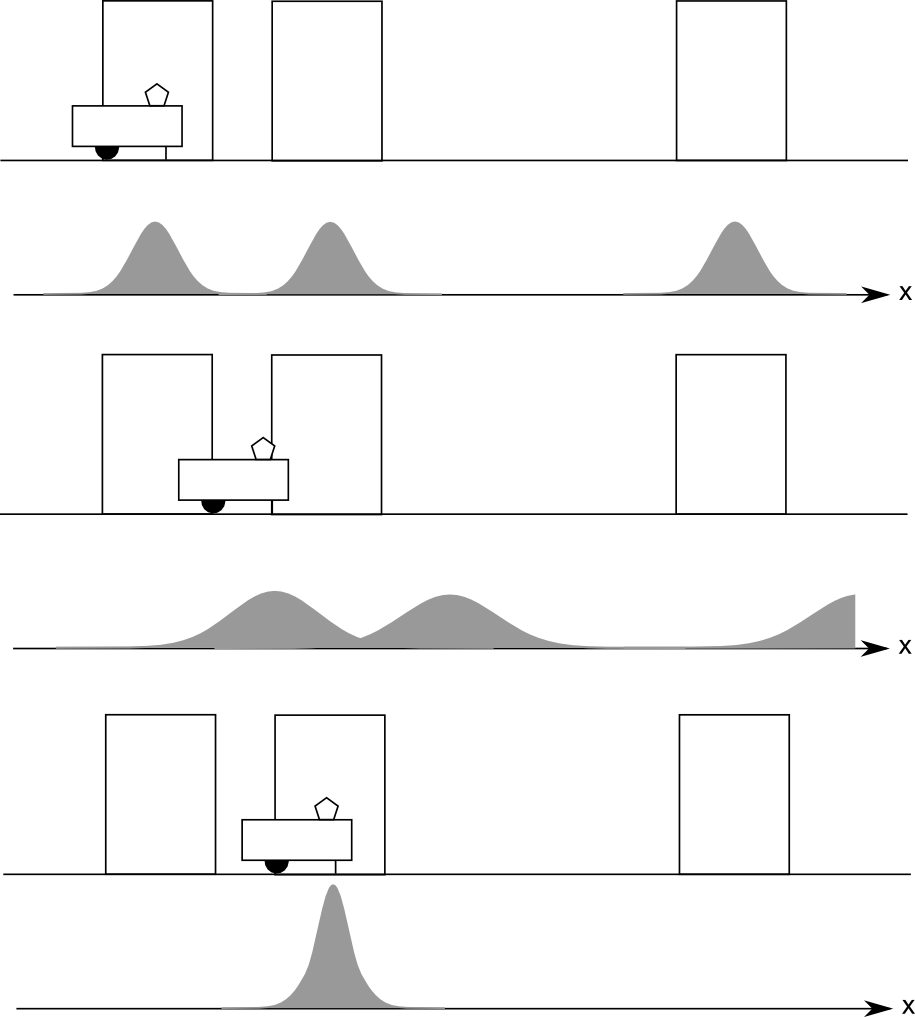
\includegraphics[width=\textwidth]{figs/three_door_example}
	\caption{A robot localizing itself using a ``door detector'' in a known map. Top: Upon encountering a door, the robot can be in front of any of the three doors. Middle: When driving to the right, the Gaussian distributions representing its location also shift to the right and widen, representing growing uncertainty. Bottom: After detecting the second door, the robot can discard hypotheses that are not in front of the door and gains certainty on its location. }
	\label{fig:three_door_example}
\end{figure}

\section{Markov Localization}\label{sec:markovloc}
Calculating the probability to be at a certain location given the likelihood of certain observations is nothing else as a conditional probability. There is a formal way to describe such situations: Bayes' Rule (Section \ref{sec:bayesrule})\index{Bayes' rule}:
\begin{equation}
P(A|B)=\frac{P(A)P(B|A)}{P(B)}
\end{equation}
\subsection{Perception Update}
How does this map into a Localization framework? Lets assume, event $A$ is equivalent to be at a specific location $loc$. Lets also assume that event $B$ corresponds to the event to see a particular feature $feat$. We can now rewrite Bayes' rule to

\begin{equation}
P(loc|feat)=\frac{P(loc)P(feat|loc)}{P(feat)}
\end{equation}

Rephrasing Bayes' rule in this way, we can calculate the probability to be at location $loc$, given that we see feature $feat$. This is known as \emph{Perception Update}\index{Perception Update (Markov Localization)}. For example, $loc$ could correspond to door 1, 2 or 3, and $feat$ could be the event of sensing a door. What do we need to know to make use of this equation?
\begin{enumerate}
\item We need to know the prior probability to be at location loc $P(loc)$
\item We need to know the probability to see the feature at this location $P(feat|loc)$
\item We need the probability to encounter the feature feat $P(feat)$
\end{enumerate}
Lets start with (3), which might be the most confusing part of information we need to collect. The answer is simple, no matter what $P(feat)$ is, it will cancel out as the probability to be at any of the possible locations has to sum up to 1. (A simpler, although less accurate, explanation would be that the probability to sense a feature is constant and therefore does not matter.)

The prior probability to be at location  $loc$, $P(loc)$, is called the \index{Belief Model} \emph{belief model}. In the case of the 3-door example, it is the value of the Gaussian distribution underneath the door corresponding to $loc$. 

Finally, we need to know the probability to see the feature $feat$ at location $loc$ $P(feat|loc)$. If your sensor were perfect, this probability is simply 1 if the feature exists at this location, or 0 if the feature cannot be observed at this location. If your sensor is not perfect, $P(feat|loc)$ corresponds to the likelihood for the sensor to see the feature if it exists.

The final missing piece is how to best represent possible locations. In the graphical example in Figure \ref{fig:three_door_example} we assumed Gaussian distributions for each possible location. Alternatively, we can also discretize the world into a grid and calculate the likelihood of the robot to be in any of its cells. In our 3-door world, it might make sense to choose grid cells that have just the width of a door.

\subsection{Action Update}
One of the assumptions in the above thought experiment was that we know with certainty that the robot moved right. We will now more formally study how to treat uncertainty from motion. Recall, that odometry input is just another sensor that we assume to have a Gaussian distribution; if our odometer tells us that the robot traveled a meter, it could have traveled a  little less or a little more, with decreasing likelihood. We can therefore calculate the posterior probability of the robot moving from a position $loc'$ to $loc$ given its odometer input $odo$:

\begin{equation}
P(loc'->loc|odo)=P(loc'->loc)P(odo|loc'->loc)/P(odo)
\end{equation}

This is again Bayes' rule. The unconditional probability $P(loc'->loc)$ is the prior probability for the robot to have been at location $loc'$. The term $ P(odo|loc'->loc)$ corresponds to the probability to get odometer reading $odo$ after traveling from a position $loc'$ to $loc$. If getting a reading of the amount $odo$ is reasonable for the distance from $loc'$ to $loc$ this probability is high. If its unreasonable, for example if the distance is much larger than the robot could possibly ever have driven, this probability should be very low. 

As the robot's location is uncertain, the real challenge is now that the robot could have potentially been everywhere to start with. We therefore have to calculate the posterior probability $P(loc|odo)$ for all possible positions $loc'$. This can be accomplished by summing over all possible locations:
\begin{equation}
P(loc|odo)=\sum_{loc'}P(loc'->loc)P(odo|loc'->loc)
\end{equation}
In other words, the law of total probability requires us to consider all possible locations the robot could have ever been at. This step is known as \emph{Action Update}\index{Action Update (Markov Localization)}. In practice we don't need to calculate this for all possible locations, but only those that are technically feasible given the maximum speed of the robot. We note also that the sum notation technically corresponds to a convolution (Section \ref{sec:convolution}) of the probability distribution of the robot's location in the environment with the robots odometry error probability distribution.

\subsection{Summary and Examples}
We have now learned two methods to update the belief distribution of where the robot could be in the environment. First, a robot can use external landmarks to update its position. This is known as \emph{perception update} in  and relies on exterioception. Second, a robot can observe its internal sensors. This is known as \emph{action update} and relies on proprioception. The combination of action and perception updates is known as \emph{Markov Localization}\index{Markov Localization}. You can think about the action update to increase the uncertainty of the robot's position and the perception update to shrink it. (You can also think about the action update as a discrete version of the error propagation model.) Also here we are using the robotics kinematic model and the noise model of your odometer to calculate $ P(odo|loc'->loc)$.

\paragraph{Example 1: Topological Map}
This example describes one of the first successful real robot systems that employed Markov Localization in an office environment. The experiment is described in more detail in a 1994 article of AI Magazine. The office environment consisted of two rooms and a corridor that can be modeled by a topological map\index{Topological Map} (Figure \ref{fig:dervish_example}). In a topological map, areas that the robot can be in are modeled as vertices, and navigable connections between them are modeled as edges of a graph. The location of the robot can now be represented as a probability distribution over the vertices of  this graph.

\begin{figure}
	\centering
		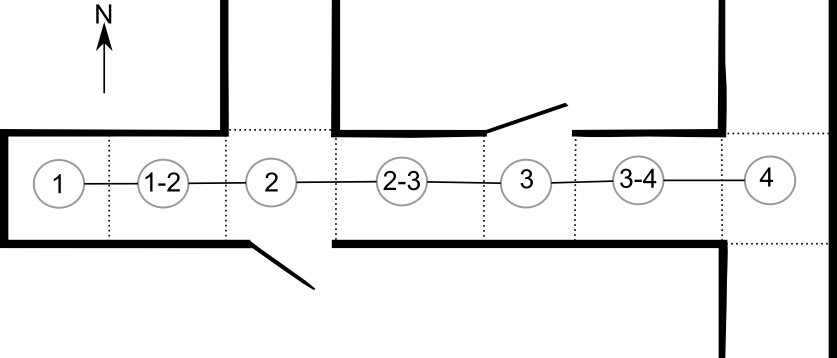
\includegraphics[width=\textwidth]{figs/dervish_example}
	\caption{An office environment consisting of two rooms connected by a hallway. A topological map is super-imposed.}
	\label{fig:dervish_example}
\end{figure}

The robot has the following sensing abilities:
\begin{itemize}
\item It can detect a wall to its left or right.
\item It can detect an open door to its left or right.
\item It can detect a closed door to its left or right.
\item It can detect whether it is an open hallway.
\end{itemize}

Unfortunately, the robot's sensors are not at all reliable. The researchers have experimentally found the probabilities to obtain a certain sensor response for specific physical positions using their robot in their environment. These values are provided in Table \ref{tab:dervish_example}. 

\begin{table}
\footnotesize
\begin{tabular}{lccccc}
 	& Wall	& Closed dr & Open dr	& Open hwy & Foyer\\
\hline
Nothing detected	& 70\%	& 40\%&	5\%	& 0.1\% & 30\%\\
Closed door detected & 30\% &	60\%& 0\% &0\%	& 5\%\\
Open door detected & 0\%	& 0\%&	90\% & 10\% & 15\%\\
Open hallway detected & 0\% &	 0\%&	0.1\% & 90\% &50\%\\
\hline
\end{tabular}
\normalsize
\caption{Conditional probabilities of the Dervish robot detecting certain features in the Stanford laboratory.\label{tab:dervish_example}}
\end{table}

For example, the success rate to detect a closed door is only 60\%, whereas a foyer looks like an open door in 15\% of the trials. This data corresponds to the conditional probability to detect a certain feature given a certain location.

Consider now the following initial belief state distribution: $p(1-2)=0.8$ and $p(2-3)=0.2$. Here, $1-2$ etc.\ refers to the position on the topological map in Figure \ref{fig:dervish_example}. You know that the robot faces east with certainty. The robot now drives for a while until it reports ``open hallway on its left and open door on its right''. This actually corresponds to location 2, but the robot can in fact be anywhere. For example there is a 10\% chance that the open door is in fact an open hallway, i.e.\ the robot is really at position 4. How can we calculate the new probability distribution of the robot's location? Here are the possible trajectories that could happen:

The robot could move from $2-3$ to $3$, $3-4$ and finally $4$. We have chosen this sequence as the probability to detect an open door on its right is zero for $3$ and $3-4$, which leaves position $4$ as the only option if the robot has started at $2-3$. In order for this hypothesis to be true, the following events need to have happened, their probabilities are given in parentheses:
\begin{enumerate}
\item The robot must have started at $2-3$ (20\%)
\item Not have seen the open door at the left of $3$ (5\%) and not have seen the wall at the right (70\%)
\item Not have seen the wall to its left (70\%) and not have seen the wall to its right (70\%) at node $3-4$
\item Correctly identify the open hallway to its left (90\%) and mistake the open hallway to its right for an open door (10\%)
\end{enumerate}
Together, the likelihood that the robot got from position $2-3$ to position $4$ is therefore given by $0.2*0.05*0.7*0.7*0.7*0.9*0.1=0.03\%$, that is very unlikely.


The robot could also move from $1-2$ to $2$, $2-3$, $3$, $3-4$ or $4$. We can evaluate these hypotheses in a similar way:
\begin{itemize}
\item The chance that it correctly detects the open hallway and door at position $2$ is $0.9*0.9$, so the chance to be at position $2$ is
$0.8*0.9*0.9=64\%$.
\item The chance to have seen an open door instead of a wall at $2-3$, $3$, and $3-4$ is zero, so the robot cannot have ended up at these positions.
\item In order to reach position $4$, the robot must not have seen the hallway on its left and the open door to its right when passing position $2$. The probability for this is $0.001*0.05$. The robot must then have detected nothing at $2-3$ ($0.7*0.7$), nothing at $3$ ($0.05*0.7$), nothing at $3-4$ ($0.7*0.7$), and finally mistaken the hallway on its right for an open door at position $4$ ($0.9*0.1$). Multiplied together, this outcome is very unlikely.
\end{itemize}

Given this information, we can now calculate the posterior probability to be at a certain location on the topological map by adding up the probabilities for every possible path to get there. 

\paragraph{Example 2: Grid-based Markov Localization}

\begin{figure}
	\centering
		\includegraphics[width=\textwidth]{figs/markov_grid_example}
	\caption{Markov localization on a grid. The left colum shows the likelihood to be in a specific cell as grey value (dark colors correspond to high likelihoods). The right column shows the actual robot location. Arrows indicate previous motion. Initially, the position of the robot is unknown, but recorded upwards motion makes positions at the top of the map more likely. After the robot has encountered a wall, positions away from walls become unlikely. After rightwards and down motions, the possible positions have shrunk to a small area.}
	\label{fig:markov_grid_example}
\end{figure}

Instead of using a coarse topological map, we can also model the environment as a fine-grained grid. Each cell is marked with a probability corresponding to the likelihood of the robot being at this exact location (Figure \ref{fig:markov_grid_example}). We assume that the robot is able to detect walls with some certainty. The images in the right column show the actual location of the robot. Initially, the robot does not see a wall and therefore could be almost anywhere. The robot now moves northwards. The action update now propagates the probability of the robot being somewhere upwards. As soon as the robot encounters the wall, the perception update bumps up the likelihood to be anywhere near a wall. As there is some uncertainty associated with the wall detector, the robot cannot only be directly at the wall, but anywhere --- with decreasing probability --- close by. As the action update involved continuous motion to the north, the likelihood to be close to the south wall is almost zero. The robot then performs a right turn and travels along the wall in clockwise direction. As soon as it hits the east wall, it is almost certain about its position, which then again decreases.

\section{Particle Filter}
Although grid-based Markov Localization can provide compelling results, it can be computationally very expensive, in particular when the environment is large and the resolution of the grid is small. This is in part due to the fact that we need to carry the probability to be at a certain location forward for every cell on the grid, regardless of how small this probability is. An elegant solution to this problem is the particle filter. It works as follows:
\begin{enumerate}
\item Represent the robots position by N particles that are randomly distributed around its estimated initial position. For this, we can either use one or more Gaussian distributions around the initial estimate(s) of where the robot is, or choose an uniform distribution (Figure \ref{fig:particlefilter_example}).
\item Every time the robot moves, we will move each particle in the exact same way, but add noise to each movement much like we would expect it the real robot to exhibit. Without a perception update, the particles will spread apart farther and farther.
\item Upon a perception event, we evaluate every single particle using our sensor model. What would the likelihood be to have a perception event such as we observed at this location? We can then use Bayes' rule to update each particles position.
\item Once in a while or during perception events that render certain particles infeasible, particles that have a too low probability can be deleted, while those with the highest probability can be replicated.
\end{enumerate}

\begin{figure}
	\centering
		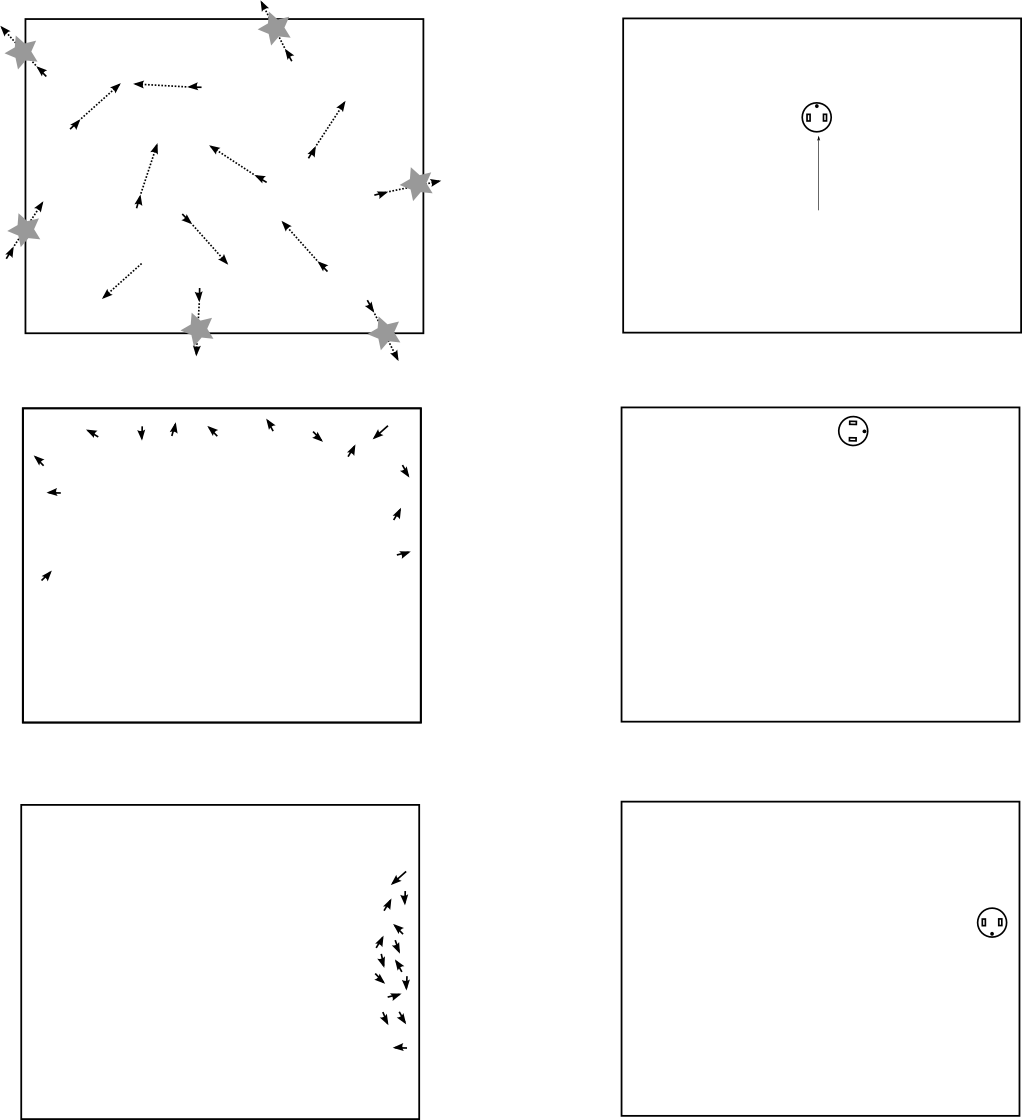
\includegraphics[width=\textwidth]{figs/particlefilter_example}
	\caption{Particle filter example. Possible positions and orientations of the robot are initially uniformly distributed. Particles move based on the robot's motion model. Particles that would require the robot to move through a wall in absence of a wall perception event are deleted (stars). After a perception event, particles too far of a wall become unlikely and their positions are resampled in the vicinity of a wall. Eventually, the particle filter converges.}
	\label{fig:particlefilter_example}
\end{figure}

\section{The Kalman Filter}
The location of a robot is subject to uncertainty due to wheel-slip and encoder noise. We learned in the past how the variance in position can be derived from the variance of the robot's drive train using the error propagation law and the forward kinematics of the robot. One can see that this error is continuously increasing unless the robot has additional observations, e.g., of a static object with known location. This update can be formally done using Bayes' rule, which relates the likelihood to be at a certain position given that the robot sees a certain feature to the likelihood to see this feature at the hypothetical location. For example, a robot that drives towards a wall will become less and less certain of its position (action update) until it encounters the wall (perception update). It can then use its sensor model that relates its observation with possible positions. Its real location must be therefore somewhere between its original belief and where the sensor tells it to be. Bayes' rule allows us to perform this location for discrete locations and discrete sensor error distributions. This is inconvenient as we are used to represent our robot's position with a 2D Gaussian distribution. Also, it seems much easier to just change the mean and variances of this Gaussian instead of updating hundreds of variables. The goals of this section are
\begin{itemize}
\item to introduce a technique known as the Kalman filter to perform action and perception updates exclusively using Gaussian distributions.
\item to formally introduce the notion of a feature map.
\item to develop an example that puts everything we learned so far together: forward kinematics, error propagation and feature estimation.
\end{itemize}

\subsection{Probabilistic Map based localization}
In order to localize a robot using a map, we need to perform the following steps
\begin{enumerate}
\item Calculate an estimate of our new position using the forward kinematics and knowledge of the wheel-speeds that we sent to the robot until the robot encounters some uniquely identifiable feature.
\item Calculate the relative position of the feature (a wall, a landmark or beacon) to the robot.
\item Use knowledge of where the feature is located in global coordinates to predict what the robot should see.
\item Calculate the difference between what the robot actually sees and what it believes it should see.
\item Use the result from (4) to update its belief by weighing each observation with its variance.
\end{enumerate}

Steps 1-2 are based on the lectures on ``Forward Kinematics'' and ``Line detection''. Step 3 uses again simple forward kinematics to calculate the position of a feature stored in global coordinates in a map in robot coordinates. Step 4 is a simple subtraction of what the sensor sees and what the map says. Step 5 introduces the Kalman filter. Its derivation is involved, but its intuition is simple: why just averaging between where I think I am and what my sensors tell me, if my sensors are much more reliable and should carry much higher weight?

\subsection{Optimal Sensor Fusion}
The Kalman filter is an optimal way to fuse observations that follow a Gaussian distribution. The Kalman filter has an update and a prediction step. The update step uses a dynamical model of the system (such as the forward kinematics of your robot) and the prediction step uses a sensor model (such as the error distribution calibrated from its sensors). The Kalman filter does not only update the state of the system (the robot's position) but also its variance. For this, it requires knowledge of all the variances involved in the system (e.g., wheel-slip and sensor error) and uses them to weigh each measurement accordingly. Before providing the equations for the Kalman filter, we will make use a simple example that explains what ``optimal'' means in this context.

 Let $ \hat{q_1}$ and $ \hat{q_2}$ be two different estimates of a random variable and $ \sigma^2_1$ and $ \sigma^2_2$ their variances, respectively. Let $ q$ be the true value. This could be the robot's position, e.g. The observations have different variances when they are obtained by  different means, say using odometry for $ \hat{q_1}$ and by using the location of a known feature for $ \hat{q_2}$. We can now define the weighted mean-square error
 \begin{equation}
S=\displaystyle\sum_{i=1}^{n}\frac{1}{\sigma_i} (q-\hat{q_i})^2
\end{equation}
that is, $ S$ is the sum of the errors of each observation $ \hat{q_i}$ weighted by its standard deviation $ \sigma_i$. Each error is weighted  with its standard deviation to put more emphasis on observations whose standard deviation is low. Minimizing  $S$ for $n=2$ yields the following optimal expression for $q$:
\begin{equation}
q=\frac{\hat{q_1}\sigma_2^2}{\sigma_1^2+\sigma_2^2}+\frac{\hat{q_2}\sigma_1^2}{\sigma_1^2+\sigma_2^2}
\end{equation}
or, equivalently, 
\begin{equation}
q=\hat{q_1}+\frac{\sigma_1^2}{\sigma_1^2+\sigma_2^2}(\hat{q_2}-\hat{q_1})\label{eq:optimalfusion}
\end{equation}

We have now derived an expression for fusing two observations with different errors that provably minimizes the error between our estimate and the real value. As $q$ is a linear combination of two random variables (Section \ref{sec:lcombrandom}, the new variance is given by
\begin{equation}
\sigma^2=\frac{1}{\frac{1}{\sigma_1^2}+\frac{1}{\sigma_2^2}}
\end{equation}
Interestingly, the resulting variance is smaller than both $\sigma_1$ and $\sigma_2$, that is, adding additional observation always helps  reducing accuracy instead of introducing more uncertainty. 

\subsection{Integrating prediction and update: The Kalman Filter}
Although we have introduced the problem above as fusing two observations of the same quantity and weighing them by their variance, we can also interpret the equation above as an update step that calculates a new estimate of an observation based on its old estimate and a measurement. Remember step (4) from above: $ \hat{q_2}-\hat{q_1}$ is nothing else as the difference between what the robot actually sees and what it thinks it should see. This term  is known as innovation in Kalman lingo. We can now 
rewrite (\ref{eq:optimalfusion}) from above into
\begin{equation}
\hat{x}_{k+1}=\hat{x}_k+K_{k+1}\tilde{y}_{k+1}
\end{equation}
Here, $ \hat{x}_k$ is the state we are interested in at time $ k$, $ K_{k+1}=\frac{\sigma_1^2}{\sigma_1^2+\sigma_2^2}$ the Kalman gain, and $ \tilde{y}_{k+1}=\hat{q_2}-\hat{q_1}$  the innovation. Unfortunately, there are few systems that allow us to directly measure the information we are interested in. Rather, we obtain a sensor measurement $ z_k$ that we need to convert into our state somehow. You can think about this the other way round too and predict your measurement $ z_k$ from your state $ x_k$. This is done using the observation model $ H_k$, so that
\begin{equation}
\tilde{y}_{k}=z_k-H_k x_k
\end{equation}
In our example $ H_k$ was just the identity matrix; in a robot position estimation problem $ H_k$ is a function that would predict how a robot would see a certain feature. As you can see, all the weighing based on variances is done in the Kalman gain $ K$.
The perception update step shown above, also known as prediction step is only half of what the Kalman filter does. The first step is the update step, which corresponds to the action update we already know. In fact, the variance update in the Kalman filter is exactly the same as we learned during error propagation. Before going into any more details on the Kalman filter, it is time for a brief disclaimer: the Kalman filter only works for linear systems. Forward kinematics of even the simplest robots are mostly non-linear, and so are observation models that relate sensor observations and the robot position. Non-linear systems can be dealt with the Extended Kalman Filter.

\section{Extended Kalman Filter}\label{sec:EKF}
In the extended Kalman filter, the state transition and observation models need not be linear functions of the state but may instead be differentiable functions. The action update step looks as follows:
\begin{equation}
\hat{\boldsymbol{x}}_{k'|k-1} = f(\hat{\boldsymbol{x}}_{k-1|k-1}, \boldsymbol{u}_{k-1})
\end{equation}
Here $ f()$ is a function of the old state $ \boldsymbol{x}_{k-1}$ and control input $ \boldsymbol{u}_{k-1}$. This is nothing else as the odometry update we are used to, where $ f()$ is a function describing the forward kinematics of the robot, $ \boldsymbol{x}_k$ its position and $ \boldsymbol{u}_k$ the wheel-speed we set.

We can also calculate the covariance matrix of the robot position

\begin{equation}
\boldsymbol{P}_{k'|k-1} = \nabla_{x,y,\theta}f \boldsymbol{P}_{k-1|k-1}\nabla_{x,y,\theta}f^T + \nabla_{\Delta_{r,l}}f\boldsymbol{Q}_{k-1}\nabla_{\Delta_{r,l}}f
\end{equation}

This is nothing else as the error propagation law applied to the odometry of the robot with $ \boldsymbol{Q}_k$ the covariance matrix of the wheel-slip and the Jacobian matrices of the forward kinematic equations $ f()$ with respect to the robot's position (indicated by the index $ x,y,\theta$) and with respect to the wheel-slip of the left and right wheel.

The perception update (or prediction) step looks as follows:

\begin{eqnarray}{ccc}
\hat{\boldsymbol{x}}_{k|k'} &=& \hat{\boldsymbol{x}}_{k'|k-1} + \boldsymbol{K}_{k'}\tilde{\boldsymbol{y}}_{k'}\\
\boldsymbol{P}_{k|k'} &=& (I - \boldsymbol{K}_{k'} {\boldsymbol{H}_{k'}}) \boldsymbol{P}_{k'|k-1}
\end{eqnarray}

At this point the indices $ k$ should start making sense. We are calculating everything twice: once we update from $ k-1$ to an intermediate result $ k'$ during the action update, and obtain the final result after the perception update where we go from $ k'$ to $ k$.

We need to calculate three additional variables:
\begin{enumerate}
\item The innovation $ \tilde{\boldsymbol{y}}_{k}=\boldsymbol{z}_{k}-h(\hat{\boldsymbol{x}}_{k|k-1})$
\item The covariance of the innovation $\boldsymbol{S}_{k}={\boldsymbol{H}_{k}}\boldsymbol{P}_{k|k-1}{\boldsymbol{H}_{k}^\top}+\boldsymbol{R}_{k}$
\item The (near-optimal)  Kalman gain $ \boldsymbol{K}_{k}=\boldsymbol{P}_{k|k-1}{\boldsymbol{H}_{k}^\top}\boldsymbol{S}_{k}^{-1}$
\end{enumerate}
Here $ h()$ is the observation model and $ \boldsymbol{H}$ its Jacobian. How these equations are derived is involved (and is one of the fundamental results in control theory), but the idea is the same as introduced above: we wish to minimize the error of the prediction.

\subsection{Odometry using the Kalman Filter}
We will show how a mobile robot equipped with a laser scanner can correct its position estimate by relying on unreliable odometry, unreliable sensing, but a correct map, in an optimal way.
Whereas the update step is equivalent to forward kinematics and error propagation we have seen before, the observation model and the ``innovation'' require additional steps to perform odometry. 

\paragraph{1.Prediction Update}
We assume for now that the reader is familiar with calculating $ \hat{\boldsymbol{x}}_{k'|k-1}=f(x,y,\theta)^T$ and its variance $ \boldsymbol{P}_{k'|k-1}$. Here, $ \boldsymbol{Q}_{k-1}$, the covariance matrix of the wheel-slip error,  is given by
\begin{equation}
\boldsymbol{Q}_{k-1}=\left[\begin{array}{cc}k_r|\Delta s_r & 0\\0 & k_l|\Delta s_l|\end{array}\right]
\end{equation}
where $ \Delta s$ is the wheel movement of the left and right wheel and $ k$ are constants. See also the odometry lab for detailed derivations of these calculations and how to estimate $ k_r$ and $ k_l$.  The state vector $ \boldsymbol{\hat{x}_{k'|k-1}}$ is a 3x1 vector, the covariance matrix $ \boldsymbol{P_{k'|k-1}}$ is a 3x3 matrix, and $ \nabla_{\Delta_{r,l}}$ that is used during error propagation is a 3x2 matrix. See the error propagation lecture for details on how to calculate $ \nabla_{\Delta_{r,l}}$.

\paragraph{2. Observation}
Let us now assume that we can detect line features $ \boldsymbol{z}_{k,i}=(\alpha_i,r_i)^T$, where $ \alpha$ and $ r$ are the angle and distance of the line from the coordinate system of the robot. These line features are subject to variances $ \sigma_{\alpha,i}$ and $ \sigma_{r,i}$, which make up the diagonal of $ \boldsymbol{R}_{k}$. See the line detection lecture for a derivation of how angle and distance as well as their variance can be calculated from a laser scanner. The observation is a 2x1 matrix.

\paragraph{3. Measurement Prediction}
We assume that we can uniquely identify the lines we are seeing and retrieve their real position from a map. This is much easier for unique features, but can be done also for lines by assuming that our error is small enough and we therefore can search through our map and pick the closest lines. As features are stored in global coordinates, we need to transpose them into how the robot would see them. In practice this is nothing but a list of lines, each with an angle and a distance, but this time with respect to the origin of the global coordinate system. Transposing them into robot coordinates is straightforward. With  $ \hat{\boldsymbol{x}}_{k}=(x_{k},y_{k},\theta_k)^T$ and $ m_i=(\alpha_i,r_i)$ the corresponding entry from the map, we can write

\begin{equation} h(\hat{\boldsymbol{x}}_{k|k-1})=\left[\begin{array}{c}\alpha_{k,i}\\r_{k,i}\end{array}\right]=h(\boldsymbol{x},m_i)=\left[\begin{array}{c}\alpha_i-\theta\\r_i-(x cos(\alpha_i)+y sin(\alpha_i)\end{array}\right]
\end{equation}

and calculate its Jacobian $ \boldsymbol{H}_{k}$ as the partial derivatives of $ \alpha$ to $ x,y,\theta$ in the first row, and the partial derivatives of $ r$ in the second. How to calculate $ h()$ to predict the radius at which the robot should see the feature with radius $ r_i$ from the map is illustrated in the figure below.


\begin{framed}
Example on how to predict the distance to a feature the robot would see given its estimated position and its known location from a map.
\end{framed}

\paragraph{4. Matching}
We are now equipped with a measurement $ \boldsymbol{z}_k$ and a prediction $ h(\hat{\boldsymbol{x}}_{k|k-1})$ based on all features stored in our map. We can now calculate the innovation
\begin{equation}
\tilde{\boldsymbol{y}}_{k}=\boldsymbol{z}_{k}-h(\hat{\boldsymbol{x}}_{k|k-1})
\end{equation}

which is simple the difference between each feature that we can see and those that we predict from the map. The innovation is again a 2x1 matrix.

\paragraph{5. Estimation}
We now have all the ingredients to perform the perception update step of the Kalman filter:

\begin{eqnarray}
\hat{\boldsymbol{x}}_{k|k'} &=& \hat{\boldsymbol{x}}_{k'|k-1} + \boldsymbol{K}_{k'}\tilde{\boldsymbol{y}}_{k'}\\
\boldsymbol{P}_{k|k'} &=& (I - \boldsymbol{K}_{k'} {\boldsymbol{H}_{k'}}) \boldsymbol{P}_{k'|k-1}
\end{eqnarray}

It will provide us with an update of our position that fuses our odometry input and information  that we can extract from features in the environment in a way that takes into account their variances. That is, if the variance of your previous position is high (because you have no idea where you are), but the variance of your measurement is low (maybe from a GPS or a symbol on the Ratslife wall), the Kalman filter will put more emphasis on your sensor. If your sensors are poor (maybe because you cannot tell different lines/walls apart), more emphasis will be on the odometry.

As the state vector is a 3x1 vector and the innovation a 2x1 matrix, the Kalman gain must be a 3x2 matrix. This can also be seen when looking at the covariance matrix that must come out as a 3x3 matrix, and knowing that the Jacobian of the observation function is a 2x3 matrix. We can now calculate the covariance of the innovation and the Kalman gain using

\begin{eqnarray}
\boldsymbol{S}_{k}&=&{\boldsymbol{H}_{k}}\boldsymbol{P}_{k|k-1}{\boldsymbol{H}_{k}^\top}+\boldsymbol{R}_{k}\\
\boldsymbol{K}_{k}&=&\boldsymbol{P}_{k|k-1}{\boldsymbol{H}_{k}^\top}\boldsymbol{S}_{k}^{-1}
\end{eqnarray}

\section*{Take home lessons}
\begin{itemize}
\item If the robot has no additional sensors and its odometry is noisy, error propagation will lead to ever increasing uncertainty of a robots position regardless of using Markov localization or the Kalman filter.
\item Once the robot is able to sense features with known locations, Bayes' rule can be used to update the posterior probability of a possible position. The key insight is that the conditional probability to be at a certain position given a certain observation can be inferred from the likelihood to actually make this observation given a certain position.
\item A complete solution that performs this process for discrete locations is known as Markov Localization. 
\item The Extended Kalman Filter is the optimal way to fuse observations of different random variables that are Gaussian distributed.
It is dervied by minimizing the least-square error between prediction and real value.
\item Possible random variables could be the estimate of your robot position from odometry and observations of static beacons with known location (but uncertain sensing) in the environment.
\item In order to take advantage of the approach, you will need differentiable functions that relate measurements to state variables as well as an estimate of the covariance matrix of your sensors.
\item An approximation that combines benefits of Markov Localization (multiple hypothesis) and the Kalman filter (continuous representation of position estimates) is the Particle filter.
\end{itemize}

\section*{Exercises}\small
\begin{enumerate}
\item Assume that the ceiling is equipped with infra-red markers that the robot can identify with some certainty. Your task is to develop a probabilistic localization scheme, and you would like to calculate the probability $p(marker|reading)$ to be close to a certain marker given a certain sensing reading and information about how the robot has moved.
\begin{enumerate}
\item Derive an expression for $p(marker|reading)$ assuming that you have an estimate of the probability to correctly identify a marker $p(reading|marker)$ and the probability $p(marker)$ of being underneath a specific marker. 
\item Now assume that the likelihood that you are reading a marker correctly is 90\%, that you get a wrong reading is 10\%, and that you do not see a marker when passing right underneath it is 50\%. Consider a narrow corridor that is equipped with 4 markers. You know with certainty that you started from the entry closests to marker 1 and move right in a straight line. The first reading you get is `` Marker 3''. Calculate the probability to be indeed underneath marker 3.
\item Could the robot also possibly be underneath marker 4?
\end{enumerate}
\end{enumerate}\normalsize

% \chapter{Grasping}
\chapter{抓取}

% A robot's end-effector, usually a hand or gripper, is defined by its 6-DOF pose as well as the parameters of its joints such as the opening of the claw or the position of each finger. So far, we have assumed that a robot only needs to plan for a 6-DOF pose that allows the robot to grasp an object from this position. Calculating which position this is and which parameters the end-effector to set is known as grasp planning. This chapter will focus on

机器人的末端执行器,通常是手或夹子,由其6自由度姿态以及其关节的参数(例如爪的打开或每个手指的位置)定义。到目前为止,我们假设一个机器人只需要规划一个6自由度姿态,使机器人能从这个位置抓住一个物体。计算位置以及要设置的末端执行器的参数被称为抓取规划。本章将重点介绍

\begin{enumerate}
% \item What makes a good grasp?
% \item How to find good grasps?
% \item What makes a good grasp?

\item 什么是成功的抓取?
\item 如何找到成功的抓取?
\item 什么决定成功的抓取?
\end{enumerate}

% Think about a three-fingered hand and the problem to grasp a cup. Grasps that are immediately obvious are (1) coming from above and grasping the hull of the cup and (2) wrapping the fingers around the cup. Lets assume that the shape of the cup is cylindric. Then, both of these grasps entirely rely on friction to hold the object. If the normal forces exerted by the fingers are not strong enough, the cup will slip. (It would be possible to re-grasp the object and support it from underneath with one finger if grasped with borderline friction.) A simple model for friction is Coloumb's Friction Law

% It is governed by the equation:

思考用三指的手抓住一个杯子的问题。显而易见的抓取方法有(1)从上方落下,抓住杯子的外壳;(2)将手指绕在杯子周围。假设杯子是圆柱形的。那么,这两种抓取完全依靠摩擦来握住物体。如果手指施加的法向力不够强,那么杯子会滑动。(如果达到边界摩擦力,可以重新抓住物体并用一根手指从下面支撑它。)摩擦力的一个简单的模型是库仑摩擦定律(Coloumb's Friction Law)

它受以下方程的约束:

\begin{equation}
F_\mathrm{t} \leq \mu F_\mathrm{n}
\end{equation}

% where $F_\mathrm{t}$  is the force of friction exerted by each surface on the other and $F_\mathrm{n}$ is the normal force. The force $F_\mathrm{t}$ acts in tangential direction of the normal force applied by, e.g., a finger's tip, where $\mu$ is an empirical coefficient of friction.

其中$F_\mathrm{t}$是一个表面在另一个表面上施加的摩擦力,$F_\mathrm{n}$是法向力。力$F_\mathrm{t}$作用在施加的法向力的切线方向上,例如手指的尖端,其中$\mu$是经验摩擦系数。

% The friction coefficient $\mu$ is low for glass on glass and high for rubber on wood. Coloumb's Fricition law states that the higher the friction coefficient, the more normal force translates into tangential forces that can resist two surfaces from moving against each other. We are therefore interested in designing grippers with high friction coefficients to avoid objects from slipping.

玻璃与玻璃之间的摩擦系数$\mu$低,木材与橡胶之间的摩擦系数高。库仑的摩擦定律指出,摩擦系数越高,法向力越大,越能够抵抗使两个表面相互移动的切向力。因此,我们希望设计具有高摩擦系数的夹具,以避免物体滑动。

% When do objects slip? Lets say we have a fingertip pressing down on a surface in any orientation. There will be a force normal to the surface $F_\mathrm{n}$, which defines the tangential force $F_\mathrm{t}$ in any direction. Sweeping the tangential force around the normal force creates a cone with an opening angle of $2tan^{-1}\mu$. If the net force on the object is not within this cone, the object slips. This becomes more intuitive when thinking about how different values of $\mu$ affect the shape of this cone. If $\mu$ is high, the cone will be relatively flat, letting the object accept forces from many different directions without slipping. If $\mu$ is low, the cone will be relatively narrow, requiring the force to be normal to the object's surface to prevent slippage.

物件何时滑动?让我们假设,我们指尖从任一方向按压在一个表面上。有一个与表面垂直的力$F_\mathrm{n}$,它定义了任何方向上的切向力$F_\mathrm{t}$。围绕法向力旋转切向力产生一个开口角为$2tan^{-1}\mu$的圆锥。如果物体上的净力(Net force)不在此锥体内,物体会滑落。如果考虑$\mu$的不同值如何影响该锥体的形状,这变得更加直观。如果$\mu$高,锥体会相对平坦,让物体可以从许多不同的方向接受力而不会滑动。如果$\mu$低,锥体会相对狭窄,需要与物体表面垂直的力以防止滑动。

% A force applied to a rigid body will exert both a force as well as a torque to the body's center of gravity. This is called a \emph{wrench}\index{Wrench}. If we consider the possible forces that we can apply to a rigid body without having the end-effector slip to form a space (namely the cone described earlier), we can talk about the \emph{grasping wrench space}\index{Grasping wrench space}, which is the corresponding space of all suitable wrenches.

加到刚体的力将对其重心施加力和扭矩。这称为\emph{扭(Wrench)}\index{扭(Wrench)}。如果我们考虑可以施加到刚体而不会使末端执行器滑动形成一个空间(即前面描述的锥体)上的力,那么我们可以讨论\emph{抓取的扭转空间(Grasping wrench space)}\index{抓取的扭转空间(Grasping wrench space)},这是所有合适扳手的对应空间。

% We can also define wrench spaces that suit a specific task, such as picking up an object or opening a door by turning its knob. We can then say that the grasp is good, when the task wrench space is a subset of the grasping wrench space, and will fail otherwise. We can also look at the ratio of forces actually applied to the object and the minimum needed to perform a desired wrench. If this ratio is high, for example, when the robot has to squeeze an object heavily to prevent it from slipping, this grasp is not as good as one, where the ratio is low and all of the force the robot is exerting is actually going into the desired wrench.

我们还可以定义适合特定任务的扭转空间,例如拾取物体或通过旋转门把手打开门。如果任务扭转空间是把手扭转空间的一部分,那么我们可以说抓取是成功的,否则就会失败。我们还可以查看实际施加到物体上的力与达到所需扭转力的最小值的比值。如果这个比例很高(例如,当机器人必须用力地挤压物体以防止它滑落),这种抓取不如比例低、机器人施加的所有力都用到所需的扭转上的抓取好。

% It is usually not possible to find close-form expressions for the grasping wrench space. Instead, one can sample the space of suitable force vectors, e.g., by picking a couple of forces that are on the boundary of the cone's base, and calculate the convex hull over the resulting wrenches.

抓取的扭转空间通常不可能找到近似表达式。相反,我们可以通过在合适的力向量的空间上采样(例如,选择位于锥体底部边界上的力),并计算所得到扭转上的凸包。

% In summary: we can use Coloumb's law of friction to determine the direction of forces that we can apply to a certain contact point without that the object slips. These forces translate into wrenches to the object's center of gravity. A grasp fits a certain task if the wrenches that would fulfill the task can be effectuated without slip. The less force is wasted to overcome slip, the better is the grasp.

总之:我们可以使用库仑的摩擦定律来确定我们可以施加到某个接触点的力的方向,而不会使物体滑动。这些力转化为扭转物体重心上。如果一种抓取能够完成某个任务且没有滑动,那么这种抓取适合这个任务。克服滑动力浪费越少,抓取就越成功。

% \section{How to find good grasps?}
% We are able to determine whether a contact point leads to a good grasp by comparing the grasping wrench spaces that fulfill the task and those that is created by a set of contact points. The question is now how to find good contact points? This is challenging as end-effectors (such as hands) are already quite complicated. A suitable method is therefore to use random sampling, that is bringing the end-effector to random positions, close its fingers around the object, and see what happens when generating wrenches that fulfill the task's requirements.

\section{如何找到成功的抓取?}
通过比较完成任务的抓取的扭转空间和一组接触点创建的扭转空间,我们可以确定一个接触点上能否有成功的抓取。现在的问题是如何找到好的接触点?这是具有挑战性的,因为末端执行器(如手)已经相当复杂。因此,合适的方法是使用随机抽样法,即将末端执行器移到随机位置,将手指围绕物体闭合,并观察在产生满足任务要求的扭转时会发生什么。

% To close the end-effector's fingers around the object requires collision checking. To see what happens, requires dynamic simulation. In short, collision checking routines model an object using a mesh of triangles that can be generated using CAD tools. These triangles are the leafs of a tree that has a coarse bounding object at the top. This coarse bounding object is then split into smaller and smaller elements. Collision checking can now quickly test whether an object collides at all and then recursively refine the exact triangles that collide and finally find the exact points of collision. Dynamic simulation applies Newtonian mechanics to an object (i.e., forces lead to acceleration of a body) and moves the object at very small time-steps. Detecting a collision usually involves moving the objects one step back and then iteratively approaching them until their proximity exceeds a certain treshold.

要闭合环绕物体的末端执行器的手指,需要进行碰撞检测。要看看会发生什么,需要动态模拟。简而言之,碰撞检测例程使用可以用CAD工具生成的三角网格来模拟对象。这些三角就像是在树叶表面有粗糙边界的楞。然后,这个粗大的边界物体被分割成越来越小的三角。碰撞检测现在可以快速测试物体是否碰撞,然后递归细化碰撞的确切三角形,并最终找到确切的碰撞点。动态模拟将牛顿力学应用于物体上(即,力使物体加速),并以非常小的时间步长移动物体。通常碰撞检测将物体后移一步,然后迭代地接近物体,直到其接近度超过一定阈值。




\chapter{Simultaneous Localization and Mapping}\label{chap:slam}
Robots are able to keep track of their position using a model of the noise arising in their drive train and their forward kinematics to propagate this error into a spatial probability density function (Section \ref{sec:errorprop}). The variance of this distribution can shrink as soon as the robot sees uniquely identifiable features with known locations. This can be done for discrete locations using Bayes' rule (Section \ref{sec:markovloc}) and for continuous distributions using the Extended Kalman Filter (Section \ref{sec:ekf}). The key insight here was that every observation will reduce the variance of the robot's position estimate. Here, the Kalman filter performs an optimal fusion of two observations by weighting them with their variance, i.e., unreliable information counts less than reliable one. In the robot localization problem, one of the observations is typically the robot's position estimate whereas the other observation comes from a feature with known location on a map. So far, we have assumed that these locations are known. This chapter will introduce

\begin{itemize}
\item the concept of covariance (or, what all the non-diagonal elements in the covariance matrix are about),
\item how to estimate the robot's location and that of features in the map at the same time (Simultaneous Localization and Mapping or SLAM)
\end{itemize}

\section{Introduction}
The SLAM problem has been considered as the holy grail of mobile robotics for a long time. This lecture will introduce one of the first comprehensive solutions to the problem, which has now be superseded by computationally more efficient versions. We will begin with studying a series of special cases.

\subsection{Special Case I: Single Feature}
Consider a map that has only a single feature. We assume that the robot is able to obtain the relative range and angle of this feature, each with a certain variance. An example of this and how to calculate the variance of an observation based on sensor uncertainty is described in the line fitting example (Section \ref{sec:linefitting}). This feature could be a wall, but also a graphical tag that the robot can uniquely identify. The position of this measurement $m_i=[\alpha_i,r_i]$  in global coordinates is unknown, but can now easily be calculated if an estimate of the robot's position $\boldsymbol{\hat{x}_k}$ is known.  The variance of $ m_i$'s components is now the variance of the robot's position plus the variance of the observation.

Now consider the robot moving closer to the obstacle and obtaining additional observations. Although its uncertainty in position is growing, it can now rely on the feature $m_i$ to reduce the variance of its old position (as long as its known that the feature is not moving). Also, repeated observations of the same feature from different angles might improve the quality of its observation. The robot has therefore a chance to keep its variance very close to that with which it initially observed the feature and stored it into its map. We can actually do this using the EKF framework from Section \ref{sec:EKF}. There, we assumed that features have a known location (no variance), but that the robot's sensing introduces a variance. This variance was propagated into the covariance matrix of the innovation ($ \boldsymbol{S}$). We can now simply add the variance of the estimate of the feature's position to that of the robot's sensing process.

\subsection{Special Case II: Two Features}
Consider now a map that has two features. Visiting one after the other, the robot will be able to store both of them in its map, although with a higher variance for the feature observed last. Although the observations of both features are independent from each other, the relationship between their variances depend on the trajectory of the robot. The differences between these two variances are much lower if the robot connect them in a straight line than when it performs a series of turns between them. In fact, even if the variances of both features are huge (because the robot has already driven for quite a while before first encountering them), but the features are close together, the probability density function over their distance would be very small. The latter can also be understood as the covariance of the two random variables (each consisting of range and angle). In probability theory, the covariance is the measure of how much two variables are changing together. Obviously, the covariance between the locations of two features that are visited immediately after each other by a robot is much higher as those far apart. It should therefore be possible to use the covariance between features to correct estimates of features in retrospect. For example, if the robot returns to the first feature it has observed, it will be able to reduce the variance of its position estimate. As it knows that it has not traveled very far since it observed the last feature, it can then correct this feature's position estimate.

\section{The Covariance Matrix}
When estimating quantities with multiple variables, such as the position of a robot that consists of its x-position, its y-position and its orientation, matrix notation has been a convenient way of writing down equations. For error propagation, we have written the variances of each input variable into the diagonal of a covariance matrix. For example, when using a differential wheel robot, uncertainty in position expressed by $ \sigma_x, \sigma_y$ and $ \sigma_{\theta}$ were grounded in the uncertainty of its left and right wheel. We have entered the variances of the left and right wheel into a 2x2 matrix and obtained a 3x3 matrix that had $ \sigma_x, \sigma_y$ and $ \sigma_{\theta}$ in its diagonal. Here, we set all other entries of the matrix to zero and ignored entries in the resulting matrix that were not in its diagonal. The reason we could actually do this is because uncertainty in the left and right wheel are independent random processes: there is no reason that the left wheel slips, just because the right wheel slips.  Thus the covariance --- the measure on how much two random variables are changing together --- of these is zero. This is not the case for the robot's position: uncertainty in one wheel will affect all output random variables ($ \sigma_x, \sigma_y$ and $ \sigma_{\theta}$) at the same time, which is expressed by their non-zero covariances --- the non-zero entries off the diagonal of the output covariance matrix.

\section{EKF SLAM}\label{sec:ekfslam}
The key idea in EKF SLAM is to extend the state vector from the robot's position to contain the position of all features. Thus, the state
\begin{equation}
\hat{\boldsymbol{x}}_{k'|k-1}=(x,y,\theta)^T
\end{equation}
becomes
\begin{equation}
\hat{\boldsymbol{x}}_{k}=(x,y,\theta,\alpha_1,r_1,\ldots,\alpha_N,r_N)^T
\end{equation}
assuming $ N$ features, which is a $(3+2N) x1$ vector. The action update (or ``prediction update") is identical to that if features are already known; the robot simply updates its position using odometry and updates the variance of it s position using error propagation. The covariance matrix is now a $(3+2N)x(3+2N)$ matrix that initially holds the variances on position and those of each feature in its diagonal.

The interesting things happen during the perception update. Here it is important that only one feature is observed at a time. Thus, if the robot observes multiple features at once, one needs to do multiple, consecutive perception updates. Care needs to be taken that the matrix multiplications work out. In practice you will need to set only those values of the observation vector (a $(3+2N)x1$ vector) that correspond to the feature that you observe. Similar considerations apply to the observation function and its Jacobian.

\section{Graph-based SLAM}
Usually, a robot obtains an initial estimate of where it is using some onboard sensors (odometry, optical flow, etc.) and uses this estimate to localize features (walls, corners, graphical patterns) in the environment. As soon as a robot revisits the same feature twice, it can update the estimate on its location. This is because the variance of an estimate based on two independent measurements will always be smaller than any of the variances of the individual measurements. As consecutive observations are not independent, but rather closely correlated, the refined estimate can then be propagated along the robot's path. This is formalized in EKF-based SLAM. A more intuitive understanding is provided by a spring-mass analogy: each possible pose (mass) is constrained to its neighboring pose by a spring. The higher the uncertainty of the relative transformation between two poses (e.g., obtained using odometry), the weaker the spring. Every time a robot gains confidence on a relative pose, the spring is stiffened instead. Eventually, all poses will be pulled in place. This approach is known as \emph{Graph-based SLAM}\index{Graph-based SLAM}. 

\subsection{SLAM as a Maximum-Likelihood Estimation Problem}
The classical formulation of SLAM describes the problem as maximizing the posterior probability of all points on the robot's trajectory given the odometry input and the observations. Formally,
\begin{equation}
p(x_{1:T},m|z_{1:T},u_{1:T})
\end{equation}
where $ x_{1:T}$ are all discrete positions from time 1 to time $ T$, $ z$ are the observations, and $ u$ are the odometry measurements. This formulation makes heavily use of the temporal structure of the problem. In practice, solving the SLAM problem requires
\begin{enumerate}
\item A motion update model, i.e., the probability $ p(x_t|x_{t-1},u_t)$ to be at location $ x_t$ given an odometry measurement $ u_t$ and being at location $ x_{t-1}$.
\item  A sensor model, i.e., the probability $ p(z_t|x_t,m_t)$ to make observation $ z_t$ given the robot is at location $ x_t$ and the map $ m_t$.
\end{enumerate}
A possible solution to this problem is provided by the Extended Kalman Filter, which maintains a probability density function for the robot pose as well as the positions of all features on the map. Being able to uniquely identify features in the environment is of outmost importance and is known as the data association problem. Like EKF-based SLAM, graph-based SLAM does not solve this problem and will fail if features are confused.

In graph-based SLAM, a robot's trajectory forms the nodes of a graph whose edges are transformations (translation and rotation) that have a variance associated with it. An alternative view is the spring-mass analogy mentioned above. Instead of having each spring wiggle a node into place, graph-based SLAM aims at finding those locations that maximize the joint likelihood of all observations. As such, graph-based SLAM is a \emph{maximum likelihood estimation}\index{Maximum Likelihood Estimation} problem.

Lets revisit the normal distribution:
\begin{equation}
\frac{1}{\sigma\sqrt{2\pi}}e^{\frac{-(x-\mu)^2}{2\sigma^2}}
\end{equation}

It provides the probability for a measurement to have value $ x$ given that this measurement is normal distributed with mean $ \mu$ and variance $ \sigma^2$.  We can now associate such a distribution with every node-to-node transformation, aka constraint. This can be pairs of distance and angle, e.g. In the literature the measurement of a transformation between node i and a node j is denoted $ z_{ij}$. Its expected value is denoted $ \hat{z}_{ij}$. This value is expected for example based on a map of the environment that consists of previous observations.

Formulating a normal distribution of measurements $ z_{ij}$ with mean $ \hat{z}_{ij}$ and a covariance matrix $ \Sigma_{ij}$ (containing all variances of the components of $ z_{ij}$ in its diagonal) is now straightforward. As graph-based SLAM is most often formulated as  information filter, usually the inverse of the covariance matrix (aka information matrix) is used, which we denote by $ \Omega_{ij}=\Sigma_{ij}^{-1}$.

As we are interested in maximizing the joint probability of all measurements $ \prod{z_{ij}}$ over all edge pairings $ ij$ following the maximum likelihood estimation framework, it is customary to express the PDF using the log-likelihood. By taking the natural logarithm on both sides of the PDF expression, the exponential function vanishes and $ ln \prod{z_{ij}}$ becomes $ \sum{ ln z_{ij}}$ or $ \sum{l_{ij}}$, where $ l_{ij}$ is the log-likelihood distribution for $ z_{ij}$.
\begin{equation}
l_{ij} \propto (z_{ij}-\hat{z}_{ij}(x_i,x_j))^T\Omega_{ij}(z_{ij}-\hat{z}_{ij}(x_i,x_j))
\end{equation}

Again, the log-likelihood for observation $ z_{ij}$ is directly derived from the definition of the normal distribution, but using the information matrix instead of the covariance matrix and is ridden of the exponential function by taking the logarithm on both sides.

The optimization problem can now be formulated as
\begin{equation}
x^* = \arg \min_{x}\sum_{<i,j>\in \mathcal{C}}e_{ij}^T\Omega_{ij}e_{ij}
\end{equation}
with $ e_ij(x_i,x_j)=z_{ij}-\hat{z}_{ij}(x_i,xj)$ the error between measurement and expected value. Note that the sum actually needs to be minimized as the individual terms are technically the negative log-likelihood.

\subsection{Numerical Techniques for Graph-based SLAM}
Solving the MLE problem is non-trivial, especially if the number of constraints, i.e., observations that relate one feature to another, provided is large. A classical approach is to linearize the problem at the current configuration and reducing it to a problem of the form $ Ax=b$. The intuition here is to calculate the impact of small changes in the positions of all nodes on all $ e_{ij}$. After performing this motion, linearization and optimization can be  repeated until convergence. 

More recently, more powerful numerical methods have been developed. Instead of solving the MLE, on can employ a stochastic gradient descent algorithm. A gradient descent algorithm is an iterative approach to find the optimum of a function by moving along its gradient. Whereas a gradient descent algorithm would calculate the gradient on a fitness landscape from all available constraints, a stochastic gradient descent picks only a (non-necessarily random) subset. Intuitive examples are fitting a line to a set of $n$ points, but taking only a subset of these points when calculating the next best guess. As gradient descent works iteratively, the hope is that the algorithm takes a large part of the constraints into account. For solving Graph-based SLAM, a stochastic gradient descent algorithm would not take into account all constraints available to the robot, but  iteratively work on one constraint after the other. Here, constraints are observations on the mutual pose of nodes $i$ and $j$. Optimizing these constraints now requires moving both nodes $i$ and $j$ so that the error between where the robot thinks the nodes should be and what it actually sees gets reduced.  As this is a trade-off between multiple, maybe conflicting observations, the result will approximate a Maximum Likelihood estimate.

More specifically, with $ e_ij$ the error between an observation and what the robot expects to see, based on its previous observation and sensor model, one can distribute the error along the entire trajectory between both features that are involved in the constraint. That is, if the constraint involves features $i$ and $j$, not only $i$ and $j$'s pose will be updated but all points inbetween will be moved a tiny bit.

%This approach is cumbersome and quickly gets out of control if a robot is mapping an environment over multiple hours --- leading to millions of nodes in the graph and constraints. To overcome this problem, [Gris07] propose to (1) merge nodes of a graph as it is build up by relying on accurate localization of the robot within the existing map and (2) to chose a different graph representation.

In Graph-based SLAM, edges encode the relative translation and rotation from one node to the other. Thus, altering a relationship between two nodes will automatically propagate to all nodes in the network. This is because the graph is essentially a chain of nodes whose edges consist of odometry measurements. This chain then becomes a graph whenever observations (using any sensor) introduce additional constraints. Whenever such a ``loop-closure'' occurs, the resulting error will be distributed over the entire trajectory that connects the two nodes. This is not always necessary, for example when considering the robot driving a figure-8 pattern. If a loop-closure occurs in one half of the 8, the nodes in the other half of the 8 are probably not involved.

This can be addressed by constructing a  minimum spanning-tree  (MST) of the constraint graph. The MST is constructed by doing a Depth-First Search (DFS) on the constraint graph following odometry constraints. At a loop-closure, i.e., an edge in the graph that imposes a constraint to a previously seen pose, the DFS backtracks to this node and continues from there to construct the spanning tree. Updating all poses affected by this new constraint still requires modifying all nodes along the path between the two features that are involved, but inserting additional constraints is greatly simplified. Whenever a robot observes new relationships between any two nodes, only the nodes on the shortest path between  the two features on the MST need to be updated. %Example graphs illustrating this are shown in Figures 2a and 2b in [Gris07].
\subsection*{Further reading}
\begin{itemize}
\item G. Grisetti, R. Kuemmerle, C. Stachniss and W. Burgard. A Tutorial on Graph-Based SLAM. IEEE Intelligent Transportation Systems Magazine, 2(4):31-43, 2010.

\item E. Olson, J. Leonard and S. Teller. Fast Iterative Alignment of Pose Graphs with Poor Initial Estimates. Proc. of ICRA, pp 2262-2269, Orlando, FL, 2006.

\item G. Grisetti, C. Stachniss, S. Grzonka and W. Burgard. A Tree Parameterization for Efficiently Computing Maximum Likelihood Maps using Gradient Descent. Robotics: Science and Systems (RSS), Atlanta, GA, USA, 2007.
\end{itemize}

\chapter{RGB-D SLAM} 
 Range sensors have emerged as one of the most effective sensors to make robots autonomous. Unlike vision, range data makes the construction of a 3D model of the robot's environment straightforward and the Velodyne sensor, that combines 64 scanning lasers into one package, was key in mastering the DARPA Grand Challenge.  3D range data has become even more important in robotics with the advent of cheap (priced at a tenth than the cheapest 2D laser scanner) RGB-D (color image plus depth) cameras. Point cloud data allows fitting of lines using RANSAC, which can serve as features in EKF-based localization, but can also be used for improving odometry, loop-closure detection, and mapping. The goals of this chapter are
\begin{itemize}
\item introduce the Iterative Closest Point (ICP) algorithm
\item show how ICP can be improved by providing initial guesses via RANSAC
\item show how SIFT features can be used to improve point selection and loop-closure in ICP to achieve RGB-D mapping
\end{itemize}

\section{Converting range data into point cloud data}
Point cloud data can be thought of a 3D matrix that maps a certain volume in 3D space. Each cell in this matrix, also known as \emph{Voxel}\index{Voxel}, corresponds to whether there is an obstacle in this volume or not. Different intensity values could correspond to the uncertainty with which this space is to be known to be an obstacle. An efficient method to turn range information into such an uncertainty 3D map is described in \cite{curless96} and became known as \emph{Truncated Surface Distance Function} (TSDF)\index{Truncated Surface Distance Function (TSDF)}\index{TSDF}, commonly referred to as ``Point cloud''\index{Point cloud}.

\section{The Iterative Closest Point (ICP) algorithm}
The \emph{Iterative Closest Point} (ICP)\index{Iterative Closest Point}\index{ICP} algorithm was presented in the early 1990ies for registration of 3D range data to CAD models of objects. A more in-depth overview of what is described here is given in \cite{rusinkiewicz01}. The key problem can be reduced to find the best transformation that minimizes the distance between two point clouds. This is the case when matching snapshots from a range sensor or matching a range image with a point cloud sampled from a 3D representation of an object.

In robotics, ICP found an application to match scans from 2D laser range scanners. For example, the transformation that minimizes the error between two consecutive snapshots of the environment is proportional to the motion of the robot. This is a hard problem as it is unclear, which points in the two consecutive snapshots are ``pairs", which of the points are outliers (due to noisy sensors), and which points need to be discarded as not all points overlap in both snapshots. Stitching a series of snapshots together theoretically allows to create a 2D map of the environment. This is difficult, however, as the error between every snapshots ---similar to odometry --- accumulates.   The ICP algorithm also works in 3D where it allows to infer the change in 6D pose of a camera and creation of 3D maps. In addition, ICP has proven useful for identifying objects from a database of 3D objects.

Before providing a solution to the mapping problem, we will focus on the ICP algorithm to match 2 consecutive frames. Variants of the ICP algorithm can be broken down into 6 consecutive steps:
\begin{enumerate}
\item Selection of points in one or both meshes or point clouds.
\item Matching/Pairing these points to samples in the other point cloud/mesh.
\item Weighting the corresponding pairs.
\item Rejecting certain pairs.
\item Assigning an error metric based on the point pairs.
\item Minimizing the error metric.
\item Point Selection
\end{enumerate}
Depending on the number of points generated by the range sensor, it might make sense to use only a few selected points to calculate the optimal transformation between two point clouds, and then test this transformation on all points. Depending on the source of the data, it also turns out that some points are more suitable than others as it is easier to identify matches for them. This is the case for RGB-D data, where SIFT features have been used successfully. This is also the case for planar objects with grooves, where sampling should ensure that angles of normal vectors of sampling points are broadly distributed. Which method to use is therefore strongly dependent on the kind of data being used and should be considered for each specific problem.

\subsection{Matching Points}
The key step in ICP is to match one point to its corresponding point.  For example, a laser scanner hits a certain point at a wall with its 67th ray. After the scanner has been moved by 10cm , the closest hit on the wall to this point might have been by the 3rth ray of the laser. Here, it is actually very unlikely that the laser hits the exact same point on the wall twice, therefore introducing a non-zero error even for optimal pairing. Prominent methods are to find the closest point in the other point cloud or to find the intersection of the source points normal with the destination surface (for matching point clouds to meshes). More recently, SIFT has allowed to match points based on their visual appearance. Similarly to sorting through SIFT features, finding the closest matching point can be accelerated by representing the point cloud in a k-d tree.

\subsection{Weighting of Pairs}
As some pairs are better matches than others, weighting them in some smart way might drastically improve the quality of the resulting transformation. One approach is to give more weight to points that have smaller distances from each other. Another approach is to take into account the color of the point (in RGB-D images) or use the distance of their SIFT features (weighting pairs with low distances higher than pairs with high distances). Finally, expected noise can be used to weight pairings. For example, the estimates made by a laser scanner are much more faithful when taken orthogonally to a plane than when taken at a steep angle.

\subsection{Rejecting of Pairs}
A key problem in ICP are outliers either from sensor noise or simply from incomplete overlap between two consecutive range images. A prime approach in dealing with this problem is to reject pairings of which one of the points lies on a boundary of the point cloud as these points are likely to match with points in non-overlapping regions. As a function of the underlying data, it might also make sense to reject pairings with too high of a distance. This is a threshold-based equivalent to distance-based weighting as described above.

\subsection{Error Metric and Minimization Algorithm}
After points have been selected and matched, pairs have been weighted and rejected, the match between two point clouds needs to be expressed by a suitable error metric, which needs then to be minimized. A straightforward approach is to consider the sum of squared distances between each pair. This formulation can often be solved analytically. Let
\begin{eqnarray}
A=\{a_1,\ldots,a_m\}\\
B=\{b_1,\dots,b_n\}
\end{eqnarray}
be point clouds in $ \mathbb{R}^n$. The goal is now to find a vector $ t \in \mathbb{R}^n$ so that an error function $ \phi(A+t,B)$ is minimized. In 6D (translation and rotation), an equivalent notation can be found for a transformation (see forward kinematics). An error function for the squared distance is then given by
\begin{equation}
\phi(A+t,B)=\frac{1}{m}\sum_{a \in A}\|a+t-N_B(a+t)\|^2
\end{equation}
Here $ N_B(a+t)$ is a function that provides the nearest neighbor of $ a$ translated by $ b$ in $ B$.  A key problem now is that the actual value of $t$ affects the outcome of the pairing. What might look like a good match initially often turns out not be the final pairing. A simple numerical approach to this problem is to find $ t$ iteratively.

Initially $t=0$ and nearest neighbors/pairings are established. We can now calculate a $ \delta t$ that optimizes the least-square problem based on this matching using any solver available for the optimization problem (for a least-square solution $ \delta t$ can be obtained analytically by solving for the minimum of the polynomial by setting its derivative to zero). We can then shift all points in $ A$ by $ \delta t$ and start over. That is, we calculate new pairings and derive a new $ \delta t$.  We can continue to do this, until the cost function reaches a local minimum.

Instead of formulating the cost function as a ``point-to-point'' distance, a ``point-to-plane'' has become popular. Here, the cost function consist of the sum of squared distances from each source point to the plane that contains the destination point and is oriented perpendicular to the destination normal. This makes particularly sense when matching a point cloud to a mesh/CAD model of an object. In this case there are no analytical solutions to finding the optimal transformation, but any optimization method such a Levenberg-Marquardt can be used.

\section{RGB-D Mapping}
The ICP algorithm can be used to stitch consecutive range images together to create a 3D map of the environment \cite{henry2010rgb}. Together with RGB information, it is possible to create complete 3D walk throughs of an environment. An example of such a walk through using the method described in \cite{whelan2013robust} is shown in Figure \ref{fig:kintinous}.
A problem with ICP is that errors in each transformation propagate making maps created using this method as odd as maps created by simple odometry. Here, the SLAM algorithm can be used to correct previous errors once a loop closure is detected.


\begin{figure}
\centering
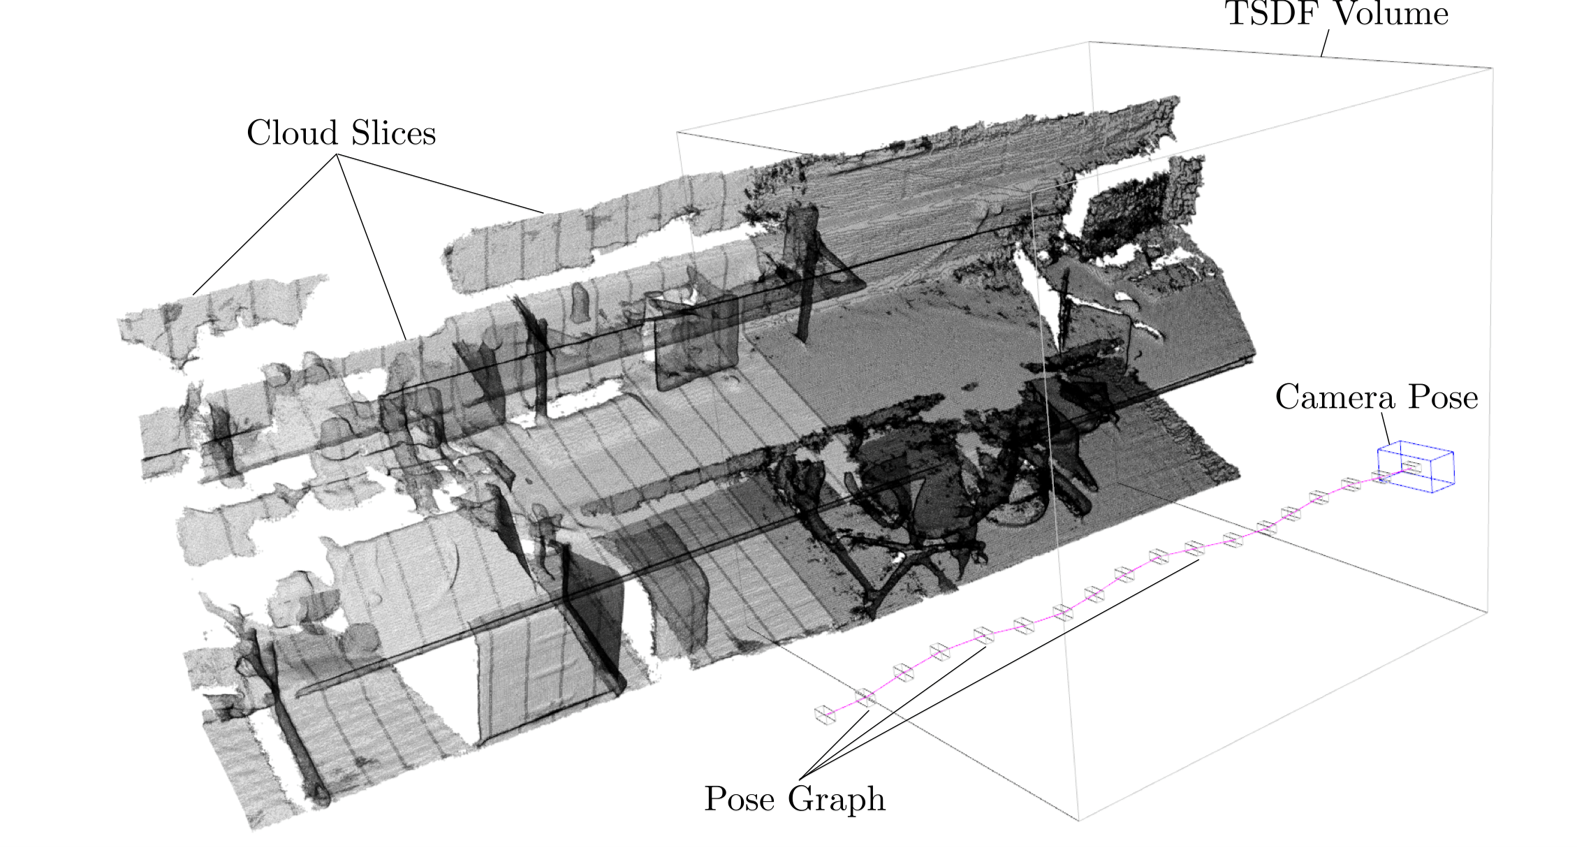
\includegraphics[width=\textwidth]{figs/kintinous}
\caption{Fused point cloud data from a walk trough of an office environment using ``Kintinious''. Picture courtesy of John Leonard.\label{fig:kintinous}}
\end{figure}

The intuition behind SLAM is to consider each transformation between consecutive snapshots as a spring with variable stiffness. Whenever the robot returns to a previously seen location, i.e., a loop-closure has been determined, additional constraints are introduced and the collection of snapshots connected by springs become a mesh. Everytime the robot then re-observes a transformation between any of the snapshots, it can ``stiffen'' the spring connecting the two. As all of the snapshots are connected, this new constraints propagates through the network and literally pull each snapshots in place.

RGB-D Mapping uses a variant of ICP that is enhanced by SIFT features for point selection and matching. Maps are build incrementally. SIFT features, and their spatial relationship, are used for detecting loop closures. Once a loop closure is detected, an additional constraint is added to the pose graph and a SLAM-like optimization algorithm corrects the pose of all previous observations.

As ICP only works when both point clouds are already closely aligned, which might not be the case for a fast moving robot with a relatively noisy sensor (the XBox Kinect has an error of 3cm for a few meters of range vs. millimeters in laser range scanners), RGB-D Mapping uses RANSAC to find an initial transformation. Here, RANSAC works as for line fitting: it keeps guessing possible transformations for 3 pairs of SIFT feature points and then counts the number of inliers when matching the two point clouds, one of which being transformed using the random guess.



\appendix

\chapter{Statistics}\label{chap:statistics}
\section{Random Variables and Probability Distributions}\label{sec:pdfs}
Random variables can describe either discrete variables, such as the result from throwing a dice, or continuous variables such as measuring a distance. In order to learn about the likelihood that a random variable has a certain outcome, we can repeat the experiment many times and record the resulting \emph{random variates}\index{Variate (Random variable)}, that is the actual values of the random variable, and the number of times they occurred. For a perfectly cubic dice we will see that the random variable can hold natural numbers from 1 to 6, that have the same likelihood of 1/6.

The function that describes the probability of a random variable to take certain values is called a \emph{probability distribution}\index{Probability Distribution}.
As the likelihood of all possible random variates in the dice experiment is the same, the dice follows what we call a \emph{uniform distribution}\index{Uniform Distribution}. More accurately, as the outcomes of rolling a dice are discrete numbers, it is actually a discrete uniform distribution. Most random variables are not uniformly distributed, but some variates are more likely than others. For example, when considering a random variable that describes the sum of two simultaneously thrown dice, we can see that the distribution is anything but uniform:

2: 1+1\\
3: 1+2, 2+1\\
4: 1+3, 2+2, 3+1\\
5: 1+4, 2+3, 3+2, 4+1\\
6: 1+5, 2+4, 3+3, 4+2, 5+1\\
7: 1+6, 2+5, 3+4, 4+3, 5+2, 6+1\\
8: 2+6, 3+5, 4+4, 5+3, 6+2\\
9: 3+6, 4+5, 5+4, 6+3\\
10: 4+6, 5+5, 6+4\\
11: 5+6, 6+5\\
12: 6+6\\

As one can see, there are many more possibilities to sum up to a 7 than there are to a 3, e.g. While it is possible to store probability distributions such as this one as a look-up table to predict the outcome of an experiment (or that of a measurement), it is hard to reason about the random process analytically. We therefore aim to describe the probability distributions of random processes that we need to deal with using one of the ``standard'' probability distribution functions (or more accurately probability density function). These functions have been well studied and come with a broad set of tools for their analysis.  Consequently, more often than not we use a well studied probability density function even if the underlying data doesn't fully support its use for the simple reason that we can work its associated mathematical tools.

\subsection{Normal Distribution with different means and variances}
One of the most prominent distributions is the Gaussian or Normal Distribution. The \emph{Normal distribution}\index{Normal Distribution}\index{Gaussian Distribution} is characterized by a \emph{mean} and a \emph{variance}. Here, the mean corresponds to the average value of a random variable (or the peak of the distribution) and the variance is a measure of how broadly variates are spread around the mean (or the width of the distribution).

 The Normal distribution is defined by the following function
 \begin{equation}
f(x)=\frac{1}{\sqrt{2\pi\sigma^2}}e^{-\frac{(x-\mu)^2}{2\sigma^2}}
\end{equation}
where $ \mu$ is the mean and $ \sigma^2$ the variance. ($ \sigma$ on its own is known as the standard deviation.) Then, $ f(x)$ is the probability for a random variable $ X$ to have value $ x$.

\begin{figure}
	\centering
		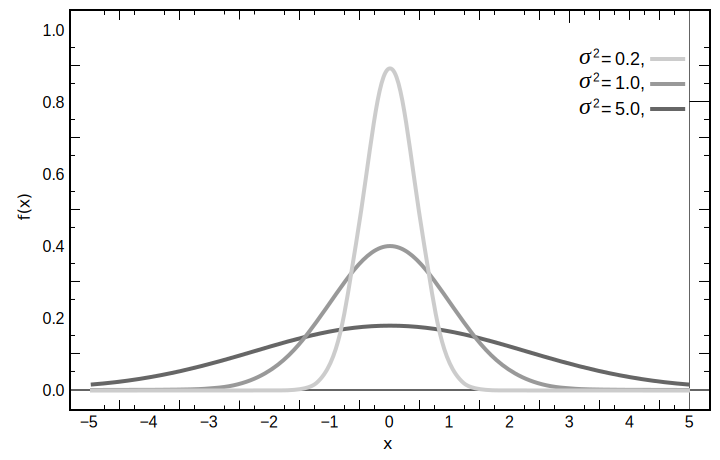
\includegraphics[width=\textwidth]{figs/Normal_Distribution_PDF}
	\caption{Normal distribution for different variances and $\mu=0$.}
	\label{fig:Normal_Distribution_PDF}
\end{figure}

The mean is calculated by
\begin{equation}
\mu=\int_{-\infty}^{\infty}xf(x)dx
\end{equation}
or in other words, each possible value $ x$ is weighted by its likelihood and added up.
\begin{framed}
Exercise: do this for the double dice experiment. Calculate the probability of each outcome from the table above, multiply it with its value and add them all up.
\end{framed}

The variance is calculated as follows
$ \sigma^2=\int_{-\infty}^{\infty}(x-\mu)^2f(x)dx$
or in other words, we calculate the deviation of each random variable from the mean, square it, and weigh it by its likelihood. Although it is tantalizing to perform this calculation also for the double dice experiment, the resulting value is questionable, as the double dice experiment does not follow a Normal distribution. We know this, because we actually enumerated all possible outcomes. For other experiments, such as grades in the classes you are taking, we don't know what the real distribution is.

\subsection{Normal distribution in two dimensions}
The Normal Distribution is not limited to random processes with only one random variable. For example, the X/Y position of a robot in the plane is a random process with two dimensions. In case of a multi-variate distribution with $k$ dimensions, the random variable $ X$ is a k-dimensional vector of random variables, $ \mu$ is a k-dimensional vector of means, and $ \sigma$ gets replaced with $ \Sigma$,  a k-by-k dimensional \emph{covariance matrix}\index{Covariance Matrix} (a matrix that carries the variances of each random variable in its diagonal).

\section{Bayes Rule}\label{sec:bayesrule}
Bayes' Rule relates a conditional probability to its inverse. In other words, if we know the probability of event $A$ to happen given that event $B$ is happening, we can calculate the probability of $B$ to occur given that $A$ is happening. Bayes' rule can be derived from the simple observation that the probability of $A$ and $B$ to happen together ($P(A \cap B)$) is given by $P(A)P(B|A)$ or the probability of $A$ to happen and the probability of $B$ to happen given that $A$ happens. Similarly, we can write
\begin{equation}
P(A \cap B)=P(A)P(B|A)=P(B)P(A|B)
\end{equation}
From this, deriving Bayes' rule is straightforward:
\begin{equation}
P(A|B)=\frac{P(A)P(B|A)}{P(B)}
\end{equation}
In words, if we know the probability that $B$ happens given that $A$ happens, we can calculate that $A$ happens given that $B$ happens. 

\section{Testing Statistical Significance}\label{sec:stattest}
Robotics is an experimental discipline. This means that algorithms and systems you develop need to be validated by real hardware experiments. Doing an experiment to validate your hypothesis is at the core of the scientific method and doing it right is a discipline on its own. The key is to show that your results is not simply a result of chance. In practice, this is impossible to show. Instead, it is possible to express the likelihood that your results have not been obtained by chance. This is known as the statistical significance level. How to calculate the statistical significance level depends on the problem you are studying. This section will introduce three common problems in robotics:

\begin{enumerate}
\item testing whether data is indeed distributed according to a specific distribution
\item testing whether two sets of data are generated from different distributions
\item testing whether true-false experiments are a sequence of luck or not
\end{enumerate}

\subsection{Null Hypothesis on Distributions}
The Null Hypothesis is a term from the statistical significance literature and formally captures your main claim. A statistical test can either reject the Null Hypothesis or fail to reject it. It can never be proven as there will always be a non-zero probability that all your experiments are just a lucky coincidence. The statistical significance level of a Null Hypothesis is known as the p-value.

An import class of Null Hypothesis are on the distribution of data. Consider the following example from Lab 1 (message passing in ROS). Students were asked to experimentally study the time it takes to pass a message from one process to another:

\begin{framed}
Histogram of the time it takes to send a ROS message from one process to another based on 10 trials.
\end{framed}

We observe three peaks in this Histogram. What can we say about message passing times? For example
\begin{itemize}
\item H0: Message passing times follow a Gaussian distribution.
\item H0: Message passing times follow a bi-modal distribution.
\item H0: Message passing times follow a log-normal distribution.
\end{itemize}

The first Null Hypothesis implies that messages take sometimes a little longer and sometimes a little shorter, but have an average and a variance. The second Null Hypothesis implies that usually messages take some low average time, but occasionally are delayed due to the influence of some other process, for example operating system duties. You can now test each of these hypotheses by calculating the parameters of the distribution to expect and calculate the joint probability that each of your measurements are actually drawn from this distribution. You will find, that all of the above hypotheses are almost equally likely. Together, none of your tests will reject your hypothesis. You therefore will need more data:

\begin{framed}
Histogram of message passing times in ROS based on a 1000 trials.
\end{framed}

You can now again calculate parameters for each distribution you suspect. For example, you can calculate the mean and variance of this data and plot the resulting Gaussian distribution. In this example, the Gaussian distribution will have a mean slightly offset to the right of the peak. You can also fit the data to a log-normal distribution. You can now calculate the likelihood for the data actually be drawn from either of the two distributions. You will see that the joint probability (the product of all likelihoods) for all data points is actually much higher than that for any Gaussian distribution or any bimodal distribution that you are able to fit.

Formally, this can be done by following Pearsons $ \chi^2$-Test (read Chi-Squared Test). This test calculates a value that will approximate a $ \chi^2$-distribution from all samples and the likelihood of that sample based on the expected distribution. Plugging the resulting value into the $ \chi^2$-distribution leads to the statistical significance level (or p-value).

The value of the test-statistic is calculated as follows:
\begin{equation}
\chi^2 = \sum_{i=1}^{n} \frac{(O_i - E_i)^2}{E_i}
\end{equation}
where
\begin{itemize}
\item $ \chi^2$ = Pearson's cumulative test statistic, which asymptotically approaches a chi-squared distribution.
\item $ O_i$ = an observed frequency in the data histogram
\item $ E_i$ = an expected (theoretical) frequency, asserted by the null hypothesis, i.e., the distribution you think the data should follow
\item n = the number samples.
\end{itemize}
This example also illustrates how statistical tests can be used to determine if you have enough data. If you don't, you will get very poor p-values.  In practice, it is up to you what likelihood you determine to be significant. Standard significance levels are 10\%, 5\% and 1\%. If you are unsatisfied with your p-values you can collect more data and check, whether your p-value improves.

\subsection{Testing whether two distributions are independent}
Testing whether the data of two experiments are independent is probably the most common statistical test. For example, you might run 10 experiments using algorithm 1 and 10 experiments using algorithm 2. It is up to you to show that the resulting distributions are indeed statistically significantly different. In other words, you need to show that the differences between the algorithm indeed lead to a systematic improvement, and that it was not purely luck that one set of experiments turned out ``better'' than another.

If you have good reasons to believe that your data is normal distributed, there exist a series of simple tests. For example, to test whether two sets of data are distributed with Gaussian  distributions that have the same mean, can be done using distribution is Gaussian can be done using  Student's t-test. A generalization of Student's t-test to 3 or more groups is ANOVA. These tests have to be done with care as most distributions in robotics are not normal distributed. Examples where  Gaussian distributions are commonly assumed are sensor noise on distance measurements such as obtained by infrared or odometry.

If data is not Gaussian distributed, there exist a series of numerical tests to test the likelihood that two distributions are independent. For example, you could test the message passing time with and without running some computationally expensive image processing routines. You can then test whether the additional computation affects message passing time. If it does, both distributions need to be significantly different. Just using Student's t-test does not work as the distributions are not Gaussian!

Instead, testing whether two sets of data have the same mean, needs to be done numerically. A common test is Mann-Wilcoxon's Ranked Sum test. An implementation of this test is part of most mathematical calculation programs such as Matlab or Mathematica. An algorithm to calculate this test statistic and the corresponding p-values is available on the Wikipedia page above. An extension of the Mann-Wilcoxon's Ranked Sum test for 3 or more groups is the Kruskal-Wallis one-way analysis of variance test.

\subsection{Statistical Significance of True-False Tests}
There exists a class of experiments that do not lead to distributions, but result in simple true-false outcomes. For example, a question one might ask is ``does the robot correctly understand a spoken command''. This class of experiments is captured by the Lady tasting tea example. Here, a lady claims that she can identify the brewing method of a cup of tea: tea prepared by first adding milk and tea prepared by later adding milk. Unfortunately, it is easy to cheat as the likelihood of guessing right is 50\%. Testing the hypothesis that the lady can indeed differentiate the two brewing methods therefore requires to conduct a series of experiments to reduce the likelihood of winning by guesswork. In order to this, one needs to calculate the number of total permutations (or, possible outcomes over the entire series of experiments). For example, one could present the lady 8 cups of tea, 4 brewed one way and four the other. One can now enumerate all possible outcomes of this experiment, ranging from all cups guessed correctly to all cups guessed wrong. There are a total of 70 possible outcomes (see the example provided here). Guessing all cups correctly has now a likelihood of 1/70 or 1.4\%. The likelihood to make a single mistake (16 possible outcomes in this example) is around 23\%.

\subsection{Summary}
Statistical significance test allow you to express the likelihood that your experiment is just the result of chance. There exist different tests for different underlying distributions. Therefore, your first task is to convincingly argue what the underlying distribution of your data is. Formally testing how your data is distributed can be achieved using the Chi-Square Test. In order to test whether two sets of data are coming from two different distributions can then be achieved using Student's t-test (if the distribution is Gaussian) or using the Mann-Wilcoxon Ranked Sum test if the probability distribution is non-parametric.


\chapter{How to write a research paper}
The final deliverable of a robotics class often is a write-up on a ``research'' project, modeled after research done in industry or academia. Roughly, there are three classes of papers:

\begin{enumerate}
\item Original research
\item Tutorial
\item Survey
\end{enumerate}

The goal of this chapter is to provide guidelines on how to think about your project as a research project and how to report on your results as original research.

\section{Original}
Classically, a scientific paper follows the following organization:
\begin{enumerate}
\item Abstract
\item Introduction
\item Materials \& Methods
\item Results
\item Discussion
\item Conclusion
\end{enumerate}

The \emph{abstract} summarizes your paper in a few sentences. What is the problem you want to solve, what is the method you are employing, what are you doing to assess your work, and what is the final outcome.

The \emph{introduction} should describe the problem that you are solving and why it is important. A good guideline to write a good introduction are the Heilmeier questions:

\begin{enumerate}
\item What are you trying to do? Articulate your objectives using absolutely no jargon.
\item How is it done today, and what are the limits of current practice?
\item What's new in your approach and why do you think it will be successful?
\item Who cares?
\item If you're successful, what difference will it make?
\item What are the midterm and final ``exams'' to check for success?
\end{enumerate}

Originally conceived for proposal writing by the head of DARPA, there are additional questions including ``What will it cost?'', ``How long will it take?'', and ``What are the risks and pay-off'', which are left out for the purpose of writing a research paper. In the context of scientific research, the question ``What are you trying to do?'' is best answered in the form of a \emph{hypothesis}, see below. 

The \emph{materials \& matters} section describes all the tools that you used to solve your problem, as well as your original contribution, e.g., an algorithm that you came up with. This section is hardly ever labeled as such, but might consist of a series of individual section describing the robotic platform you are using, the software packages, and flowcharts and descriptions on how your system works. Make sure you motivate your design choices using conclusive language or experimental data. Validating these design choices could be your first results. 

The \emph{results} section contains data or proofs on how to solve the problem you addressed or why it cannot be solved. It is important that your data is conclusive! You have to address concerns that your results are just a lucky coincidence. You therefore need to run multiple experiments and/or formally prove the workings of your system either using language or math, see also Section \ref{sec:stattest}.

The \emph{discussion} should address limitations of your approach, the conclusiveness of its results, and general concerns someone who reads your work might have. Put yourself in the role of an external reviewer who seeks to criticize your work. How could you have sabotaged your own experiment? What are the real hurdles that you still need to overcome for your solution to work in practice? Criticizing your own  work does not weaken it, it makes it stronger! Not only does it become clear where its limitations are, it is also more clear where other people can step in. 

The \emph{conclusion} should summarize the contribution of your paper. It is a good place to outline potential future work for you and others to do. This future work should not be random stuff that you could possibly think about, but come out of your discussion. Another way to think about is that the ``future work'' section of your conclusion summarizes your discussion.

It is important not to mix the different sections up. For example, your result section should exclusively focus on describing your observations and reporting on data, i.e., facts. Don't conjecture here why things came out as they are. You do this either in your hypothesis --- the whole reason you conduct experiments in the first place --- or in the discussion. Similarly, don't provide additional results in your discussion section.

Try to make the paper as accessible to as many reader styles and attention spans as possible. While this sounds impossible at first, a good way to address is to think about multiple avenues a reader might take. For example, the reader should get a pretty comprehensive picture on what you do by just reading the abstract, just reading the introduction, or just reading all the figure captions. (Think about other avenues, every one you address makes your paper stronger.) It is often possible to provide this experience by adding short sentences  that quickly recall the main hypothesis of your work. For example, when describing your robotic platform in the materials section, it does not hurt to introduce the section by something like ``In order to show that [the main hypothesis of our work], we selected...''. Similarly, you can try to read through your figure captions if they provide enough information to follow the paper and understand its main results on their own. Its not a problem to be repetitive in a scientific paper, stressing your one-sentence elevator pitch (or hypothesis, see below) throughout the paper is actually a good thing.

\section{Hypothesis: Or, what do we learn from this work?}
Classically, a hypothesis is a proposed explanation for an observed phenomenon. From this, the hypothesis has emerged as the corner stone of the scientific method and is a very efficient way to organize your thoughts and come up with a one sentence summary of your work. A proper formulation of your hypothesis should directly lead to the method that you have chosen to test your hypothesis. A good way to think about your hypothesis is ``What do you want to learn?'' or ``What do we learn from this work?''.
It can be somewhat hard to actually frame your work into a single sentence, so what to do if a single hypothesis seems not to apply? One reason might be that you are actually trying to accomplish too many things. Can you really describe them all in depth in a 6-page document? If yes, maybe some are very minor compared to the others.  If this is the case, they are either supportive of your main idea and can be rolled into this bigger piece of work or they are totally disconnected. If they are disconnected, leave them out for the sake of improving the conciseness your main message. Finally, you might feel that you don't have a main message, but consider all the things you done equally worthy, and despite answering the Heilmeier questions you cannot fill up more than three pages. In this case you might consider picking one of your approaches and dig deeper by comparing it with different methods.

Being able to come up with a one-sentence elevator pitch framed as a hypothesis will actually help you to set the scope of the work that you need to do for a research or class project. How good do you need to implement, design or describe a certain component of your project? Well, good enough to follow through with your research objective.

\section{Survey and Tutorial}
The goal of a \emph{survey} is to provide an overview over a body of work --- potentially from different communities --- and classify it into different categories. Doing this synthesis and establishing common language and formalism is the survey's main contribution.  A survey following such an outline is a possible deliverable for an independent study or a PhD prelim, but it does not lend itself to describe your efforts on a focused research project. Rather, it might result from your involvement in a relatively new area in which you feel important connections between disjoint communities and common language have not been established. 

A different category of survey critically examines concurring methods to solve a particular problem. For example, you might have set out to study manipulation, but got stuck in selecting the right sensor suite from the many available options. What sensor is actually best to accomplish a specific task? A survey which answers this question experimentally will follow the same structure as a research paper (see above).

A \emph{tutorial} is closely related to a survey, but focuses more on explaining specific technical content, e.g, the workings of a specific class of algorithms or tool, commonly used in a community. A tutorial might be an appropriate way to describe your efforts in a research project, which can serve as illustration to explain the workings of a specific method you used.

\section{Writing it up!}
Writing a research report that contains equations, figures and references requires some tedious book-keeping. Although technically possible, word processing programs quickly reach their limitations and will lead to frustration. In the scientific community \LaTeX~ has emerged as a quasi standard for typesetting research documentation. \LaTeX~ is a mark-up language that strictly divides function and layout. Rather than formatting individual items as bold, italic and the like, you mark them up as emphasized, section head etc, and specify how things look elsewhere. This is usually provided by a template provided by the publisher (or your own). While \LaTeX~ has quite a learning curve compared to other word processing software, it is quickly worth the effort as soon as you need to start worrying about references, figures or even indices. 

\section*{Further Reading}

\begin{itemize}
\item W. Strunk and E. White. The Elements of Style (4th Edition). Longan, 1999.
\item T. Oetiker, H. Partl, I. Hyna and E. Schlegl. The Not So Short Introduction to \LaTeXe. Available online.
\end{itemize}

\chapter{Sample curricula}

This book is designed to cover two full semesters at undergraduate level, CSCI 3302 and CSCI 4302 at CU Boulder, or a single semester ``crash course'' at graduate level. There are multiple avenues that an instructor could take, each with their unique theme and a varying set of prerequisites on the students. 
 

\section{An introduction to autonomous \emph{mobile} robots}
This describes a possible one semester curriculum, which takes the students from the kinematics of a differential-wheel platform to SLAM. This curriculum is involved and requires a firm background in trigonometry, probability theory and linear algebra. This might be too ambitious for third-year Computer Science students, but fares well with Aerospace and Electrical Engineering students, who often have a stronger, and more applied, mathematical background. This curriculum is therefore also well suited as ``advanced class'', e.g. in the fourth year of a CS curriculum.

\subsection{Overview}
The curriculum is motivated by a maze-solving competition that is described in Section \ref{sec:ratslife}. Solving the game can be accomplished using a variety of algorithms ranging from wall following (which requires simple proportional control) to Depth-first Search on the maze to full SLAM. Here, the rules are designed such that creating a map of the environment leads to a competitive advantage on the long run.

\subsection{Materials}
The competition can be easily re-created using card board or LEGO bricks and any miniature, differential wheel platform that is equipped with a camera to recognize simple markers in the environment (which serve as landmarks for SLAM). The setup can also easily be simulated in a physics-based simulation environment, which allows scaling this curriculum to a large number of participants. The setup used at CU Boulder using the e-Puck robot and the Webots simulator is shown in Figure \ref{fig:ratslifereal}.

\begin{figure}[!htb]
\includegraphics[width=0.48\textwidth]{figs/ratslife_real}
\includegraphics[width=0.48\textwidth]{figs/ratslife_webots}
\caption{\label{fig:ratslifereal}The ``Ratslife'' maze competition created from LEGO bricks and e-Puck robots (left). The same environment simulated in \emph{Webots}.}
\end{figure}

\subsection{Content}\label{sec:curr1content}
After introducing the field and the curriculum using Chapter \ref{chap:introduction} ``\nameref{chap:introduction}'', another week can be spend on basic concepts from Chapter \ref{chap:locomotion} ``\nameref{chap:locomotion}'', which includes concepts like ``\nameref{sec:stability}'' and ``\nameref{sec:dof}''. The lab portions of the class can at this time be used to introduce the software and hardware used in the competition. For example, students can experiment with the programming environment of the real robot or setup a simple world in the simulator themselves.

The lecture can then take up pace with Chapter \ref{chap:kinematics}. Here, the topics ``\nameref{sec:coordsystems}'', ``\nameref{sec:fwkmobile}'', and ``\nameref{sec:ivkmobile}'' are on the critical path, whereas other sections in Chapter \ref{chap:kinematics} are optional. It is worth mentioning that the forward kinematics of non-holonomic platforms, and in particular the motivation for considering their treatment in velocity rather than position space, are not straightforward and therefore at least some treatment of arm kinematics is recommended. These concepts can easily be turned into practical experience during the lab session. 

The ability to implement point-to-point motions in configuration space thanks to knowledge of inverse kinematics, directly lends itself to ``\nameref{sec:maps}'' and ``\nameref{chap:pathplanning}'' treated in Chapter \ref{chap:pathplanning}. For the purpose of maze solving, simple algorithms like Dijkstra's and A* are sufficient, and sampling-based approaches can be skipped. Implementing a path-planning algorithm both in simulation and on the real robot will provide first-hand experience of uncertainty. 

The lecture can then proceed to ``\nameref{chap:sensors}'' (Chapter \ref{chap:sensors}), which should be used to motivate uncertainty using concepts like accuracy and precision. These concepts can be formalized using materials in Chapter \ref{chap:statistics} ``\nameref{chap:statistics}'', and quantified during lab. Here, having students record the histogram of sensor noise distributions is a valuable exercise. 

Chapters \ref{chap:vision} and \ref{chap:feature_extraction}, which are on ``\nameref{chap:vision}'' and ``\nameref{chap:feature_extraction}'', do not need to extend further than needed to understand and implement simple algorithms for detecting the unique features in the maze environment. In practice, these can usually be detected using basic convolution-based filters from Chapter \ref{chap:vision}, and simple post-processing, introducing the notion of a ``feature'', but without reviewing more complex image feature detectors. The lab portion of the lab should be aimed at identifying markers in the environment, and can be scaffolded as much as necessary. 

Indepth experimentation with sensors, including vision, serves as a foundation for a more formal treatment of uncertainty in Chapter \ref{chap:uncertainty} ``\nameref{chap:uncertainty}''. Depending on whether the ``\nameref{sec:linefitting}'' example has been treated in Chapter \ref{chap:feature_extraction}, it can be used here to demonstrate error propagation from sensor uncertainty, and should be simplified otherwise. In lab, students can actually measure the distribution of robot position over hundreds of individual trials (this is an exercise that can be done collectively if enough hardware is available), and verify their math using these observations. Alternatively, code to perform these experiments can be provided, giving the students more time to catching up. 

The localization problem introduced in Chapter \ref{chap:localization} is best introduced using Markov localization, from which more advanced concepts such as the particle filter and the Kalman filter can be derived. Performing these experiments in the lab is involved, and are best done in simulation, which allows neat ways to visualize the probability distributions changing. 

The lecture can be concluded with ``\nameref{sec:ekfslam}'' in Chapter \ref{chap:slam}. Actually implementing EKF SLAM is beyond the scope of an undergraduate robotics class and is achieved only by very few students who go beyond the call of duty. Instead, students should be able to experience the workings of the algorithm in simulation, e.g., using one of the many available Matlab implementations, or scaffolded in the experimental platform by the instructor. 

The lab portion of the class can be concluded by a competition in which student teams compete against each other. In practice, winning teams differentiate themselves by the most rigorous implementation, often using one of the less complex algorithms, e.g., wall following or simple exploration. Here, it is up to the instructor incentivizing a desired approach. 

Depending on the pace of the class in lecture as well as the time that the instructor wishes to reserve for implementation of the final project, lectures can be offset by debates, as described in Section \ref{sec:debates}. 

\section{An introduction to autonomous manipulation}
Although robotic manipulation is a much less mature field than autonomous mobile robots, teaching its basics, such as those treated in this book, is slightly easier, mainly due to the fact that concepts like uncertainty and non-holonomy are mostly absent. Robotic manipulation is also well suited for a practice-based curriculum due to the wide array of cheap, multi-DOF robotic arms. These, of course, quickly reach their limitations to demonstrate advanced topics such as dynamics or force control, which are beyond the scope of this book.

\subsection{Overview} 
A manipulation-driven curriculum can be motivated by a ``grand challenge'' task such as robotic agriculture, robotic construction or assisted living, all of which have a manipulation problem at their core. Although a class project is likely to be limited to a toy-example, taking advantage of modern motion-planning frameworks and visualization tools, e.g. ROS/Moveit!, makes it easy to put the class into an industry-relevant framework and expose the students to state of the art platforms in simulation.

\subsection{Materials} 
Possible class project range from ``robot gardening'' or ``robots building robots'', for which setups can easily be created. These include real or plastic cherry tomato or strawberry plants and robotic construction kits such as Modular Robotics ``Cubelets'', which easily snap together and have the advantage to form structures that are robots themselves, adding additional motivation. The robot arm, such as the open-source, 7-DOF CLAM arm, can be mounted on a portable structure that contains fixed a set of fixed (3D) cameras. In order to allow a large number of students to get familiar with the necessary software and hardware, the instructor can provide a virtual machine with a preinstalled Linux environment and simulation tools. In particular, using the ``Robot Operating Systems'' (ROS) allows recording so-called ``bag''-files of sensor values, including entire sequences of joint recordings and RGB-D video. This allows the students to work on a large part of the homeworks and project preparation from a computer lab or from home, maximizing availability of real hardware.

\subsection{Content}
The first two weeks of this curriculum can be mostly identical to that described in Section \ref{sec:cur1content}. If a message passing system such as ROS is used, a good exercise is to record a histogram of message passing times in order to get familiar with the software.

In Chapter \ref{chap:kinematics}, the focus is instead on manipulating arms, including the Denavit-Hartenberg scheme and numerical methods for inverse kinematics. In turn, the topics ``\nameref{sec:fwkmobile}'', and ``\nameref{sec:ivkmobile}'' do not necessarily need to be included. Forward and inverse kinematics can be easily turned into lab sessions using Matlab/Mathematica, simulation or a real robot platform. If the class uses a more complex or industrial robot arm, an alternative path is to record joint trajectories in a ROS bag and letting the students explore this data, e.g., sketching 


\section{Class debates}\label{sec:debates}
Class debates are a good way to decompress at the end of class and require the students to put the materials they learned in a broader context. Student teams prepare pro and contra arguments for a statement of current technical or societal concern, exercising presentation and research skills. Sample topics include \emph{Robots putting humans out of work is a risk that needs to be mitigated}; \emph{Robots should not have the capability to autonomously discharge weapons / drive around in cities (autonomous cars)}; or \emph{Robots need to be made from components other than links, joints, and gears in order to reach the agility of people}.

The students are instructed to make as much use as possible of technical arguments that are grounded in the course materials and in additional literature. For example, students can use the inherent uncertainty of sensors to argue for or against enabling robots to use deadly weapons. Similarly, students relate the importance and impact of current developments in robotics to earlier inventions that led to industrialization, when considering the risk of robots putting humans out of work. 

Although suspicious as first, students usually receive this format very well.  While there is agreement that debates help to prepare them for the engineering profession by improving presentation skills, preparing engineers to think about questions posed by society, and reflecting up-to-date topics, the debates seem to have little effect on changing the students' actual opinions on a topic. For example, in a questionnaire administered after class, only two students responded positively. Students are also undecided about whether the debates helped them to better understand the technical content of the class. Yet students find the debate concept important enough that they prefer it over a more in-depth treatment of the technical content of the class, and disagree that debates should be given less time in class. However, students are undecided whether debates are important enough to merit early inclusion in the curriculum or to be part of every class in engineering. 

Concerning the overall format, students find that discussion time was too short when allotting 10 minutes per position and 15 minutes for discussion and rebuttal. Also, students tend to agree that debates are an opportunity to decompress (``relaxing''), which is desirable as this period of class coincides with wrapping up the course project.

\bibliographystyle{agsm}
\bibliography{robotics}

\printindex

\end{document}
